%Version 3.1 December 2024
% See section 11 of the User Manual for version history
%
% Manuscript for the International Journal of Information Security (Springer).
% Built on the Springer Nature sn-jnl template, version 3.1 (December 2024).
% Draft started 27 October 2026 from scratch; earlier drafts are archived in
% 05_Paper/_archive_pre_springer_27Oct2026/ and were not reused.
%
% Writing rules for this file: no em dashes, no en dashes, no double hyphens in
% prose (ranges are written "a to b"); sentence case headings; numbers come from
% the CSV files named in the comments through macros from 03_Code/make_numbers.py
% (plan step 9.2); 05_Paper/build.sh checks that no number is typed.
%
% Draft markers: \pending{...} marks text that waits for Phase 5 to 8 results;
% \tocheck{...} marks a statement that still needs a check before submission.
% Both print in colour and must all be gone before submission.

% no lineno option: sn-jnl draws its line-number ruler on every page, landscape table pages too,
% where it runs over the rotated caption
\documentclass[pdflatex,sn-mathphys-num]{sn-jnl}

\usepackage{graphicx}%
\usepackage{multirow}%
\usepackage{amsmath,amssymb,amsfonts}%
\usepackage{amsthm}%
\usepackage{mathrsfs}%
\usepackage[title]{appendix}%
\usepackage{xcolor}%
\usepackage{textcomp}%
\usepackage{manyfoot}%
\usepackage{booktabs}%
\usepackage{tabularx}%
\usepackage{adjustbox}%
\usepackage{array}%
\usepackage{rotating}%

\newcommand{\pending}[1]{\textcolor{red}{[Pending: #1]}}
% Numbers (plan step 9.2). Every result number is a macro from numbers.tex, written by
% 03_Code/make_numbers.py; the comment on each definition names its source file.
% \litnum: a number quoted from a cited work. \setnum: a design constant of the protocol.
% \docnum: a fact recorded in a project note or the code, not in a result file.
% \VERIFYNUM: a number not yet traced; build.sh fails while any is left.
% Generated by 03_Code/make_numbers.py from 04_Results (see the comment on each line). Do not edit by hand.
\newcommand{\NcountChecks}{23}% count_check.csv rows
\newcommand{\NcountChecksMatched}{All}% count_check.csv match
\newcommand{\NcicRows}{2{,}830{,}743}% release_inventory.csv rows, cic_original
\newcommand{\NbcccOffset}{4}% release_inventory.csv utc_offset_hours, bccc2017, hours behind UTC
\newcommand{\NbcccWindowsSame}{four}% release_clock.csv, BCCC start = LYCOS start
\newcommand{\NbcccWindows}{six}% release_clock.csv, windows
\newcommand{\NunswOffsetShareA}{99.97}% phase3/unsw_clock_offset.csv
\newcommand{\NunswOffsetShareB}{99.998}% phase3/unsw_clock_offset.csv
\newcommand{\NunswTruncOutside}{50}% phase3/unsw_trunc_window.csv
\newcommand{\SetT}{15}% instrument.py DEFAULT_T
\newcommand{\SetSweep}{5, 15, 30, 60, 120 and 300}% phase3/all_gap_sweep.csv T
\newcommand{\SetTestPct}{30}% instrument.py TEST_FRACTION
\newcommand{\SetTestFrac}{0.3}% instrument.py TEST_FRACTION
\newcommand{\SetTrainFrac}{0.7}% instrument.py TEST_FRACTION, one minus
\newcommand{\SetLeakTwo}{0.82}% Eq. leak at n = 2 with q = TEST_FRACTION
\newcommand{\SetSeeds}{0 to 4}% instrument.py SEEDS
\newcommand{\SetValPct}{20}% phase5_grid.py VAL_FRACTION
\newcommand{\SetBenignFraction}{0.2}% phase5/settings.json
\newcommand{\SetAttackCap}{20{,}000}% phase5/settings.json
\newcommand{\SetGridSize}{four}% phase5_grid.py GRID
\newcommand{\SetMinTest}{20}% phase5_analysis.py MIN_TEST_CONVS, phase6_rq3.py MIN_CONV
\newcommand{\SetTailMs}{10}% agreement.py TAIL_DUR
\newcommand{\SetBoot}{1{,}000}% boot in the latest phase4_agreement, phase5_analysis and phase7_rq4 manifests
\newcommand{\NhandCases}{60}% tests/fixtures/handcheck_*_cases.csv rows
\newcommand{\NhandPerBench}{20}% tests/fixtures/handcheck_*_cases.csv rows per benchmark
\newcommand{\NactiveTimeout}{120}% phase4/arm_durations.csv, longest record of the six CICIDS2017 arms other than BCCC
\newcommand{\NsweepCicStableMin}{5}% phase3/all_gap_sweep.csv, CICIDS2017 scored classes unchanged
\newcommand{\NsweepCicStableMax}{30}% phase3/all_gap_sweep.csv, CICIDS2017 scored classes unchanged
\newcommand{\NsweepUnswUpMax}{0.1}% phase3/all_gap_sweep.csv, UNSW-NB15 scored classes, largest change from T to the top of the CIC stable range
\newcommand{\NsweepGenericFivePct}{3}% phase3/all_gap_sweep.csv, UNSW-NB15 Generic, T=5 over T=15 minus one, larger day
\newcommand{\NsweepGenericFive}{3{,}277}% phase3/all_gap_sweep.csv, UNSW-NB15 Generic at T=5, same day
\newcommand{\NsweepGenericFifteen}{3{,}182}% phase3/all_gap_sweep.csv, UNSW-NB15 Generic at T=15, same day
\newcommand{\NnondefUnmappedMax}{69}% phase3/all_gap_sweep.csv T=15
\newcommand{\NnondefAmbigMin}{0}% phase3/all_gap_sweep.csv T=15
\newcommand{\NnondefAmbigMax}{2{,}234}% phase3/all_gap_sweep.csv T=15
\newcommand{\NcicDayRecordsMin}{445{,}909}% phase3/phase3_overview.csv records_cic_original
\newcommand{\NcicDayRecordsMax}{703{,}245}% phase3/phase3_overview.csv records_cic_original
\newcommand{\NsweepDdosLow}{93{,}178}% phase3/all_gap_sweep.csv
\newcommand{\NsweepDdosSixty}{92{,}980}% phase3/all_gap_sweep.csv
\newcommand{\NsweepDdosOneTwenty}{63{,}540}% phase3/all_gap_sweep.csv
\newcommand{\NsweepHulkLow}{158{,}517}% phase3/all_gap_sweep.csv
\newcommand{\NsweepHulkOneTwenty}{14{,}375}% phase3/all_gap_sweep.csv
\newcommand{\NsweepBenignMaxChange}{0.4}% phase3/all_gap_sweep.csv, benign, largest relative change over T
\newcommand{\NexclThursday}{239{,}079}% phase3/phase3_overview.csv
\newcommand{\NexclFriday}{1{,}468}% phase3/phase3_overview.csv
\newcommand{\NlabelGoodMin}{0.99}% phase3/all_label_agreement.csv, min over classes
\newcommand{\NlabelSlowhttp}{0.32}% phase3/all_label_agreement.csv, CRiSIS and both NFS-2023
\newcommand{\NlabelSlowloris}{0.57}% phase3/all_label_agreement.csv, CRiSIS and both NFS-2023
\newcommand{\NlabelWebBf}{0.11}% phase3/all_label_agreement.csv, CRiSIS and both NFS-2023
\newcommand{\NlabelXss}{0.03}% phase3/all_label_agreement.csv, CRiSIS and both NFS-2023
\newcommand{\NsshWindowEndMinutes}{53}% release_label_counts.csv, SSH-Patator last_utc, NFS-2023 minus LYCOS, whole minutes
\newcommand{\NmixedTe}{54}% phase3/all_mixed.csv, NFS-2023-TE attack conversations with own labels mixed
\newcommand{\NmixedOrig}{7}% phase3/all_mixed.csv, CIC original
\newcommand{\NmixedOtherMax}{0.1}% phase3/all_mixed.csv, largest share in the other CICIDS2017 arms
\newcommand{\NomegaMaxGap}{0.010}% phase7/omega_h2.csv, largest |omega squared minus share|
\newcommand{\NomegaChanged}{no}% phase7/omega_h2.csv, decided H2 classes whose direction changes under omega squared
\newcommand{\RQonePairs}{21}% phase4/agreement_matrix.csv
\newcommand{\RQoneConvJaccardMin}{0.997}% phase4/agreement_matrix.csv
\newcommand{\RQoneConvJaccardMax}{1.000}% phase4/agreement_matrix.csv
\newcommand{\RQoneFlowJaccardMin}{0.649}% phase4/agreement_matrix.csv
\newcommand{\RQoneFlowJaccardMax}{0.999}% phase4/agreement_matrix.csv
\newcommand{\RQoneFlowRatio}{1.54}% phase4/flows_per_conv.csv
\newcommand{\RQoneFlowsMin}{1{,}837{,}498}% phase4/flows_per_conv.csv
\newcommand{\RQoneFlowsMinArm}{LYCOS}% phase4/flows_per_conv.csv
\newcommand{\RQoneFlowsMax}{2{,}826{,}174}% phase4/flows_per_conv.csv
\newcommand{\RQoneFlowsMaxArm}{NFS-2023-TE}% phase4/flows_per_conv.csv
\newcommand{\RQoneConvSpread}{0.18}% phase4/flows_per_conv.csv, percent
\newcommand{\RQonePortscanFpc}{1.00 to 1.01}% phase4/flows_per_conv.csv common
\newcommand{\RQoneFtpSplitArms}{three}% phase4/flows_per_conv.csv common
\newcommand{\RQoneFtpOneArms}{four}% phase4/flows_per_conv.csv common
\newcommand{\RQoneFtpSplitRange}{2.00 to 2.39}% phase4/flows_per_conv.csv common
\newcommand{\RQoneFtpFpcOrig}{2.37}% phase4/flows_per_conv.csv common
\newcommand{\RQoneFtpFpcWtmc}{1.00}% phase4/flows_per_conv.csv common
\newcommand{\RQoneSshFpcOrig}{2.00}% phase4/flows_per_conv.csv common
\newcommand{\RQoneSshFpcWtmc}{1.00}% phase4/flows_per_conv.csv common
\newcommand{\RQoneHulkOneArms}{four}% phase4/flows_per_conv.csv common
\newcommand{\RQoneHulkOrig}{1.50}% phase4/flows_per_conv.csv common
\newcommand{\RQoneHulkBccc}{2.21}% phase4/flows_per_conv.csv common
\newcommand{\RQoneHulkTe}{2.37}% phase4/flows_per_conv.csv common
\newcommand{\RQoneMacroBccc}{1.61}% phase4/flows_per_conv.csv common, MACRO_ATTACK
\newcommand{\RQoneMacroCorrected}{1.82}% phase4/flows_per_conv.csv common, MACRO_ATTACK
\newcommand{\RQoneMacroTe}{2.69}% phase4/flows_per_conv.csv common, MACRO_ATTACK
\newcommand{\RQoneHeartbleedRecords}{11 or 12}% phase4/flows_per_conv.csv common
\newcommand{\RQoneHeartbleedCut}{11}% phase4/flows_per_conv.csv common, WTMC, CRiSIS, LYCOS
\newcommand{\RQoneFtpThreeOrig}{37}% phase4/flows_per_conv.csv common share_3
\newcommand{\RQoneFtpThreeBccc}{39}% phase4/flows_per_conv.csv common share_3
\newcommand{\RQoneDdosBccc}{1.03}% phase4/flows_per_conv.csv common
\newcommand{\RQoneGoldenBccc}{1.00}% phase4/flows_per_conv.csv common
\newcommand{\RQoneTailFtpTe}{99.5}% phase4/split_causes.csv share_tail
\newcommand{\RQoneTailBccc}{98 to 100}% phase4/split_causes.csv share_tail, BCCC
\newcommand{\RQoneCutSlowloris}{99 to 100}% phase4/split_causes.csv share_cut
\newcommand{\RQoneIdleNfs}{69 to 96}% phase4/split_causes.csv share_idle, NFS
\newcommand{\RQoneBcccLongest}{30{,}155}% phase4/arm_durations.csv
\newcommand{\RQoneOrigWtmcOneOne}{0.635}% phase4/agreement_matrix.csv
\newcommand{\RQoneOrigWtmcManyOne}{0.314}% phase4/agreement_matrix.csv
\newcommand{\RQoneLeakOrig}{0.44}% phase3/all_leakage.csv random_flow, pooled
\newcommand{\RQoneLeakTe}{0.53}% phase3/all_leakage.csv random_flow, pooled
\newcommand{\RQoneLeakBccc}{0.39}% phase3/all_leakage.csv random_flow, pooled
\newcommand{\RQoneLeakLow}{0.07 to 0.08}% phase3/all_leakage.csv random_flow, pooled
\newcommand{\RQoneLeakUnswOrig}{0.04}% phase3/all_leakage.csv
\newcommand{\RQoneLeakUnswVthree}{0.08}% phase3/all_leakage.csv
\newcommand{\RQoneLeakUnswCic}{0.68}% phase3/all_leakage.csv, the largest of every arm
\newcommand{\RQoneLeakAllMin}{0.04}% phase3/all_leakage.csv, every arm
\newcommand{\RQoneLeakAllMax}{0.68}% phase3/all_leakage.csv, every arm
\newcommand{\RQoneLeakCicMin}{0.07}% phase3/all_leakage.csv, CICIDS2017 arms
\newcommand{\RQoneLeakCicMax}{0.53}% phase3/all_leakage.csv, CICIDS2017 arms
\newcommand{\RQoneLeakFactor}{seven}% phase3/all_leakage.csv, largest over smallest CICIDS2017 arm, rounded down
\newcommand{\RQoneAlphaCic}{0.988}% phase4/alpha.csv
\newcommand{\RQoneAlphaCicLo}{0.988}% phase4/alpha.csv
\newcommand{\RQoneAlphaCicHi}{0.988}% phase4/alpha.csv
\newcommand{\RQoneAlphaCicUnits}{1{,}718{,}246}% phase4/alpha.csv
\newcommand{\RQoneAlphaCicObs}{0.995}% phase4/alpha.csv
\newcommand{\RQoneAlphaUnsw}{0.824}% phase4/alpha.csv
\newcommand{\RQoneAlphaUnswLo}{0.822}% phase4/alpha.csv
\newcommand{\RQoneAlphaUnswHi}{0.826}% phase4/alpha.csv
\newcommand{\RQoneAlphaUnswUnits}{2{,}016{,}038}% phase4/alpha.csv
\newcommand{\RQoneAlphaUnswObs}{0.986}% phase4/alpha.csv
\newcommand{\RQoneAlphaTuesday}{0.999}% phase4/alpha.csv
\newcommand{\RQoneAlphaWednesday}{0.983}% phase4/alpha.csv
\newcommand{\RQoneAlphaThursday}{0.470}% phase4/alpha.csv
\newcommand{\RQoneAlphaFriday}{0.989}% phase4/alpha.csv
\newcommand{\RQoneVthreeExtraA}{37{,}577}% phase3/all_label_agreement.csv, NF-v3 benign records labelled attack
\newcommand{\RQoneVthreeExtraB}{4{,}445}% phase3/all_label_agreement.csv
\newcommand{\RQoneUnswAttackRatio}{3.74}% phase4/flows_per_conv.csv
\newcommand{\RQoneUnswAttackOrig}{321{,}311}% phase4/flows_per_conv.csv
\newcommand{\RQoneUnswAttackVthree}{86{,}010}% phase4/flows_per_conv.csv
\newcommand{\RQoneUnswAttackCic}{119{,}957}% phase4/flows_per_conv.csv
\newcommand{\RQoneUnswAttackCicDedup}{119{,}957}% phase4/flows_per_conv.csv
\newcommand{\RQoneUnswAttackOrigDedup}{99{,}671}% phase4/flows_per_conv.csv
\newcommand{\RQoneUnswAttackConvRatio}{1.06}% phase4/flows_per_conv.csv, three arms
\newcommand{\RQoneUnswAttackRatioDedup}{1.16}% phase4/flows_per_conv.csv, original and NF-v3
\newcommand{\RQoneUnswAttackJaccard}{0.239}% phase4/agreement_matrix.csv
\newcommand{\RQoneUnswAttackJaccardDedup}{0.709}% phase4/agreement_matrix.csv
\newcommand{\RQoneUnswAttackJaccardOrigCic}{0.189}% phase4/agreement_matrix.csv
\newcommand{\RQoneUnswAttackConvJaccardOrigCic}{0.994}% phase4/agreement_matrix.csv
\newcommand{\RQoneUnswAttackOneNOrigCic}{75}% phase4/agreement_matrix.csv, share of conversations split 1:n
\newcommand{\RQoneUnswAttackJaccardOrigCicDedup}{0.438}% phase4/agreement_matrix.csv
\newcommand{\RQoneUnswAttackConvJaccardOrigCicDedup}{0.994}% phase4/agreement_matrix.csv
\newcommand{\RQoneUnswAttackOneNOrigCicDedup}{79}% phase4/agreement_matrix.csv, share of conversations split 1:n
\newcommand{\RQoneUnswAttackJaccardVthreeCic}{0.454}% phase4/agreement_matrix.csv
\newcommand{\RQoneUnswAttackConvJaccardVthreeCic}{0.935}% phase4/agreement_matrix.csv
\newcommand{\RQoneUnswAttackOneNVthreeCic}{71}% phase4/agreement_matrix.csv, share of conversations split 1:n
\newcommand{\RQoneUnswAttackJaccardVthreeCicDedup}{0.454}% phase4/agreement_matrix.csv
\newcommand{\RQoneUnswAttackConvJaccardVthreeCicDedup}{0.935}% phase4/agreement_matrix.csv
\newcommand{\RQoneUnswAttackOneNVthreeCicDedup}{71}% phase4/agreement_matrix.csv, share of conversations split 1:n
\newcommand{\RQoneCicUnswAttackFpc}{1.82}% phase4/flows_per_conv.csv
\newcommand{\RQoneUnswDups}{480{,}630}% phase4/unsw_dups.csv
\newcommand{\RQoneUnswDupsA}{64{,}006}% phase4/unsw_dups.csv
\newcommand{\RQoneUnswDupsB}{416{,}624}% phase4/unsw_dups.csv
\newcommand{\RQoneNearA}{21{,}557}% phase4/unsw_near_repeats.csv
\newcommand{\RQoneNearB}{23{,}769}% phase4/unsw_near_repeats.csv
\newcommand{\RQoneNearSample}{3{,}000}% phase4/unsw_near_repeats.csv
\newcommand{\RQoneNearAttackCat}{1{,}494}% phase4/unsw_near_repeats.csv
\newcommand{\RQoneNearCt}{1{,}429}% phase4/unsw_near_repeats.csv
\newcommand{\NprotoUnresolved}{36}% phase3/unsw_protocol_names.csv
\newcommand{\RQtwoCells}{360}% phase5/results.csv, distinct cells
\newcommand{\RQtwoReproCells}{three}% phase5/reproducibility_check.csv
\newcommand{\RQtwoSanityCells}{three}% phase5/sanity_check.csv
\newcommand{\RQtwoMacroRfMin}{0.759}% phase5/macro_summary.csv grouped flow own
\newcommand{\RQtwoMacroRfMax}{0.935}% phase5/macro_summary.csv grouped flow own
\newcommand{\RQtwoMacroLgbmMin}{0.777}% phase5/macro_summary.csv grouped flow own
\newcommand{\RQtwoMacroLgbmMax}{0.928}% phase5/macro_summary.csv grouped flow own
\newcommand{\RQtwoMacroMlpMin}{0.704}% phase5/macro_summary.csv grouped flow own
\newcommand{\RQtwoMacroMlpMax}{0.853}% phase5/macro_summary.csv grouped flow own
\newcommand{\RQtwoMlpLastArms}{every}% phase5/macro_summary.csv grouped flow own, arms where the MLP has the lowest mean macro-F1
\newcommand{\RQtwoTeSmallMin}{0.665}% phase5/results.csv nfs2023_te grouped flow own, SSH-Patator and Bot, per model mean
\newcommand{\RQtwoTeSmallMax}{0.669}% phase5/results.csv nfs2023_te grouped flow own, SSH-Patator and Bot, per model mean
\newcommand{\RQtwoWUnsw}{0.867}% phase5/kendall_w.csv UNSW-NB15 primary, grouped flow own
\newcommand{\RQtwoWUnswLo}{0.778}% phase5/kendall_w.csv
\newcommand{\RQtwoWUnswHi}{0.956}% phase5/kendall_w.csv
\newcommand{\RQtwoWUnswMin}{0.822}% phase5/kendall_w.csv UNSW-NB15 primary, every split, unit and population
\newcommand{\RQtwoWUnswMax}{0.867}% phase5/kendall_w.csv UNSW-NB15 primary, every split, unit and population
\newcommand{\RQtwoUnswCicMin}{0.433}% phase5/macro_summary.csv
\newcommand{\RQtwoUnswCicMax}{0.542}% phase5/macro_summary.csv
\newcommand{\RQtwoUnswVthreeMin}{0.717}% phase5/macro_summary.csv
\newcommand{\RQtwoUnswVthreeMax}{0.788}% phase5/macro_summary.csv
\newcommand{\RQtwoUnswDedupMin}{0.646}% phase5/macro_summary.csv
\newcommand{\RQtwoUnswDedupMax}{0.754}% phase5/macro_summary.csv
\newcommand{\RQtwoEligibleCic}{seven}% phase5/h2_judgement.csv primary
\newcommand{\RQtwoExporterAboveCic}{six}% phase5/h2_judgement.csv primary
\newcommand{\RQtwoModelAboveCic}{one}% phase5/h2_judgement.csv primary
\newcommand{\RQtwoHtwoCic}{holds}% phase5/h2_judgement.csv
\newcommand{\RQtwoEligibleUnsw}{six}% phase5/h2_judgement.csv primary
\newcommand{\RQtwoExporterAboveUnsw}{six}% phase5/h2_judgement.csv primary
\newcommand{\RQtwoModelAboveUnsw}{zero}% phase5/h2_judgement.csv primary
\newcommand{\RQtwoHtwoUnsw}{holds}% phase5/h2_judgement.csv
\newcommand{\RQtwoSshArm}{0.970}% phase5/variance_shares.csv
\newcommand{\RQtwoSshModel}{0.006}% phase5/variance_shares.csv
\newcommand{\RQtwoBotArm}{0.841}% phase5/variance_shares.csv
\newcommand{\RQtwoBotModel}{0.038}% phase5/variance_shares.csv
\newcommand{\RQtwoXssArm}{0.214}% phase5/variance_shares.csv
\newcommand{\RQtwoXssModel}{0.639}% phase5/variance_shares.csv
\newcommand{\RQtwoInterWebBf}{0.609}% phase5/variance_shares.csv
\newcommand{\RQtwoInterFtp}{0.431}% phase5/variance_shares.csv
\newcommand{\RQtwoInterSlowloris}{0.421}% phase5/variance_shares.csv
\newcommand{\RQtwoSeedCicMax}{0.096}% phase5/variance_shares.csv
\newcommand{\RQtwoSeedCicMaxClass}{Web SQL injection}% phase5/variance_shares.csv
\newcommand{\RQtwoSeedUnswGeneric}{0.006}% phase5/variance_shares.csv
\newcommand{\RQtwoSeedUnswBenign}{0.043}% phase5/variance_shares.csv
\newcommand{\RQtwoSqliTest}{four}% phase5/h2_judgement.csv
\newcommand{\RQtwoWormsLo}{0.077}% phase5/h2_judgement.csv
\newcommand{\RQtwoWormsHi}{0.381}% phase5/h2_judgement.csv
\newcommand{\RQtwoExporterAboveConvOwn}{five}% phase5/h2_judgement.csv
\newcommand{\RQtwoExporterAboveConvCommon}{five}% phase5/h2_judgement.csv
\newcommand{\RQtwoExporterAboveRandomOwn}{five}% phase5/h2_judgement.csv
\newcommand{\RQtwoSlowhttpConv}{$-0.254$}% phase5/h2_judgement.csv
\newcommand{\RQtwoSlowhttpConvLo}{$-0.402$}% phase5/h2_judgement.csv
\newcommand{\RQtwoSlowhttpConvHi}{$-0.006$}% phase5/h2_judgement.csv
\newcommand{\RQtwoPopNearZero}{ten}% phase5/share_contrasts.csv |own-common| rounds to at most 0.001
\newcommand{\RQtwoPopScored}{thirteen}% phase5/share_contrasts.csv
\newcommand{\RQtwoPopPortscan}{$-0.123$}% phase5/share_contrasts.csv
\newcommand{\RQtwoPopPortscanLo}{$-0.181$}% phase5/share_contrasts.csv
\newcommand{\RQtwoPopPortscanHi}{$-0.053$}% phase5/share_contrasts.csv
\newcommand{\RQtwoPopSlowloris}{$-0.036$}% phase5/share_contrasts.csv
\newcommand{\RQtwoPopSlowlorisLo}{$-0.048$}% phase5/share_contrasts.csv
\newcommand{\RQtwoPopSlowlorisHi}{$-0.025$}% phase5/share_contrasts.csv
\newcommand{\RQtwoPopDdos}{$-0.014$}% phase5/share_contrasts.csv
\newcommand{\RQtwoPopDdosLo}{$-0.065$}% phase5/share_contrasts.csv
\newcommand{\RQtwoPopDdosHi}{0.004}% phase5/share_contrasts.csv
\newcommand{\RQtwoPopUnswBenign}{0.072}% phase5/share_contrasts.csv
\newcommand{\RQtwoPopUnswBenignLo}{0.043}% phase5/share_contrasts.csv
\newcommand{\RQtwoPopUnswBenignHi}{0.154}% phase5/share_contrasts.csv
\newcommand{\RQtwoPopUnswFuzzers}{0.000}% phase5/share_contrasts.csv
\newcommand{\RQtwoPopUnswFuzzersLo}{0.000}% phase5/share_contrasts.csv
\newcommand{\RQtwoPopUnswFuzzersHi}{0.001}% phase5/share_contrasts.csv
\newcommand{\RQtwoPopUnswRecon}{0.000}% phase5/share_contrasts.csv
\newcommand{\RQtwoPopUnswReconLo}{$-0.001$}% phase5/share_contrasts.csv
\newcommand{\RQtwoPopUnswReconHi}{0.001}% phase5/share_contrasts.csv
\newcommand{\RQtwoPopUnswGeneric}{$-0.002$}% phase5/share_contrasts.csv
\newcommand{\RQtwoPopUnswGenericLo}{$-0.008$}% phase5/share_contrasts.csv
\newcommand{\RQtwoPopUnswGenericHi}{0.000}% phase5/share_contrasts.csv
\newcommand{\RQtwoUnswReleasedHtwo}{holds}% phase5/share_contrasts.csv as_released
\newcommand{\RQtwoUnswReleasedLead}{Generic, DoS, Shellcode, Analysis, Backdoor and Worms}% phase5/share_contrasts.csv as_released, interval above zero
\newcommand{\RQtwoUnswReleasedLeadN}{six}% phase5/share_contrasts.csv as_released
\newcommand{\RQtwoUnswReleasedModel}{none}% phase5/share_contrasts.csv as_released, interval below zero
\newcommand{\RQtwoUnswReleasedUndecided}{none}% phase5/share_contrasts.csv as_released
\newcommand{\RQtwoUnswCollapsedHtwo}{holds}% phase5/share_contrasts.csv near_repeats_collapsed
\newcommand{\RQtwoUnswCollapsedLead}{Generic, DoS, Shellcode, Analysis, Backdoor and Worms}% phase5/share_contrasts.csv near_repeats_collapsed, interval above zero
\newcommand{\RQtwoUnswCollapsedLeadN}{six}% phase5/share_contrasts.csv near_repeats_collapsed
\newcommand{\RQtwoUnswCollapsedModel}{none}% phase5/share_contrasts.csv near_repeats_collapsed, interval below zero
\newcommand{\RQtwoUnswCollapsedUndecided}{none}% phase5/share_contrasts.csv near_repeats_collapsed
\newcommand{\RQtwoUnswWithoutCicHtwo}{does not hold}% phase5/share_contrasts.csv without_cic_unsw
\newcommand{\RQtwoUnswWithoutCicLead}{Shellcode and Analysis}% phase5/share_contrasts.csv without_cic_unsw, interval above zero
\newcommand{\RQtwoUnswWithoutCicLeadN}{two}% phase5/share_contrasts.csv without_cic_unsw
\newcommand{\RQtwoUnswWithoutCicModel}{Generic and DoS}% phase5/share_contrasts.csv without_cic_unsw, interval below zero
\newcommand{\RQtwoUnswWithoutCicUndecided}{Backdoor and Worms}% phase5/share_contrasts.csv without_cic_unsw
\newcommand{\RQtwoWFlow}{0.886}% phase5/kendall_w.csv
\newcommand{\RQtwoWFlowLo}{0.780}% phase5/kendall_w.csv
\newcommand{\RQtwoWFlowHi}{0.919}% phase5/kendall_w.csv
\newcommand{\RQtwoWConv}{0.820}% phase5/kendall_w.csv
\newcommand{\RQtwoWConvLo}{0.763}% phase5/kendall_w.csv
\newcommand{\RQtwoWConvHi}{0.869}% phase5/kendall_w.csv
\newcommand{\RQtwoLoaoLead}{six}% phase5/loao_flow.csv, NFS-2023-TE dropped, point estimates
\newcommand{\RQtwoLoaoSshArm}{0.294}% phase5/loao_flow.csv
\newcommand{\RQtwoLoaoSshModel}{0.153}% phase5/loao_flow.csv
\newcommand{\RQtwoLoaoBotArm}{0.524}% phase5/loao_flow.csv
\newcommand{\RQtwoLoaoBotModel}{0.132}% phase5/loao_flow.csv
\newcommand{\RQthreeClasses}{eleven}% phase6/table_6_1.csv
\newcommand{\RQthreeDoubled}{eight}% phase6/table_6_1.csv, fpc_te at least 1.95
\newcommand{\RQthreeDoubledMin}{2.0}% phase6/table_6_1.csv
\newcommand{\RQthreeDoubledMax}{2.4}% phase6/table_6_1.csv
\newcommand{\RQthreeFlowBotNte}{0.998}% phase6/table_6_1.csv
\newcommand{\RQthreeFlowBotTe}{0.666}% phase6/table_6_1.csv
\newcommand{\RQthreeConvBotTe}{0.999}% phase6/table_6_1.csv
\newcommand{\RQthreeFlowSshNte}{0.996}% phase6/table_6_1.csv
\newcommand{\RQthreeFlowSshTe}{0.667}% phase6/table_6_1.csv
\newcommand{\RQthreeConvSshTe}{0.995}% phase6/table_6_1.csv
\newcommand{\RQthreeFirstFin}{1.00, 0.997, 1.00, 1.00 and 1.00}% phase6/mechanism.csv pos 1
\newcommand{\RQthreeSecondIdle}{0.958 of Bot, 0.981 of SSH-Patator, 0.974 of Web brute force, 0.952 of Web XSS and 0.737 of DoS GoldenEye}% phase6/mechanism.csv pos 2
\newcommand{\RQthreeBenignTailPackets}{1 to 2}% phase6/mechanism.csv benign pos 2, 3+
\newcommand{\RQthreeBenignTailBytes}{66 to 120}% phase6/mechanism.csv benign pos 2, 3+
\newcommand{\RQthreeTailBytes}{60 to 66}% phase6/mechanism.csv pos 2
\newcommand{\RQthreeRecallFirstBot}{0.999}% phase6/mechanism.csv
\newcommand{\RQthreeRecallSecondBot}{0.000}% phase6/mechanism.csv
\newcommand{\RQthreeRecallFirstSsh}{0.998}% phase6/mechanism.csv
\newcommand{\RQthreeRecallSecondSsh}{0.014}% phase6/mechanism.csv
\newcommand{\RQthreeRecallFirstWebBf}{0.891}% phase6/mechanism.csv
\newcommand{\RQthreeRecallSecondWebBf}{0.000}% phase6/mechanism.csv
\newcommand{\RQthreeRecallFirstGolden}{0.996}% phase6/mechanism.csv
\newcommand{\RQthreeRecallSecondGolden}{0.263}% phase6/mechanism.csv
\newcommand{\RQthreeSmallerAtConv}{ten}% phase6/unit_gaps.csv
\newcommand{\RQthreeHulkGapFlow}{0.066}% phase6/unit_gaps.csv
\newcommand{\RQthreeHulkGapConv}{0.128}% phase6/unit_gaps.csv
\newcommand{\RQthreeConvGapMaxOther}{0.05}% phase6/unit_gaps.csv, largest conversation gap except DoS Hulk, rounded up
\newcommand{\RQthreeHulkFalseTe}{1{,}748}% phase6/false_alarms.csv
\newcommand{\RQthreeHulkFalseNte}{1}% phase6/false_alarms.csv
\newcommand{\RQthreeInflMax}{0.006}% phase6/deltas_6_2.csv
\newcommand{\RQthreeDLeakMin}{0.003}% phase6/deltas_6_2.csv
\newcommand{\RQthreeDLeakMax}{0.798}% phase6/deltas_6_2.csv
\newcommand{\RQthreeDInflMin}{$-0.002$}% phase6/deltas_6_2.csv
\newcommand{\RQthreeDInflMax}{0.009}% phase6/deltas_6_2.csv
\newcommand{\RQthreeLeakTeMin}{0.69}% phase6/table_6_1.csv
\newcommand{\RQthreeLeakTeMax}{0.80}% phase6/table_6_1.csv
\newcommand{\RQthreeRhoPooled}{0.50}% phase6/test_6_2.csv
\newcommand{\RQthreePPooled}{0.061}% phase6/test_6_2.csv
\newcommand{\RQthreeRhoRf}{0.51}% phase6/test_6_2.csv
\newcommand{\RQthreePRf}{0.058}% phase6/test_6_2.csv
\newcommand{\RQthreeRhoLgbm}{0.11}% phase6/test_6_2.csv
\newcommand{\RQthreePLgbm}{0.38}% phase6/test_6_2.csv
\newcommand{\RQthreeRhoMlp}{0.67}% phase6/test_6_2.csv
\newcommand{\RQthreePMlp}{0.014}% phase6/test_6_2.csv
\newcommand{\RQthreeRhoOwn}{0.53}% phase6/test_6_2.csv
\newcommand{\RQthreePOwn}{0.050}% phase6/test_6_2.csv
\newcommand{\RQthreeVerdict}{direction only}% phase6/test_6_2.csv
\newcommand{\RQfourWFlow}{0.886}% phase7/h4.csv baseline common
\newcommand{\RQfourWConv}{0.820}% phase7/h4.csv baseline common
\newcommand{\RQfourDiff}{$-0.065$}% phase7/h4.csv baseline common
\newcommand{\RQfourDiffLo}{$-0.090$}% phase7/h4.csv baseline common
\newcommand{\RQfourDiffHi}{0.008}% phase7/h4.csv baseline common
\newcommand{\RQfourVerdict}{not supported (undecided)}% phase7/h4.csv baseline common
\newcommand{\RQfourWFlowUnsw}{0.867}% phase7/h4.csv baseline common UNSW-NB15
\newcommand{\RQfourWConvUnsw}{0.822}% phase7/h4.csv baseline common UNSW-NB15
\newcommand{\RQfourDiffUnsw}{$-0.044$}% phase7/h4.csv baseline common UNSW-NB15
\newcommand{\RQfourDiffLoUnsw}{$-0.089$}% phase7/h4.csv baseline common UNSW-NB15
\newcommand{\RQfourDiffHiUnsw}{0.044}% phase7/h4.csv baseline common UNSW-NB15
\newcommand{\RQfourUnswConvAbove}{one}% phase7/h2_benchmark.csv UNSW-NB15 baseline conversation
\newcommand{\RQfourUnswConvElig}{six}% phase7/h2_benchmark.csv UNSW-NB15 baseline conversation
\newcommand{\RQfourUnswOwnAbove}{three}% phase7/h2_benchmark.csv UNSW-NB15 own_scoring flow
\newcommand{\RQfourUnswOwnElig}{six}% phase7/h2_benchmark.csv UNSW-NB15 own_scoring flow
\newcommand{\RQfourFoldRetrainedClasses}{two}% phase7/sensitivity_table.csv fold_retrained K4_changed
\newcommand{\RQfourClassesOf}{twelve}% phase7/sensitivity_table.csv K4_of
\newcommand{\RQfiveRows}{26}% phase8/verdicts_sched.csv
\newcommand{\RQfiveSurvive}{15}% phase8/verdicts_sched.csv
\newcommand{\RQfiveReverse}{three}% phase8/verdicts_sched.csv
\newcommand{\RQfiveContradicted}{two}% phase8/verdicts_sched.csv
\newcommand{\RQfiveNotObtained}{zero}% phase8/verdicts_sched.csv
\newcommand{\RQfiveNotSupported}{two}% phase8/verdicts_sched.csv, not supported other than by construction
\newcommand{\RQoneThuWithinMin}{0.981}% phase4/alpha_pairs.csv Thursday labels multiclass, pairs of arms, minimum within CIC original, WTMC, LYCOS, BCCC
\newcommand{\RQoneThuGroupTwo}{1.000}% phase4/alpha_pairs.csv Thursday labels multiclass, pairs of arms, CRiSIS-2022 with NFS-2023-nTE
\newcommand{\RQoneThuCrossMin}{0.159}% phase4/alpha_pairs.csv Thursday labels multiclass, pairs of arms, between the two groups
\newcommand{\RQoneThuCrossMax}{0.165}% phase4/alpha_pairs.csv Thursday labels multiclass, pairs of arms, between the two groups
\newcommand{\RQoneThuTeMin}{0.081}% phase4/alpha_pairs.csv Thursday labels multiclass, pairs of arms, NFS-2023-TE with every other arm
\newcommand{\RQoneThuTeMax}{0.171}% phase4/alpha_pairs.csv Thursday labels multiclass, pairs of arms, NFS-2023-TE with every other arm
\newcommand{\RQoneThuWtmcAttBenign}{1.000}% phase4/alpha_pairs.csv Thursday attempted_benign, WTMC with CRiSIS and nTE (minimum)
\newcommand{\RQfourShareFallsCic}{ten}% phase7/contrasts.csv baseline common arm_share_change, fixed set
\newcommand{\RQfourShareRisesCic}{two}% phase7/contrasts.csv baseline common arm_share_change, fixed set
\newcommand{\RQfourShareUndecidedCic}{zero}% phase7/contrasts.csv baseline common arm_share_change, fixed set
\newcommand{\RQfourShareOfCic}{twelve}% phase7/contrasts.csv baseline common arm_share_change, fixed set
\newcommand{\RQfourShareFallsUnsw}{ten}% phase7/contrasts.csv baseline common arm_share_change, fixed set
\newcommand{\RQfourShareRisesUnsw}{zero}% phase7/contrasts.csv baseline common arm_share_change, fixed set
\newcommand{\RQfourShareUndecidedUnsw}{zero}% phase7/contrasts.csv baseline common arm_share_change, fixed set
\newcommand{\RQfourShareOfUnsw}{ten}% phase7/contrasts.csv baseline common arm_share_change, fixed set
\newcommand{\RQfourSshVerdict}{falls}% phase7/contrasts.csv baseline common arm_share_change, fixed set
\newcommand{\RQfourSshShareFlow}{0.970}% phase7/shares.csv baseline common arm flow
\newcommand{\RQfourSshShareConv}{0.301}% phase7/shares.csv baseline common arm conversation
\newcommand{\RQfourGoldenVerdict}{falls}% phase7/contrasts.csv baseline common arm_share_change, fixed set
\newcommand{\RQfourGoldenShareFlow}{0.999}% phase7/shares.csv baseline common arm flow
\newcommand{\RQfourGoldenShareConv}{0.408}% phase7/shares.csv baseline common arm conversation
\newcommand{\RQfourBotVerdict}{falls}% phase7/contrasts.csv baseline common arm_share_change, fixed set
\newcommand{\RQfourBotShareFlow}{0.841}% phase7/shares.csv baseline common arm flow
\newcommand{\RQfourBotShareConv}{0.559}% phase7/shares.csv baseline common arm conversation
\newcommand{\RQfourHulkVerdict}{rises}% phase7/contrasts.csv baseline common arm_share_change, fixed set
\newcommand{\RQfourHulkShareFlow}{0.439}% phase7/shares.csv baseline common arm flow
\newcommand{\RQfourHulkShareConv}{0.722}% phase7/shares.csv baseline common arm conversation
\newcommand{\RQfourFtpVerdict}{rises}% phase7/contrasts.csv baseline common arm_share_change, fixed set
\newcommand{\RQfourFtpShareFlow}{0.489}% phase7/shares.csv baseline common arm flow
\newcommand{\RQfourFtpShareConv}{0.966}% phase7/shares.csv baseline common arm conversation
\newcommand{\RQfourGenericVerdict}{falls}% phase7/contrasts.csv baseline common arm_share_change, fixed set
\newcommand{\RQfourGenericShareFlow}{0.945}% phase7/shares.csv baseline common arm flow
\newcommand{\RQfourGenericShareConv}{0.272}% phase7/shares.csv baseline common arm conversation
\newcommand{\RQfourLargeCic}{four}% phase7/residual.csv baseline large_residual
\newcommand{\RQfourLargeUnsw}{seven}% phase7/residual.csv baseline large_residual
\newcommand{\RQfourResRecallMin}{0.99}% phase7/residual_errors.csv CICIDS2017, lowest recall over the four classes and seven arms, floored to 2 decimals
\newcommand{\RQfourFpFtp}{3{,}321}% phase7/residual_errors.csv ftp_patator cic_original fp
\newcommand{\RQfourFpOneFtp}{3{,}304}% phase7/residual_errors.csv ftp_patator cic_original fp_one_attack_record_of_several
\newcommand{\RQfourFpSsh}{2{,}161}% phase7/residual_errors.csv ssh_patator bccc2017 fp
\newcommand{\RQfourFpOneSsh}{2{,}147}% phase7/residual_errors.csv ssh_patator bccc2017 fp_one_attack_record_of_several
\newcommand{\RQfourFpBot}{520}% phase7/residual_errors.csv bot bccc2017 fp
\newcommand{\RQfourFpOneBot}{514}% phase7/residual_errors.csv bot bccc2017 fp_one_attack_record_of_several
\newcommand{\RQfourFpHulk}{26{,}192}% phase7/residual_errors.csv dos_hulk nfs2023_te fp
\newcommand{\RQfourFpOneHulk}{26{,}164}% phase7/residual_errors.csv dos_hulk nfs2023_te fp_one_attack_record_of_several
\newcommand{\RQfourFpHulkBccc}{11{,}625}% phase7/residual_errors.csv dos_hulk bccc2017 fp
\newcommand{\RQfourFpOneHulkBccc}{4{,}405}% phase7/residual_errors.csv dos_hulk bccc2017 fp_one_attack_record_of_several
\newcommand{\RQfourFpMultiHulkBccc}{11{,}605}% phase7/residual_errors.csv dos_hulk bccc2017 fp_multi_record
\newcommand{\RQfourPrecOtherMin}{0.997}% phase7/residual_errors.csv CICIDS2017, lowest precision in the four arms without tail records, floored to 3 decimals
\newcommand{\RQfourUnswCicLowestFone}{five}% phase7/residual.csv UNSW-NB15 large residual, classes where CIC-UNSW-NB15 has the lowest mean F1
\newcommand{\RQfourUnswCicLowestRecall}{five}% phase7/residual_errors.csv UNSW-NB15 large residual, classes where CIC-UNSW-NB15 has the lowest recall
\newcommand{\RQfourUnswCicMultiMin}{49}% phase7/residual_errors.csv cic_unsw, share of the class's conversations with several records, smallest
\newcommand{\RQfourUnswCicMultiMax}{98}% phase7/residual_errors.csv cic_unsw, largest
\newcommand{\RQfourUnswOtherMultiMax}{8}% phase7/residual_errors.csv UNSW-NB15 original and NF-v3, largest share of conversations with several records
\newcommand{\RQfourUnswCicFnBenign}{2}% phase7/residual_errors.csv cic_unsw, missed attack conversations called benign, pooled over the classes
\newcommand{\RQfourBytesLarge}{zero}% phase7/residual.csv rule_bytes CICIDS2017
\newcommand{\RQfourBytesSpreadMax}{0.003}% phase7/residual.csv rule_bytes CICIDS2017, largest spread among the baseline large-residual classes
\newcommand{\RQfourLoaoSshBccc}{0.113}% phase7/loao.csv baseline ssh_patator without bccc2017
\newcommand{\RQfourLoaoHulkTe}{0.307}% phase7/loao.csv baseline dos_hulk without nfs2023_te
\newcommand{\RQfourLoaoFtpOrig}{0.774}% phase7/loao.csv baseline ftp_patator without cic_original
\newcommand{\RQfourFoldScoreWFlow}{0.837}% phase7/h4.csv fold_scoring common w_seed_mean w_flow
\newcommand{\RQfourFoldScoreWConv}{0.502}% phase7/h4.csv fold_scoring common w_seed_mean w_conversation
\newcommand{\RQfourFoldScoreDiff}{$-0.335$}% phase7/h4.csv fold_scoring common w_seed_mean diff
\newcommand{\RQfourFoldScoreDiffLo}{$-0.355$}% phase7/h4.csv fold_scoring common w_seed_mean diff_lo
\newcommand{\RQfourFoldScoreDiffHi}{$-0.269$}% phase7/h4.csv fold_scoring common w_seed_mean diff_hi
\newcommand{\RQfourFoldScoreVerdict}{reversed}% phase7/h4.csv fold_scoring
\newcommand{\RQfourFoldRetrWFlow}{0.616}% phase7/h4.csv fold_retrained common w_seed_mean w_flow
\newcommand{\RQfourFoldRetrWConv}{0.535}% phase7/h4.csv fold_retrained common w_seed_mean w_conversation
\newcommand{\RQfourFoldRetrDiff}{$-0.082$}% phase7/h4.csv fold_retrained common w_seed_mean diff
\newcommand{\RQfourFoldRetrDiffLo}{$-0.159$}% phase7/h4.csv fold_retrained common w_seed_mean diff_lo
\newcommand{\RQfourFoldRetrDiffHi}{0.041}% phase7/h4.csv fold_retrained common w_seed_mean diff_hi
\newcommand{\RQfourFoldRetrVerdict}{not supported (undecided)}% phase7/h4.csv fold_retrained
\newcommand{\RQfourOwnScoreWFlow}{0.167}% phase7/h4.csv own_scoring common w_seed_mean w_flow
\newcommand{\RQfourOwnScoreWConv}{0.176}% phase7/h4.csv own_scoring common w_seed_mean w_conversation
\newcommand{\RQfourOwnScoreDiff}{0.008}% phase7/h4.csv own_scoring common w_seed_mean diff
\newcommand{\RQfourOwnScoreDiffLo}{$-0.049$}% phase7/h4.csv own_scoring common w_seed_mean diff_lo
\newcommand{\RQfourOwnScoreDiffHi}{0.024}% phase7/h4.csv own_scoring common w_seed_mean diff_hi
\newcommand{\RQfourOwnScoreVerdict}{not supported (undecided)}% phase7/h4.csv own_scoring
\newcommand{\RQfourOwnRetrWFlow}{0.237}% phase7/h4.csv own_retrained common w_seed_mean w_flow
\newcommand{\RQfourOwnRetrWConv}{0.216}% phase7/h4.csv own_retrained common w_seed_mean w_conversation
\newcommand{\RQfourOwnRetrDiff}{$-0.020$}% phase7/h4.csv own_retrained common w_seed_mean diff
\newcommand{\RQfourOwnRetrDiffLo}{$-0.078$}% phase7/h4.csv own_retrained common w_seed_mean diff_lo
\newcommand{\RQfourOwnRetrDiffHi}{0.041}% phase7/h4.csv own_retrained common w_seed_mean diff_hi
\newcommand{\RQfourOwnRetrVerdict}{not supported (undecided)}% phase7/h4.csv own_retrained
\newcommand{\RQfourSensVariants}{eleven}% phase7/sensitivity_table.csv CICIDS2017 variants
\newcommand{\RQfourSensChangedHfour}{one}% phase7/sensitivity_table.csv K1_changed
\newcommand{\RQfourSensChangedHtwoFlow}{zero}% phase7/sensitivity_table.csv K2_changed
\newcommand{\RQfourSensChangedHtwoConv}{one}% phase7/sensitivity_table.csv K3_changed
\newcommand{\RQfourSensTClassMax}{one}% phase7/sensitivity_table.csv T variants, most class verdicts or directions changed
\newcommand{\RQfourSensKfourMax}{four}% phase7/sensitivity_table.csv K4_changed max
\newcommand{\RQfourSensKfiveMax}{nine}% phase7/sensitivity_table.csv K5_changed max
\newcommand{\RQfourOwnRetrKfive}{nine}% phase7/sensitivity_table.csv own_retrained K5_changed
\newcommand{\RQfourOwnRetrHtwoAbove}{six}% phase7/h2_benchmark.csv own_retrained flow
\newcommand{\RQfourOwnRetrHtwoElig}{six}% phase7/h2_benchmark.csv own_retrained flow
\newcommand{\RQfourEpisodeMax}{five}% phase7/units.csv episode CICIDS2017, most test episodes of one attack class
\newcommand{\RQfourEpisodeMaxClass}{Bot}% phase7/units.csv episode CICIDS2017
\newcommand{\RQfourEpisodeStradDos}{54 to 59}% phase7/units.csv episode UNSW-NB15 dos, percent of test episodes that straddle, over seeds
\newcommand{\RQfourEpisodeStradExploits}{98 to 99}% phase7/units.csv episode UNSW-NB15 exploits, percent of test episodes that straddle, over seeds
\newcommand{\RQfourSshTestConv}{888}% phase7/units.csv baseline ssh_patator test conversations per seed
\newcommand{\RQfourBackdoorTest}{106}% phase7/units.csv baseline backdoor
\newcommand{\RQfourBackdoorTrain}{249}% phase7/units.csv baseline backdoor
\newcommand{\RQfourBackdoorEpTest}{103 to 105}% phase7/units.csv episode backdoor, over seeds
\newcommand{\RQfourBackdoorEpStrad}{5 to 8}% phase7/units.csv episode backdoor, over seeds
\newcommand{\RQfiveNotEstimable}{three}% phase8/verdicts_sched.csv
\newcommand{\RQfiveZero}{one}% phase8/verdicts_sched.csv
\newcommand{\RQfiveLdaPub}{0.155}% phase8/verdicts_sched.csv R1 lda published_gap
\newcommand{\RQfiveLdaFlow}{0.155}% phase8/verdicts_sched.csv R1 lda flow_rebuilt_gap
\newcommand{\RQfiveLdaConv}{0.164}% phase8/verdicts_sched.csv R1 lda conv_gap
\newcommand{\RQfiveLdaConvLo}{0.162}% phase8/verdicts_sched.csv R1 lda conv_lo
\newcommand{\RQfiveLdaConvHi}{0.167}% phase8/verdicts_sched.csv R1 lda conv_hi
\newcommand{\RQfiveBotPub}{0.390}% phase8/verdicts_sched.csv R2 bot published_gap
\newcommand{\RQfiveBotFlow}{0.183}% phase8/verdicts_sched.csv R2 bot flow_rebuilt_gap
\newcommand{\RQfiveBotConv}{0.030}% phase8/verdicts_sched.csv R2 bot conv_gap
\newcommand{\RQfiveBotConvLo}{0.021}% phase8/verdicts_sched.csv R2 bot conv_lo
\newcommand{\RQfiveBotConvHi}{0.040}% phase8/verdicts_sched.csv R2 bot conv_hi
\newcommand{\RQfiveXssPub}{0.610}% phase8/verdicts_sched.csv R2 web_xss published_gap
\newcommand{\RQfiveXssConv}{0.197}% phase8/verdicts_sched.csv R2 web_xss conv_gap
\newcommand{\RQfiveWebBfPub}{0.180}% phase8/verdicts_sched.csv R2 web_bruteforce published_gap
\newcommand{\RQfiveWebBfFlow}{0.222}% phase8/verdicts_sched.csv R2 web_bruteforce flow_rebuilt_gap
\newcommand{\RQfiveWebBfConv}{$-0.040$}% phase8/verdicts_sched.csv R2 web_bruteforce conv_gap
\newcommand{\RQfiveWebBfConvLo}{$-0.055$}% phase8/verdicts_sched.csv R2 web_bruteforce conv_lo
\newcommand{\RQfiveWebBfConvHi}{$-0.027$}% phase8/verdicts_sched.csv R2 web_bruteforce conv_hi
\newcommand{\RQfiveQtwoPub}{$-0.200$}% phase8/verdicts_sched.csv R3 Q2 published_gap
\newcommand{\RQfiveQtwoFlow}{$-0.217$}% phase8/verdicts_sched.csv R3 Q2 flow_rebuilt_gap
\newcommand{\RQfiveQtwoC}{$-0.039$}% phase8/verdicts_sched.csv R3 Q2 C
\newcommand{\RQfiveQtwoW}{$-0.178$}% phase8/verdicts_sched.csv R3 Q2 W
\newcommand{\RQfiveQthreePub}{0.200}% phase8/verdicts_sched.csv R3 Q3 published_gap
\newcommand{\RQfiveQthreeFlow}{0.211}% phase8/verdicts_sched.csv R3 Q3 flow_rebuilt_gap
\newcommand{\RQfiveQthreeFlowLo}{0.209}% phase8/verdicts_sched.csv R3 Q3 flow_rebuilt_lo
\newcommand{\RQfiveQthreeFlowHi}{0.212}% phase8/verdicts_sched.csv R3 Q3 flow_rebuilt_hi
\newcommand{\RQfiveQthreeConv}{0.000}% phase8/verdicts_sched.csv R3 Q3 conv_gap
\newcommand{\RQfiveQthreeConvLo}{0.000}% phase8/verdicts_sched.csv R3 Q3 conv_lo
\newcommand{\RQfiveQthreeConvHi}{0.000}% phase8/verdicts_sched.csv R3 Q3 conv_hi
\newcommand{\RQfiveQfourFlow}{$-0.006$}% phase8/verdicts_sched.csv R3 Q4 flow_rebuilt_gap
\newcommand{\RQfiveQfourConv}{0.000}% phase8/verdicts_sched.csv R3 Q4 conv_gap
\newcommand{\RQfiveBinPub}{0.050}% phase8/verdicts_sched.csv R4 bin_v2 published_gap
\newcommand{\RQfiveBinFlow}{$-0.009$}% phase8/verdicts_sched.csv R4 bin_v2 flow_rebuilt_gap
\newcommand{\RQfiveBinConv}{$-0.003$}% phase8/verdicts_sched.csv R4 bin_v2 conv_gap
\newcommand{\RQfiveBinConvLo}{$-0.004$}% phase8/verdicts_sched.csv R4 bin_v2 conv_lo
\newcommand{\RQfiveBinConvHi}{$-0.002$}% phase8/verdicts_sched.csv R4 bin_v2 conv_hi
\newcommand{\RQfiveFuzzPub}{0.301}% phase8/verdicts_sched.csv R4 fuzzers_v2 published_gap
\newcommand{\RQfiveFuzzFlow}{0.254}% phase8/verdicts_sched.csv R4 fuzzers_v2 flow_rebuilt_gap
\newcommand{\RQfiveFuzzConv}{$-0.019$}% phase8/verdicts_sched.csv R4 fuzzers_v2 conv_gap
\newcommand{\RQfiveFuzzConvLo}{$-0.024$}% phase8/verdicts_sched.csv R4 fuzzers_v2 conv_lo
\newcommand{\RQfiveFuzzConvHi}{$-0.013$}% phase8/verdicts_sched.csv R4 fuzzers_v2 conv_hi
\newcommand{\RQfiveWormsPub}{0.807}% phase8/verdicts_sched.csv R4 worms_v2 published_gap
\newcommand{\RQfiveWormsConv}{0.685}% phase8/verdicts_sched.csv R4 worms_v2 conv_gap
\newcommand{\RQfiveWormsConvLo}{0.593}% phase8/verdicts_sched.csv R4 worms_v2 conv_lo
\newcommand{\RQfiveWormsConvHi}{0.763}% phase8/verdicts_sched.csv R4 worms_v2 conv_hi
\newcommand{\RQfiveTueWtmcPub}{0.129}% phase8/verdicts_sched.csv R5 a_Tuesday_wtmc2021_vs_cic published_gap
\newcommand{\RQfiveTueWtmcConv}{0.106}% phase8/verdicts_sched.csv R5 a_Tuesday_wtmc2021_vs_cic conv_gap
\newcommand{\RQfiveTueCrisisPub}{0.128}% phase8/verdicts_sched.csv R5 a_Tuesday_crisis2022_rp_vs_cic published_gap
\newcommand{\RQfiveTueCrisisConv}{0.105}% phase8/verdicts_sched.csv R5 a_Tuesday_crisis2022_rp_vs_cic conv_gap
\newcommand{\RQfiveThuCrisisPub}{0.047}% phase8/verdicts_sched.csv R5 b_Thursday_crisis_vs_wtmc published_gap
\newcommand{\RQfiveThuCrisisFlow}{0.047}% phase8/verdicts_sched.csv R5 b_Thursday_crisis_vs_wtmc flow_rebuilt_gap
\newcommand{\RQfiveThuCrisisFlowLo}{0.008}% phase8/verdicts_sched.csv R5 b_Thursday_crisis_vs_wtmc flow_rebuilt_lo
\newcommand{\RQfiveThuCrisisFlowHi}{0.099}% phase8/verdicts_sched.csv R5 b_Thursday_crisis_vs_wtmc flow_rebuilt_hi
\newcommand{\RQfiveThuCrisisConv}{0.000}% phase8/verdicts_sched.csv R5 b_Thursday_crisis_vs_wtmc conv_gap
\newcommand{\RQfiveThuCrisisConvLo}{$-0.001$}% phase8/verdicts_sched.csv R5 b_Thursday_crisis_vs_wtmc conv_lo
\newcommand{\RQfiveThuCrisisConvHi}{0.001}% phase8/verdicts_sched.csv R5 b_Thursday_crisis_vs_wtmc conv_hi
\newcommand{\RQfiveThuNteTePub}{0.050}% phase8/verdicts_sched.csv R5 b_Thursday_nte_vs_te published_gap
\newcommand{\RQfiveThuNteTeFlow}{0.050}% phase8/verdicts_sched.csv R5 b_Thursday_nte_vs_te flow_rebuilt_gap
\newcommand{\RQfiveThuNteTeFlowDef}{0.177}% phase8/verdicts_sched.csv R5 b_Thursday_nte_vs_te defined_flow_gap
\newcommand{\RQfiveThuNteTeConv}{0.292}% phase8/verdicts_sched.csv R5 b_Thursday_nte_vs_te conv_gap
\newcommand{\RQfiveThuNteTeConvLo}{0.279}% phase8/verdicts_sched.csv R5 b_Thursday_nte_vs_te conv_lo
\newcommand{\RQfiveThuNteTeConvHi}{0.305}% phase8/verdicts_sched.csv R5 b_Thursday_nte_vs_te conv_hi
\newcommand{\RQfiveThuNteCicPub}{0.051}% phase8/verdicts_sched.csv R5 b_Thursday_nte_vs_cic published_gap
\newcommand{\RQfiveThuNteCicConv}{0.015}% phase8/verdicts_sched.csv R5 b_Thursday_nte_vs_cic conv_gap
\newcommand{\RQfiveThuNteCicC}{$-0.229$}% phase8/verdicts_sched.csv R5 b_Thursday_nte_vs_cic C
\newcommand{\RQfiveThuNteCicW}{$-0.479$}% phase8/verdicts_sched.csv R5 b_Thursday_nte_vs_cic W
\newcommand{\RQfiveThuNteCicNonshared}{0.758}% phase8/verdicts_sched.csv R5 b_Thursday_nte_vs_cic nonshared
\newcommand{\RQfiveWedTeConv}{$-0.022$}% phase8/verdicts_sched.csv R5 c_Wednesday_te_vs_nte conv_gap
\newcommand{\RQfiveWedTeConvLo}{$-0.023$}% phase8/verdicts_sched.csv R5 c_Wednesday_te_vs_nte conv_lo
\newcommand{\RQfiveWedTeConvHi}{$-0.021$}% phase8/verdicts_sched.csv R5 c_Wednesday_te_vs_nte conv_hi
\newcommand{\RQfiveThuTeConv}{$-0.292$}% phase8/verdicts_sched.csv R5 c_Thursday_te_vs_nte conv_gap
\newcommand{\RQfiveThuTeConvLo}{$-0.305$}% phase8/verdicts_sched.csv R5 c_Thursday_te_vs_nte conv_lo
\newcommand{\RQfiveThuTeConvHi}{$-0.279$}% phase8/verdicts_sched.csv R5 c_Thursday_te_vs_nte conv_hi
\newcommand{\RQfiveQthreeRecall}{99.7}% phase8/verdicts_sched.csv R3 Q3 conv_A (Exp_RPD), percent; conv_B (Exp_RP) rounds to the same
\newcommand{\RQfiveBinFlowExcludesZero}{includes}% phase8/verdicts_sched.csv R4 bin_v2, whether the per-flow interval excludes zero
\newcommand{\RQfiveBinFlowLo}{$-0.0155$}% phase8/verdicts_sched.csv R4 bin_v2 flow_rebuilt_lo, four decimals
\newcommand{\RQfiveBinFlowHi}{0.0040}% phase8/verdicts_sched.csv R4 bin_v2 flow_rebuilt_hi, four decimals
\newcommand{\RQfiveBotC}{$-0.026$}% phase8/decomp/R2_gaps.csv bot C
\newcommand{\RQfiveXssC}{$-0.062$}% phase8/decomp/R2_gaps.csv web_xss C
\newcommand{\RQfiveWebBfC}{0.022}% phase8/decomp/R2_gaps.csv web_bruteforce C
\newcommand{\RQfiveBinC}{$-0.036$}% phase8/decomp/R4_gaps.csv bin_v2 C
\newcommand{\RQfiveBinW}{0.027}% phase8/decomp/R4_gaps.csv bin_v2 W
\newcommand{\RQfiveBinVthreeFlow}{0.022}% phase8/decomp/R4_gaps.csv bin_v3 G
\newcommand{\RQfiveBinVthreeFlowLo}{0.016}% phase8/decomp/R4_gaps.csv bin_v3 G_lo
\newcommand{\RQfiveBinVthreeFlowHi}{0.036}% phase8/decomp/R4_gaps.csv bin_v3 G_hi
\newcommand{\RQfiveThuNteTeFlowDefLo}{0.168}% phase8/verdicts_sched.csv R5 b_Thursday_nte_vs_te defined_flow_lo
\newcommand{\RQfiveThuNteTeFlowDefHi}{0.186}% phase8/verdicts_sched.csv R5 b_Thursday_nte_vs_te defined_flow_hi
\newcommand{\RQfiveThuNteCicShared}{$-0.708$}% phase8/verdicts_sched.csv R5 b_Thursday_nte_vs_cic C plus W
\newcommand{\RQfiveFoldWebBfConv}{0.011}% phase8/verdicts_fold.csv R2 web_bruteforce conv_gap
\newcommand{\RQfiveFoldWebBfConvLo}{$-0.009$}% phase8/verdicts_fold.csv R2 web_bruteforce conv_lo
\newcommand{\RQfiveFoldWebBfConvHi}{0.031}% phase8/verdicts_fold.csv R2 web_bruteforce conv_hi
\newcommand{\RQfiveFoldWebBfVerdict}{not supported}% phase8/verdicts_fold.csv R2 web_bruteforce
\newcommand{\RQfiveFoldBotVerdict}{survives}% phase8/verdicts_fold.csv R2 bot
\newcommand{\RQfiveFoldXssVerdict}{not estimable}% phase8/verdicts_fold.csv R2 web_xss
\newcommand{\RQfiveFidelityMax}{0.001}% phase8/decomp/R1_arms.csv and R5_arms.csv, largest |rebuilt mean minus published|
\newcommand{\RQfiveRfourOrigOurs}{0.977}% phase8/decomp/R4_arms.csv bin_v2 unsw_original mean
\newcommand{\RQfiveRfourOrigPub}{0.92}% phase8/decomp/R4_arms.csv bin_v2 unsw_original published
\newcommand{\RQfiveRtwoBotOrigOurs}{0.81}% phase8/decomp/R2_arms.csv bot cic_original mean
\newcommand{\RQfiveRtwoBotOrigPub}{0.60}% phase8/decomp/R2_arms.csv bot cic_original published
\newcommand{\RQfiveThuFprNte}{0.02}% phase8/decomp/R5_conv_sched_conv_gaps.csv c_Thursday_te_vs_nte fpr_A (nTE), percent
\newcommand{\RQfiveThuFprTe}{8.7}% phase8/decomp/R5_conv_sched_conv_gaps.csv c_Thursday_te_vs_nte fpr_B (TE), percent
\newcommand{\RQfiveThuRecallTe}{0.999}% phase8/decomp/R5_conv_sched_conv_gaps.csv c_Thursday_te_vs_nte recall_B (TE)
\newcommand{\RQfiveThuRecallNte}{0.991}% phase8/decomp/R5_conv_sched_conv_gaps.csv c_Thursday_te_vs_nte recall_A (nTE)
\newcommand{\RevPrimAboveCic}{6}% phase11/analysis/ms_h2.csv, raw shares, flow, own
\newcommand{\RevEligCic}{7}% phase11/analysis/ms_h2.csv
\newcommand{\RevPerdfAboveCic}{4}% phase11/analysis/ms_h2.csv, per degree of freedom
\newcommand{\RevPerdfHtwoCic}{holds}% phase11/analysis/ms_h2.csv
\newcommand{\RevPrimAboveUnsw}{6}% phase11/analysis/ms_h2.csv, raw shares, flow, own
\newcommand{\RevEligUnsw}{6}% phase11/analysis/ms_h2.csv
\newcommand{\RevPerdfAboveUnsw}{6}% phase11/analysis/ms_h2.csv, per degree of freedom
\newcommand{\RevPerdfHtwoUnsw}{holds}% phase11/analysis/ms_h2.csv
\newcommand{\RevBcaSame}{13}% phase11/analysis/bca.csv, eligible classes, same verdict under BCa
\newcommand{\RevBcaN}{13}% phase11/analysis/bca.csv
\newcommand{\RevBcaGenericShare}{0.943}% phase11/analysis/bca.csv, UNSW-NB15 Generic exporter share
\newcommand{\RevBcaGenericPctLo}{0.831}% phase11/analysis/bca.csv
\newcommand{\RevBcaGenericPctHi}{0.953}% phase11/analysis/bca.csv
\newcommand{\RevBcaGenericLo}{0.920}% phase11/analysis/bca.csv
\newcommand{\RevBcaGenericHi}{0.960}% phase11/analysis/bca.csv
\newcommand{\RevThrHoldCic}{9}% phase11/analysis/thresholds.csv
\newcommand{\RevThrEligMinCic}{3}% phase11/analysis/thresholds.csv
\newcommand{\RevThrEligMaxCic}{8}% phase11/analysis/thresholds.csv
\newcommand{\RevThrHoldUnsw}{9}% phase11/analysis/thresholds.csv
\newcommand{\RevThrEligMinUnsw}{4}% phase11/analysis/thresholds.csv
\newcommand{\RevThrEligMaxUnsw}{6}% phase11/analysis/thresholds.csv
\newcommand{\RevThrSettings}{nine}% phase11/analysis/thresholds.csv, settings per benchmark
\newcommand{\RevSubHoldCic}{seven}% phase11/analysis/h2_subsets_verdict.csv
\newcommand{\RevSubNCic}{seven}% phase11/analysis/h2_subsets_verdict.csv
\newcommand{\RevSubAboveMinCic}{5}% phase11/analysis/h2_subsets_verdict.csv
\newcommand{\RevSubHoldUnsw}{two}% phase11/analysis/h2_subsets_verdict.csv
\newcommand{\RevSubNUnsw}{three}% phase11/analysis/h2_subsets_verdict.csv
\newcommand{\RevSubAboveMinUnsw}{2}% phase11/analysis/h2_subsets_verdict.csv
\newcommand{\RevSubUnswNoCicAbove}{2}% phase11/analysis/h2_subsets_verdict.csv
\newcommand{\RevSubUnswNoCicModel}{2}% phase11/analysis/h2_subsets_verdict.csv
\newcommand{\RevHtAboveCic}{5}% phase11/analysis/ht_h2_verdict.csv
\newcommand{\RevHtHtwoCic}{holds}% phase11/analysis/ht_h2_verdict.csv
\newcommand{\RevHtAboveUnsw}{6}% phase11/analysis/ht_h2_verdict.csv
\newcommand{\RevHtHtwoUnsw}{holds}% phase11/analysis/ht_h2_verdict.csv
\newcommand{\RevPayAbove}{3}% phase11/analysis/payload_h2_verdict.csv
\newcommand{\RevPayElig}{6}% phase11/analysis/payload_h2_verdict.csv
\newcommand{\RevPayHtwo}{does not hold}% phase11/analysis/payload_h2_verdict.csv
\newcommand{\RevPayPointAbove}{5}% phase11/analysis/payload_h2.csv, point estimate above zero
\newcommand{\RevPayModelAbove}{0}% phase11/analysis/payload_h2.csv
\newcommand{\RevPayAboveConv}{2}% phase11/analysis/payload_h2_verdict.csv
\newcommand{\RevTtlAbove}{6}% phase11/analysis/ttl_h2_verdict.csv
\newcommand{\RevTtlElig}{6}% phase11/analysis/ttl_h2_verdict.csv
\newcommand{\RevTtlDosWith}{0.430}% phase11/analysis/ttl_h2.csv
\newcommand{\RevTtlDosWithout}{0.249}% phase11/analysis/ttl_h2.csv
\newcommand{\RevTtlMinLo}{0.076}% phase11/analysis/ttl_h2.csv, smallest lower bound
\newcommand{\RevFiveAboveCic}{4}% phase11/analysis/models_h2_verdict.csv
\newcommand{\RevFiveAboveUnsw}{3}% phase11/analysis/models_h2_verdict.csv
\newcommand{\RevFiveLrLowest}{10}% phase11/analysis/models_macro.csv, arms where logistic regression has the lowest macro F1, flow, common
\newcommand{\RevFiveArms}{10}% phase11/analysis/models_macro.csv
\newcommand{\RevFivePerdfAboveCic}{4}% phase11/analysis/models_h2_verdict.csv
\newcommand{\RevFivePerdfAboveUnsw}{4}% phase11/analysis/models_h2_verdict.csv
\newcommand{\RevEqCicFlowTwo}{63}% phase11/analysis/equivalence.csv, per class, margin 0.02
\newcommand{\RevEqCicFlowFive}{74}% phase11/analysis/equivalence.csv, per class, margin 0.05
\newcommand{\RevEqMacCicFlowFive}{65}% phase11/analysis/equivalence.csv, macro, margin 0.05
\newcommand{\RevEqMacCicFlowTwo}{48}% phase11/analysis/equivalence.csv, macro, margin 0.02
\newcommand{\RevEqCicConvTwo}{76}% phase11/analysis/equivalence.csv, per class, margin 0.02
\newcommand{\RevEqCicConvFive}{84}% phase11/analysis/equivalence.csv, per class, margin 0.05
\newcommand{\RevEqMacCicConvFive}{90}% phase11/analysis/equivalence.csv, macro, margin 0.05
\newcommand{\RevEqMacCicConvTwo}{57}% phase11/analysis/equivalence.csv, macro, margin 0.02
\newcommand{\RevEqTestsCic}{756}% phase11/analysis/equivalence.csv
\newcommand{\RevEqUnswFlowTwo}{14}% phase11/analysis/equivalence.csv, per class, margin 0.02
\newcommand{\RevEqUnswFlowFive}{23}% phase11/analysis/equivalence.csv, per class, margin 0.05
\newcommand{\RevEqMacUnswFlowFive}{11}% phase11/analysis/equivalence.csv, macro, margin 0.05
\newcommand{\RevEqMacUnswFlowTwo}{0}% phase11/analysis/equivalence.csv, macro, margin 0.02
\newcommand{\RevEqUnswConvTwo}{20}% phase11/analysis/equivalence.csv, per class, margin 0.02
\newcommand{\RevEqUnswConvFive}{38}% phase11/analysis/equivalence.csv, per class, margin 0.05
\newcommand{\RevEqMacUnswConvFive}{22}% phase11/analysis/equivalence.csv, macro, margin 0.05
\newcommand{\RevEqMacUnswConvTwo}{0}% phase11/analysis/equivalence.csv, macro, margin 0.02
\newcommand{\RevEqTestsUnsw}{90}% phase11/analysis/equivalence.csv
\newcommand{\RevHtPrecMeanMaxCic}{0.086}% phase11/analysis/ht.csv, largest mean fall in precision
\newcommand{\RevHtFoneMeanMaxCic}{0.043}% phase11/analysis/ht.csv, largest mean fall in F1
\newcommand{\RevHtPrecMeanMaxUnsw}{0.293}% phase11/analysis/ht.csv, largest mean fall in precision
\newcommand{\RevHtFoneMeanMaxUnsw}{0.220}% phase11/analysis/ht.csv, largest mean fall in F1
\newcommand{\RevPayConvSlowhttp}{2{,}808}% phase11/payload/payload_check.csv, WTMC-2021
\newcommand{\RevPayConvSlowloris}{1{,}662}% phase11/payload/payload_check.csv, WTMC-2021
\newcommand{\RevPayConvWebBf}{1{,}210}% phase11/payload/payload_check.csv, WTMC-2021
\newcommand{\RevPayConvXss}{640}% phase11/payload/payload_check.csv, WTMC-2021
\newcommand{\RevPayConvGolden}{80}% phase11/payload/payload_check.csv, WTMC-2021
\newcommand{\RevPayConvHulk}{56}% phase11/payload/payload_check.csv, WTMC-2021
\newcommand{\RevPayBotFlowNte}{0.998}% phase11/analysis/pay RQ3 F1
\newcommand{\RevPayBotFlowTe}{0.997}% phase11/analysis/pay RQ3 F1
\newcommand{\RevPaySshFlowNte}{0.996}% phase11/analysis/pay RQ3 F1
\newcommand{\RevPaySshFlowTe}{0.992}% phase11/analysis/pay RQ3 F1
\newcommand{\RevPayMaxGapFlow}{0.027}% phase11/analysis/pay RQ3 F1, largest TE minus nTE
\newcommand{\RevOwnBotFlowNte}{0.998}% phase11/analysis/own RQ3 F1
\newcommand{\RevOwnBotFlowTe}{0.999}% phase11/analysis/own RQ3 F1
\newcommand{\RevOwnSshFlowNte}{0.997}% phase11/analysis/own RQ3 F1
\newcommand{\RevOwnSshFlowTe}{0.996}% phase11/analysis/own RQ3 F1
\newcommand{\RevOwnMaxGapFlow}{0.044}% phase11/analysis/own RQ3 F1, largest TE minus nTE
\newcommand{\RevSchBotFlowNte}{0.998}% phase11/analysis/sch RQ3 F1
\newcommand{\RevSchBotFlowTe}{0.666}% phase11/analysis/sch RQ3 F1
\newcommand{\RevSchSshFlowNte}{0.996}% phase11/analysis/sch RQ3 F1
\newcommand{\RevSchSshFlowTe}{0.667}% phase11/analysis/sch RQ3 F1
\newcommand{\RevSchMaxGapFlow}{0.332}% phase11/analysis/sch RQ3 F1, largest TE minus nTE
\newcommand{\RevPayWFlow}{0.641}% phase11/analysis/payload_h4.csv
\newcommand{\RevPayWConv}{0.624}% phase11/analysis/payload_h4.csv
\newcommand{\RevPayWDiffLo}{$-0.135$}% phase11/analysis/payload_h4.csv
\newcommand{\RevPayWDiffHi}{0.041}% phase11/analysis/payload_h4.csv
\newcommand{\RevPayShareFell}{6}% phase11/analysis/payload_shares.csv
\newcommand{\RevPayShareN}{10}% phase11/analysis/payload_shares.csv
\newcommand{\RevSchLarge}{four}% schedule_shares_check.csv, RQ4 large-residual rule
\newcommand{\RevPayLarge}{zero}% phase11/analysis/payload_shares.csv, RQ4 large-residual rule
\newcommand{\RevPaySpreadMax}{0.047}% phase11/analysis/payload_shares.csv, conversation unit, attack classes
\newcommand{\RevPayShareBot}{0.455}% phase11/analysis/payload_shares.csv, flow
\newcommand{\RevSchShareBot}{0.841}% phase11/analysis/schedule_shares_check.csv, flow
\newcommand{\RevPayShareSsh}{0.458}% phase11/analysis/payload_shares.csv, flow
\newcommand{\RevSchShareSsh}{0.970}% phase11/analysis/schedule_shares_check.csv, flow
\newcommand{\RevIdleNte}{3{,}885}% phase11/nfs_idle_probe.csv
\newcommand{\RevIdleNteSixty}{3{,}885}% phase11/nfs_idle_probe.csv, gap of 60 s or more
\newcommand{\RevIdleTe}{4{,}137}% phase11/nfs_idle_probe.csv
\newcommand{\RevIdleTeSixty}{3{,}885}% phase11/nfs_idle_probe.csv, gap of 60 s or more
\newcommand{\RevIdleGapLoris}{100}% phase11/nfs_idle_probe.csv
\newcommand{\RevIdleGapHttp}{109}% phase11/nfs_idle_probe.csv
\newcommand{\RevHulkExtra}{190{,}492}% phase11/split_probe.csv
\newcommand{\RevHulkAfterRst}{131{,}637}% phase11/split_probe.csv
\newcommand{\RevHulkAfterFin}{58{,}855}% phase11/split_probe.csv
\newcommand{\RevHulkCarryRst}{190{,}285}% phase11/split_probe.csv
\newcommand{\RevHulkNoPay}{188{,}312}% phase11/split_probe.csv
\newcommand{\RevGoldenConvs}{6{,}770}% phase11/split_probe.csv
\newcommand{\RevDdosExtra}{2{,}555}% phase11/split_probe.csv
\newcommand{\RevDdosAfterRst}{2{,}555}% phase11/split_probe.csv
\newcommand{\RevDdosConvs}{93{,}178}% phase11/split_probe.csv
\newcommand{\RevFtpBcccExtra}{5{,}539}% phase11/split_probe.csv
\newcommand{\RevFtpBcccExtraRst}{5{,}460}% phase11/split_probe.csv
\newcommand{\RevFtpBcccAfterRst}{4{,}044}% phase11/split_probe.csv
\newcommand{\RevFtpOrigExtra}{5{,}488}% phase11/split_probe.csv
\newcommand{\RevFtpOrigSyn}{1{,}010}% phase11/split_probe.csv
\newcommand{\RevFtpOrigNoPay}{1{,}082}% phase11/split_probe.csv
\newcommand{\RevFtpOrigPk}{24}% phase11/split_probe.csv
\newcommand{\RevFiveWFlowCic}{0.869}% phase11/analysis/models_w.csv
\newcommand{\RevFiveWConvCic}{0.817}% phase11/analysis/models_w.csv
\newcommand{\RevFiveWDiffLoCic}{$-0.074$}% phase11/analysis/models_w.csv
\newcommand{\RevFiveWDiffHiCic}{$-0.024$}% phase11/analysis/models_w.csv
\newcommand{\RevFiveVerdictCic}{reversed}% phase11/analysis/models_w.csv
\newcommand{\RevFiveWFlowUnsw}{0.929}% phase11/analysis/models_w.csv
\newcommand{\RevFiveWConvUnsw}{0.920}% phase11/analysis/models_w.csv
\newcommand{\RevFiveWDiffLoUnsw}{$-0.018$}% phase11/analysis/models_w.csv
\newcommand{\RevFiveWDiffHiUnsw}{0.009}% phase11/analysis/models_w.csv
\newcommand{\RevFiveVerdictUnsw}{not supported (undecided)}% phase11/analysis/models_w.csv
\newcommand{\RevLooJaccMinCic}{0.883}% phase11/loo/instrument_loo_CICIDS2017.csv
\newcommand{\RevLooJaccPlusOrig}{0.864}% phase11/loo/instrument_loo_CICIDS2017.csv
\newcommand{\RevLooJaccMinUnsw}{0.999}% phase11/loo/instrument_loo_UNSW-NB15.csv
\newcommand{\RevLooJaccOtherMinCic}{0.999}% phase11/loo/instrument_loo_CICIDS2017.csv, arms other than BCCC-CIC-IDS2017 left out
\newcommand{\RevLooBenignDropBccc}{0.832}% phase11/loo/instrument_loo_CICIDS2017.csv
\newcommand{\RevLooSlowlorisDropBccc}{0.605}% phase11/loo/instrument_loo_CICIDS2017.csv
\newcommand{\RevLooSlowhttpDropBccc}{0.670}% phase11/loo/instrument_loo_CICIDS2017.csv
\newcommand{\RevLooHulkPlusOrig}{0.001}% phase11/loo/instrument_loo_CICIDS2017.csv
\newcommand{\RevLooDdosPlusOrig}{0.276}% phase11/loo/instrument_loo_CICIDS2017.csv
\newcommand{\RevLooAttackMinUnsw}{0.931}% phase11/loo/instrument_loo_UNSW-NB15.csv, attack classes with 20 or more conversations
\newcommand{\RevLooWMinCic}{0.806}% phase11/analysis/loo_scores.csv
\newcommand{\RevLooWMaxCic}{0.844}% phase11/analysis/loo_scores.csv
\newcommand{\RevLooFoneMaxChange}{0.023}% phase11/analysis/loo_scores.csv, largest change in conversation F1
\newcommand{\RevFiveDecided}{22}% phase8/verdicts_sched.csv, verdicts other than not estimable, zero by construction and data not obtained
\newcommand{\RevFiveUndecided}{four}% phase8/verdicts_sched.csv
\newcommand{\RevFiveSurvivePct}{68}% phase8/verdicts_sched.csv, survives over decided
\newcommand{\RevFullPairs}{104}% phase11/analysis/full.csv, arm and attack class pairs with 20 or more test records
\newcommand{\RevFullWithinFive}{88}% phase11/analysis/full.csv, share with flow F1 change of at most 0.05
\newcommand{\RevFullFoneMedian}{$-0.008$}% phase11/analysis/full.csv, median change in flow F1
\newcommand{\RevFullFoneMaxAbs}{0.288}% phase11/analysis/full.csv, flow, own, attack classes
\newcommand{\RevFullPrecMaxFall}{0.193}% phase11/analysis/full.csv
\newcommand{\RevFullFuzzRecallMin}{0.331}% phase11/analysis/full.csv, UNSW-NB15 Fuzzers, smallest recall fall
\newcommand{\RevFullFuzzRecallMax}{0.494}% phase11/analysis/full.csv, UNSW-NB15 Fuzzers, largest recall fall

\newcommand{\litnum}[1]{#1}
\newcommand{\setnum}[1]{#1}
\newcommand{\docnum}[1]{#1}
\newcommand{\VERIFYNUM}[1]{\textcolor{magenta}{[Verify: #1]}}
\graphicspath{{../figures/}}
\newcommand{\tocheck}[1]{\textcolor{orange}{[Check: #1]}}
\newcommand{\cicids}{CICIDS2017}
\newcolumntype{L}{>{\raggedright\arraybackslash}X}

\theoremstyle{thmstyleone}%
\newtheorem{proposition}{Proposition}%
\theoremstyle{thmstylethree}%
\newtheorem{definition}{Definition}%

\raggedbottom

\begin{document}

\title[Exporter invariance in flow-based intrusion detection evaluation]{Same packets, different scores: exporter invariance as a validity requirement for flow-based intrusion detection evaluation}

\author*[1]{\fnm{Sudipta} \sur{Das}}\email{sudiptadas26022003@gmail.com}

\author[1]{\fnm{Nayan} \sur{Nath}}\email{nayanath69@gmail.com}

\affil*[1]{\orgdiv{Department of Computer Science and Engineering}, \orgname{International Islamic University Chittagong}, \orgaddress{\city{Chattogram}, \country{Bangladesh}}}

%% IJIS asks for 150 to 250 words, no undefined abbreviations, no references.
\abstract{Machine learning studies of network intrusion detection learn from flow records that an exporter computes from packet captures, and several benchmarks exist in more than one exported version. Comparisons usually call the version on which models score higher the better one. We argue that this comparison is not defined, because the set of scored objects changes with the exporter. We test this on seven published releases of CICIDS2017 and three of UNSW-NB15, aligned to one clock and to conversations of the pooled traffic, and labelled from the attack schedule. The releases agree on which conversations occurred (pairwise Jaccard index \RQoneConvJaccardMin{} to \RQoneConvJaccardMax{} on CICIDS2017) but not on how they cut them into flows (\RQoneFlowJaccardMin{} to \RQoneFlowJaccardMax{}). On CICIDS2017 the exporter explains more of the variation in per-class F1 than the model for \RQtwoExporterAboveCic{} of \RQtwoEligibleCic{} small classes; on UNSW-NB15 this holds only with CIC-UNSW-NB15, a release added after the protocol was fixed, and with the three primary models. In a natural experiment, one expiry setting, together with record labels inherited from the conversation, lowers flow-level F1 for Bot from \RQthreeFlowBotNte{} to \RQthreeFlowBotTe{}; with payload-aware labels the drop disappears (\RevPayBotFlowNte{} against \RevPayBotFlowTe{}). Scoring each conversation once removes most of the exporter's share of per-class F1 on CICIDS2017; it does not make model rankings more consistent, and with five models they agree less. Of \RevFiveDecided{} decided published contrasts between releases, \RQfiveSurvive{} survive when both releases are scored on the same conversations, \RQfiveReverse{} reverse and \RQfiveContradicted{} claims of no difference are contradicted. We release the instrument and a checklist.}

\keywords{intrusion detection, flow exporter, evaluation methodology, benchmark datasets, data leakage, reproducibility}

\maketitle

%% =====================================================================
\section{Introduction}\label{sec:intro}
%% =====================================================================

Most published work on machine learning for network intrusion detection never touches a packet. It starts from a table of flow records, each one a summary of packets that share a five-tuple within some time limits, produced by a program called a flow exporter. The exporter decides which packets belong together, when a flow ends, and how each feature is computed. These decisions are not standardised. Vormayr, Fabini and Zseby compared several exporters on identical input and found that their output can diverge considerably, for reasons that range from undocumented timeout settings to implementation errors \cite{vormayr2020}. A systematic review of \litnum{51} flow collection studies reached a related conclusion from the other side: which telemetry technology is used decides which threats stay visible, and the field has no shared benchmark suite for comparing collection methods \cite{coutinho2025}.

The benchmark most used in this literature, \cicids{} \cite{sharafaldin2018}, now exists in many exported versions. Engelen, Rimmer and Joosen rebuilt it after finding errors in flow construction and labelling \cite{engelen2021}; Rosay et al.\ wrote a new extractor and released LYCOS-IDS2017 \cite{rosay2021,rosay2022}; Lanvin et al.\ corrected misordered packets and an unlabelled port scan \cite{lanvin2023}; Pekar and Jozsa regenerated it twice with NFStream, with and without TCP flag based expiry \cite{pekar2024}; the BCCC release was produced with NTLFlowLyzer \cite{shafi2024}; and Pinto et al.\ re-extracted part of it with HERA \cite{pinto2025}. UNSW-NB15 \cite{moustafa2015} has a NetFlow version with millisecond timestamps \cite{luay2026} and a CICFlowMeter version, CIC-UNSW-NB15 \cite{mohammadian2024}. A common pattern runs through these papers. A model is trained and tested on the original release and on the new one, the scores are compared, and the higher score is read as evidence that the new release is better \cite{rosay2021,pinto2025,vitorino2025,sarhan2022}.

This paper starts from a simple observation about that comparison. Changing the exporter changes the features of each flow, and it also changes how many flows a connection produces, which connections are cut, and how the classes are weighted in the test set. A per-flow metric counts each flow once. So when one release cuts every FTP brute force connection into two records and another writes one, a flow-level recall on the first release counts each connection twice, and a macro-averaged F1 gives the class a different weight. The two numbers are averages over different populations of the same traffic. Comparing them says nothing yet about which release is better for detection, because the quantity being estimated has changed along with the data. The point reaches beyond benchmark papers. Detectors are compared, and chosen, on scores obtained from public data, and a score that moves with the program used to prepare that data says as much about the preparation as about the detector.

Exporters affecting detection scores is not a new idea, and we do not claim it is. Haddadi and Zincir-Heywood compared five exporters on the same botnet traffic and found that the exporter changes classification performance \cite{haddadi2016}. Janati Idrissi et al.\ extracted flows from the same public captures with three exporters, NFStream, Zeek and Argus, over grids of active and idle timeouts, and report a macro-F1 spread of up to \litnum{8.77} percent between timeout settings \cite{janatiidrissi2025}. Rassam and Alasaly, working on cross-dataset IoT detection, find exporter identity confounded with dataset identity and note that separating the two would need the same captures re-extracted with several exporters \cite{rassam2026}. What these studies do not do is hold the scored population fixed while the exporter varies. Their flows under test change with each configuration, so a change in score can come from the detector or from the objects being counted, and the designs cannot separate the two.

We separate them. Our study treats each published release of a benchmark as one rater of the same underlying traffic, and builds a measurement instrument that puts every release on one clock, assigns every record to a conversation defined on the pooled records of all releases, and attaches one ground truth label from the attack schedule to every conversation. With that instrument the traffic and the labels are fixed by construction, and the exporter is the only thing that differs between arms. We use seven releases of \cicids{} and three of UNSW-NB15, all public.

The study asks five questions.
\begin{description}
\item[RQ1, agreement.] How closely do releases of the same benchmark agree on which conversations occurred, compared with how they cut those conversations into flows, per class and per benchmark?
\item[RQ2, population or detector.] When only the exporter changes, how much of the change in a flow-level score comes from a change in the scored population, and how much remains when every exporter is scored on the same conversations? How does the exporter's share of score variation compare with the model's?
\item[RQ3, mechanism.] In a natural experiment where one tool and one expiry rule change (NFS-2023-nTE against NFS-2023-TE \cite{pekar2024}), does that single rule change leakage and scores?
\item[RQ4, remedy.] Does conversation-level scoring with conversation-grouped splits make per-class scores and model rankings approximately invariant to the exporter, and how large is what remains?
\item[RQ5, consequence.] Which published claims that one release is better than another survive a comparison in which both releases are scored on the same population?
\end{description}

\noindent The contributions are as follows.
\begin{enumerate}
\item A definition of exporter invariance for detection metrics, and a short derivation showing why flow-level recall and macro-F1 are not invariant whenever releases differ in flows per conversation (Section~\ref{sec:problem}).
\item An alignment instrument for ten published releases of two benchmarks, with clocks reconciled, a pooled directional conversation key, one schedule-derived ground truth, an N-way record alignment checked by hand on \NhandCases{} cases, and a pipeline that rebuilds every reported number from the public releases and records the hashes of its inputs and outputs (Sections~\ref{sec:data} and \ref{sec:method}).
\item A measurement of agreement between releases (RQ1): near-perfect agreement on conversations, wide disagreement on flows, a class-dependent pattern traced to specific termination rules, label reliability measured with Krippendorff's alpha, and \RQoneUnswDups{} exact duplicate lines in the original UNSW-NB15 CSV files (Section~\ref{sec:rq1}).
\item A decomposition of per-class F1 into exporter, model, interaction and seed shares over \RQtwoCells{} trained cells, with the part due to the scored population separated out (RQ2), and a natural experiment in which one expiry setting, together with record labels inherited from the conversation, roughly halves flow-level recall for Bot and SSH-Patator through a single trailing record per conversation, while conversation-level scores barely move; under payload-aware labels or each release's own labels the drop disappears (RQ3) (Sections~\ref{sec:rq2} and \ref{sec:rq3}).
\item A test of conversation-level scoring as the remedy (RQ4): it removes most of the exporter's share of per-class F1 on \cicids{}; it does not make model rankings more consistent across releases, and with five models they agree less on \cicids{}; and a direct equivalence test of Definition~\ref{def:invariance} shows how many between-release differences fall within stated margins; the residual is traced to end-of-connection records that the ``any'' rule turns into false alarms, and \RQfourSensVariants{} sensitivity variants show which conclusion depends on which choice (Section~\ref{sec:rq4}).
\item A re-examination of \RQfiveRows{} published contrasts between releases on the same conversations with one truth (RQ5), of which \RevFiveDecided{} could be decided and \RQfiveSurvive{} of those survive, and a reporting checklist for producers of flow releases and for evaluators (Sections~\ref{sec:rq5} and \ref{sec:discussion}).
\end{enumerate}

Section~\ref{sec:related} positions the work. Section~\ref{sec:problem} states the problem formally. Section~\ref{sec:data} describes the releases, and Section~\ref{sec:method} the instrument and the experimental protocol. Section~\ref{sec:results} reports the results, Section~\ref{sec:discussion} discusses them, Section~\ref{sec:threats} lists threats to validity, and Section~\ref{sec:conclusion} concludes.

%% =====================================================================
\section{Background and related work}\label{sec:related}
%% =====================================================================

\subsection{Flow exporters disagree on identical input}

Vormayr et al.\ give the reference treatment of flow exporters \cite{vormayr2020}. They define a flow from the IPFIX standard, survey existing exporters, and name five causes of divergent output: settings that differ, such as the timeouts for flow expiry, which the papers they analysed often do not report; flow properties without a standard definition; different readings of properties the standard leaves open; differing capabilities, such as tracking protocol state; and implementation errors that can depend on the exporter version. Their comparison uses traffic without attack labels and does not ask what the differences do to detection metrics. In a recent preprint, Rashed et al.\ ran Zeek-flowmeter, Argus and NTLFlowLyzer on four MQTT datasets and report that the tool changes the resulting flow population and the structure of the feature space, in an unsupervised setting \cite{rashed2026}.

With labels, the question is older than the current benchmarks. Haddadi and Zincir-Heywood benchmarked five exporters (Maji, YAF, Softflowd, Tranalyzer and Netmate) and two protocol filters on botnet traffic with five classifiers and found that the exporter affects classification \cite{haddadi2016}. In the technical report version of that study, which is the text we read, each flow takes the label of the trace it comes from, each exporter's flows are scored separately under ten-fold cross-validation on balanced random samples, and the unidirectional exporters write about twice as many flows as the bidirectional ones for most traces; flows are not matched across exporters. Janati Idrissi et al.\ extract flows from the same public captures, \cicids{} and UNSW-NB15 among them, with three exporters: NFStream over \litnum{32} combinations of active and idle timeouts, and Zeek and Argus over \litnum{11} idle timeouts each. They train three models on every version and report that the best and worst timeout settings differ by up to \litnum{8.77} percent in macro-F1 \cite{janatiidrissi2025}. We read the published abstract and introduction and the released code; we could not read the published methods and results sections. In the code, each version is labelled by joining its flows to one label table on a directional five-tuple identifier and keeping the flows that match, so the set of flows under test changes from one configuration to the next. Rassam and Alasaly train detectors across pairs of IoT datasets and find that the balanced accuracy of a random forest falls to chance (\litnum{0.50} to \litnum{0.51}) on pairs produced with CICFlowMeter. Because exporter and dataset change together in every pair they study, they state that isolating the exporter would need features re-extracted from the same captures with several exporters, which they did not have \cite{rassam2026}. Alikhanov et al.\ study packet sampling before flow export and describe their evaluation procedure as immune to the settings of the flow export stage \cite{alikhanov2022}; we read the abstract only, and its subject is the sampling rate rather than the choice of exporter.

\subsection{Audits and re-extractions of public benchmarks}

Auditing intrusion detection benchmarks has a long history, and Ring et al.\ survey the network-based datasets and the properties by which they can be compared \cite{ring2019}. McHugh criticised the design and execution of the DARPA 1998 and 1999 evaluations \cite{mchugh2000}, and Tavallaee et al.\ found two issues in KDD CUP 99 that strongly affect evaluated systems and proposed NSL-KDD \cite{tavallaee2009}. Tavallaee, Stakhanova and Ghorbani later reviewed \litnum{276} studies when arguing for more credible evaluation of anomaly-based detection \cite{tavallaee2010}.

For \cicids, Engelen et al.\ found problems in traffic generation, flow construction, feature extraction and labelling; after their corrections more than \litnum{20} percent of the traffic traces were reconstructed or relabelled \cite{engelen2021}. Rosay et al.\ report incorrectly computed features and a way of bundling TCP packets into flows that did not suit machine learning, and released LYCOS-IDS2017 with their own extractor, LycoSTand \cite{rosay2021,rosay2022}. Lanvin et al.\ found packet misordering, duplicated packets and a performed but unlabelled port scan, and measured that correcting the labels alone lowers recall by about \litnum{20} percent on average for the supervised models they tested \cite{lanvin2023}. Liu et al.\ extended the error audit to CSE-CIC-IDS2018 \cite{liu2022}. Huang, Bois and Marchioro found that \litnum{18} features of the corrected CICFlowMeter compute a valid flow statistic other than the one their name suggests and that \litnum{2} more are redundant, and released a fork with both the renamed and the intended features \cite{huang2026}. Flood et al.\ analysed seven benchmark datasets and named six design smells, two of which act at the flow layer: artificial diversity, where capture conditions change the structure of flows, and traffic collapse \cite{flood2024}. Surveys catalogue many of these problems across the field \cite{goldschmidt2025,bonninghausen2024}, and Goldschmidt and Chud\'a list duplicated entries and bugs in feature extraction software among common, often unreported, data problems \cite{goldschmidt2025}.

The re-extraction papers then compare versions. Sarhan et al.\ converted four datasets to a NetFlow feature set and report higher F1 than with the original features on every dataset with an Extra Trees classifier \cite{sarhan2022}, and in a second study compare the NetFlow and CICFlowMeter feature sets on three datasets and report higher detection accuracy with the NetFlow set \cite{sarhan2022bdr}. Pinto et al.\ re-extracted UNSW-NB15 and three days of \cicids{} with HERA and report that models trained on the HERA versions consistently outperformed those trained on the originals \cite{pinto2025}; on the \cicids{} days their HERA version has \litnum{1{,}381{,}043} flows against \litnum{1{,}668{,}530} in the original, and the FTP and SSH brute force classes roughly halve. Vitorino et al.\ applied the same tool, in a preprint, to three IoT datasets \cite{vitorino2025}. Mohammadian et al.\ re-extracted the UNSW-NB15 captures with CICFlowMeter and labelled the flows by five-tuple match to the original ground truth, releasing CIC-UNSW-NB15 \cite{mohammadian2024}. Alkhazaleh et al.\ compare five classifiers on that release and on UNSW-NB15 under a matched class prior and a common set of \litnum{12} features, and find that matching the class prior narrows the accuracy lead of XGBoost on CIC-UNSW-NB15 from \litnum{5.93} to \litnum{3.49} points \cite{alkhazaleh2026}. Rodr\'iguez et al.\ re-extracted \cicids{} with Zeek and report F1 above \litnum{0.997} \cite{rodriguez2022}. In a preprint, Xin et al.\ rebuilt the \cicids{} labels at packet capture level and report a fine-grained macro-F1 of \litnum{0.955} under a stratified shuffle of flows \cite{xin2026}. Pekar and Jozsa go furthest: they place the original, two corrected releases and two NFStream regenerations side by side per day, trace differences in flow counts to FIN and RST based expiry, and find that a random forest scores consistently high on all five \cite{pekar2024}. Their Tuesday counts show the scale of the effect: the two NFStream versions come from the same tool and the same packets and differ in one expiry rule, yet they hold \litnum{6{,}972} and \litnum{10{,}943} attack flows.

These audits and re-extractions are contributions in their own right, and we use their releases. What their designs share is that a model is scored on version A and on version B, each on its own flows, and the difference is attributed to the version. That design cannot tell a change in the detector from a change in what is counted.

\subsection{Evaluation protocol and the unit of analysis}

Arp et al.\ identified ten pitfalls in learning-based security research, among them sampling bias, label inaccuracy, data snooping and inappropriate performance measures \cite{arp2022}; Pendlebury et al.\ showed how spatial and temporal bias inflate malware classification results \cite{pendlebury2019}. In intrusion detection, Catillo et al.\ found that near-perfect detectors trained on \cicids{} did not transfer to closely related traffic \cite{catillo2022}, and near-perfect scores on the benchmark are common \cite{maseer2021}. Moczkodan and Ragab show, in a preprint, that the split protocol has a larger effect on reported performance than the model architecture, using leakage-free splits built on network conversations \cite{moczkodan2026}. In another preprint, Roy and Minu find on an IoT benchmark that a random split of flows raises attack recall by up to \litnum{14} percent over a split that keeps each capture file whole \cite{roy2026}, and Ghausi et al.\ report that on \cicids{} attack recall drops sharply when whole days are held out \cite{ghausi2026}. Youssef shows, also in a preprint, that the order in which records are assembled into an evaluation stream is an uncontrolled treatment: on \cicids, reordering an identical record multiset under a fixed positional split gives held-out sets that share \litnum{32.5} percent of their records \cite{youssef2026}. Anser et al.\ argue that benchmark test sets often mirror the training distribution \cite{anser2025}. Apruzzese et al.\ propose cross-evaluation, in which a detector trained on one labelled dataset is tested on another, with a framework built on network flows \cite{apruzzese2022}; a comparison between two releases of one capture is a special case in which the traffic, but not the records, is shared.

The unit of analysis has its own literature outside security. Lazic et al.\ show how choosing the wrong experimental unit inflates the effective sample size \cite{lazic2018}. K\"unsch extended the bootstrap to dependent observations by resampling blocks \cite{kunsch1989}, and Field and Welsh show that resampling whole clusters gives consistent variance estimates \cite{field2007}. Tatbul et al.\ extend precision and recall to anomalies that span a range of time \cite{tatbul2018}. In intrusion detection, Miyamoto et al.\ consolidate packet-level classifications into one decision per session \cite{miyamoto2023}, a unit above the record like our conversation, chosen there for detection rather than for invariance across exporters. A recent survey, also a preprint, notes that many learned detectors still treat each flow record as an independent sample, an assumption that attacks spread over many flows violate \cite{elmahdaouy2026}. Read together, these suggest that when an exporter splits one attack conversation into several flows, the flows are not independent units, and a per-flow metric counts one event several times, by an amount that depends on the exporter.

\subsection{Positioning}

Three studies are close enough to need a direct comparison. Youssef holds the record multiset of a benchmark fixed and changes only the order in which records are assembled into an evaluation stream \cite{youssef2026}. We hold the traffic fixed and show that the multiset itself changes with the exporter, because exporters cut the same packets into different numbers of records. Youssef reports the joint effect of the assembly pipeline and declines to decompose it, and names an event-based metric as the way to test whether a reversal is specific to flow-wise scoring; our conversation unit is a test of that kind, made from the side of segmentation. Moczkodan and Ragab group the records of one release by five-tuple so that every record of a conversation lands on one side of the split \cite{moczkodan2026}. Our grouped split follows the same idea with two changes that a comparison across releases needs: the groups are defined on the pooled records of all releases, so every release sends the same traffic to the test set, and a silence longer than $T$ separates two uses of one endpoint pair. Pekar and Jozsa compare five releases of \cicids{} per day, each scored on its own flows with its own labels, and trace the differences in flow counts to FIN and RST based expiry \cite{pekar2024}. We use their two NFStream releases as a natural experiment (RQ3), hold the population and the labels fixed, and re-examine their conclusions (RQ5). Alkhazaleh et al.\ make the same kind of comparison on UNSW-NB15 and name its limit themselves: the files they used carry no five-tuple, so no flow can be paired across the two releases and the comparison rests on matched distributions \cite{alkhazaleh2026}. Pairing the records is the step our design adds. Two further works anticipate parts of our remedy. Alikhanov et al.\ aim for an evaluation that the export stage does not change \cite{alikhanov2022}, and Miyamoto et al.\ score sessions rather than records \cite{miyamoto2023}. Neither scores the same sessions from several exporters, so neither measures how much of the exporter's effect a session unit removes, which is what RQ4 does.

Table~\ref{tab:positioning} sets the closest studies side by side. Our claim of novelty is narrow and testable: no study we found aligns the records of several exporters at the conversation level. Built on that alignment, the traffic and the labels are held fixed, the reliability of the releases' own labels is measured, and detectors are scored on a unit that does not change with the exporter. That exporters change scores, and that sessions can be scored instead of records, are both known. The search behind this claim, all in October 2026, covered every work citing six of the closest papers in OpenAlex, title searches, and a Google Scholar pass over the works citing seven of them: the full citing lists of four, and eight keyword searches (such as exporter, flow meter, five-tuple and agreement) within the citing lists of the other three. The Scholar pass found two works the open index had missed, both cited above \cite{huang2026,alkhazaleh2026}, and no study that aligns records across exporters.

This paper extends our conference paper \cite{das2026iciset}, which compared per-flow classifiers on the original and the Engelen-corrected releases of \cicids{} under random, temporal and conversation-preserving splits and found that leakage between conversations inflates scores mainly for classes with few conversations. The conversation-preserving split is taken from that work. The question of exporter invariance, the alignment of ten releases, the decomposition of RQ2, the natural experiment of RQ3, the conversation unit of RQ4, the re-examination of published claims in RQ5 and every number reported here are new.

\begin{table*}[t]
\caption{What the closest studies hold fixed and measure. Yes and no refer to the parts of each work we read, all between \docnum{27} and 30 October 2026 (preprints in the versions given in the reference list). ``abs.'' marks a work read from its abstract only; ``abs., intro., code'' the published abstract and introduction and the released code; ``report'' the technical report version. A ``no'' means the text read shows no such step.}\label{tab:positioning}
\small
\setlength{\tabcolsep}{4pt}
\begin{tabularx}{\textwidth}{@{}>{\raggedright\arraybackslash}p{2.9cm}LLLLL@{}}
\toprule
Study & Same traffic, exporter varied & Labels fixed across versions & Records aligned across versions & Label reliability measured & Unit invariant to exporter \\
\midrule
Haddadi and Zincir-Heywood \cite{haddadi2016} (report) & Yes, five exporters & No, label of the trace & No & No & No \\
Vormayr et al.\ \cite{vormayr2020} & Yes & No labels & Compared, no detection & No & No \\
Pekar and Jozsa \cite{pekar2024} & Yes, five versions & No, each version's own & No & No & No \\
Janati Idrissi et al.\ \cite{janatiidrissi2025} (abs., intro., code) & Yes, three exporters, timeouts varied & One label table, joined per version & No & No & No \\
Pinto et al.\ \cite{pinto2025} & Yes, two versions & No, each version's own & No & No & No \\
Alkhazaleh et al.\ \cite{alkhazaleh2026} & Yes, two versions & No, each version's own & No, no join key in the files used & No & No \\
Rassam and Alasaly \cite{rassam2026} & No, exporter changes with dataset & No & No & No & No \\
Alikhanov et al.\ \cite{alikhanov2022} (abs.) & Sampling varied & Not stated & Not stated & No & Aimed at, for the export stage \\
Miyamoto et al.\ \cite{miyamoto2023} (abs.) & No & Not stated & No & No & Session unit, one exporter \\
This work & Yes, ten releases & Yes, schedule ground truth & Yes, N-way & Yes, Krippendorff's alpha & Yes, conversation \\
\bottomrule
\end{tabularx}
\end{table*}

%% =====================================================================
\section{Problem statement}\label{sec:problem}
%% =====================================================================

\subsection{Setting}

Let $P$ be a packet capture and let $E_1,\dots,E_m$ be exporters. Exporter $E_j$ turns $P$ into a set of records $R_j = E_j(P)$. Let $C$ be a set of conversations: groups of packets exchanged between two endpoints on one protocol without a silence longer than $T$ seconds (Section~\ref{sec:key}). We require $C$ to be defined from the traffic and not from any one exporter; in practice it is defined from the pooled records of all exporters. Every record $r \in R_j$ maps to exactly one conversation $\phi_j(r) \in C$, and we write $n_j(c) = |\{r \in R_j : \phi_j(r) = c\}|$ for the number of records exporter $j$ writes for conversation $c$. Each conversation carries one ground truth label $y(c)$ from the attack schedule, and every record inherits the label of its conversation. With that, the labels are the same for every exporter by construction.

\subsection{Why flow-level metrics change with the exporter}

Consider a detector $f_j$ trained on records of exporter $j$, and the test conversations $C_k$ of class $k$. Let $d_j(c)$ be the number of records of $c$ that $f_j$ assigns to class $k$. Flow-level recall for class $k$ is
\begin{equation}\label{eq:flowrecall}
\begin{aligned}
\mathrm{Rec}^{\mathrm{flow}}_{j,k} &= \frac{\sum_{c \in C_k} d_j(c)}{\sum_{c \in C_k} n_j(c)} = \sum_{c \in C_k} w_j(c)\, \rho_j(c),\\
w_j(c) &= \frac{n_j(c)}{\sum_{c' \in C_k} n_j(c')},
\end{aligned}
\end{equation}
where $\rho_j(c) = d_j(c)/n_j(c)$ is the share of the conversation's records detected. Flow-level recall is therefore a weighted mean over conversations, and the weights $w_j(c)$ belong to the exporter. Two exporters that detect every conversation equally well, with the same $\rho(c)$ for all $c$, still report different flow-level recall whenever $\rho$ varies across conversations and the two exporters split different conversations. Precision has the same form with the weights taken over the records predicted as class $k$, which also pull in the benign records of the other class's conversations, so it depends on $n_j$ for every class at once. Macro-F1 adds a second layer: it gives every class the same weight, but which classes are present in the test set, and how large they are, depends on how a split cuts the records of each class.

By contrast, conversation-level recall under the ``any'' rule, where a conversation counts as detected when at least one of its records is flagged,
\begin{equation}\label{eq:convrecall}
\mathrm{Rec}^{\mathrm{conv}}_{j,k} \;=\; \frac{1}{|C_k|}\sum_{c \in C_k} \mathbf{1}\!\left[d_j(c) \ge 1\right],
\end{equation}
weights every conversation once. The population, $C_k$, is the same for every exporter. Whatever difference remains between exporters at this unit comes from the detectors. Fig.~\ref{fig:samepackets} shows the two units on one conversation.

\begin{figure*}[t]
\centering
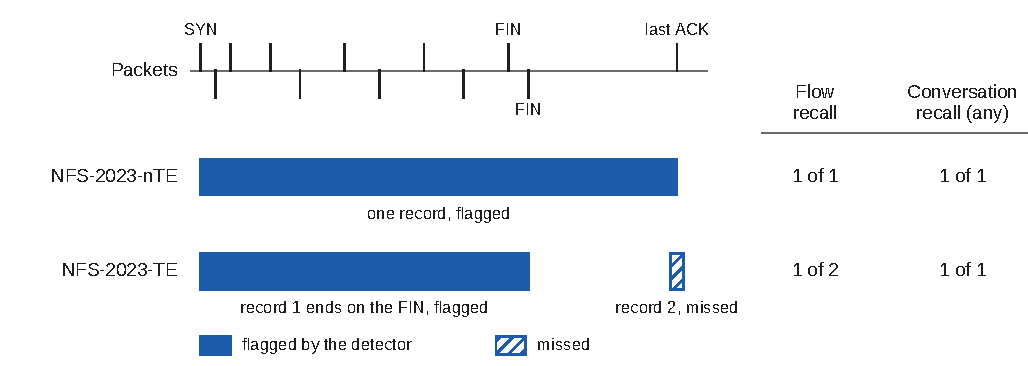
\includegraphics[width=\textwidth]{fig_same_packets.pdf}
\caption{One TCP conversation as written by NFS-2023-nTE and NFS-2023-TE, two releases of the same capture that differ only in an expiry rule. Ticks above the line are packets from the initiator, ticks below are packets from the responder. The packet sequence is illustrative; the record boundaries follow the mechanism measured in Section~\ref{sec:rq3}, where the TE rule ends a record on the FIN and writes the last ACK of the close as a second record. A detector that flags the first record and misses the second halves flow-level recall on this conversation, while the conversation counts as detected under both rules}\label{fig:samepackets}
\end{figure*}

\begin{definition}[Exporter invariance]\label{def:invariance}
A metric $M$ is \emph{exporter invariant} on a benchmark when, for a fixed model family, a fixed training budget and a fixed split of the conversations, the expected value of $M$ is the same for every exporter up to sampling variation. A comparison of two releases by $M$ is \emph{defined} when $M$ is computed on the same population of conversations in both.
\end{definition}

Under this definition, flow-level metrics are not exporter invariant in general, by Eq.~\eqref{eq:flowrecall}. Whether conversation-level metrics are, once the population is fixed, is an empirical question: an exporter can still change what a detector learns, through its features and through how much of each conversation appears in training. RQ2 and RQ4 measure exactly that residual.

\subsection{Why the split also depends on the exporter}

The field's default protocol is a random stratified split of records. Under such a split, a conversation that an exporter writes as $n$ records sends each record to the test set with probability $q$, roughly independently. The probability that a conversation with at least one test record also has a record in training is
\begin{equation}\label{eq:leak}
\lambda(n) \;=\; \frac{1 - q^{n} - (1-q)^{n}}{1 - (1-q)^{n}},
\end{equation}
which is $0$ for $n = 1$ and, with $q = \SetTestFrac$, about $\SetLeakTwo$ for $n = 2$. So the amount of leakage a random split carries is itself a function of the exporter, through $n_j(c)$. A grouped split that assigns whole conversations to one side removes this term, provided the grouping key belongs to the traffic and not to one exporter's records. Eq.~\eqref{eq:leak} is our derivation; Section~\ref{sec:rq1} reports the leakage actually measured.

\subsection{Hypotheses}

Two hypotheses were fixed in writing before any model was trained (Section~\ref{sec:protocol}). H2: for small classes, the exporter explains more of the variance in per-class F1 than the model does, under the flow unit. H4: Kendall's $W$ of model rankings across exporters is higher at the conversation unit than at the flow unit.

%% =====================================================================
\section{Benchmarks and releases}\label{sec:data}
%% =====================================================================

We use only published flow releases; no packet capture was re-extracted by us. Table~\ref{tab:arms} lists the ten arms. For \cicids{} we use the release of the original authors (the GeneratedLabelledFlows files, which carry the five-tuple and a timestamp; the better known machine learning CSV files have the same row count, \NcicRows{}, but neither), WTMC-2021 \cite{engelen2021}, CRiSIS-2022 \cite{lanvin2023}, LYCOS-IDS2017 \cite{rosay2021}, NFS-2023-nTE and NFS-2023-TE \cite{pekar2024}, and BCCC-CIC-IDS2017 \cite{shafi2024}. For UNSW-NB15 we use the four original CSV files \cite{moustafa2015}, NF-UNSW-NB15-v3 \cite{luay2026} and CIC-UNSW-NB15 \cite{mohammadian2024}, of which we use the file of all labelled flows rather than the subsample its authors distribute for training. Two further releases could not be used: HERA versions of \cicids{} \cite{pinto2025} have been requested from the authors, and Xin et al.\ released code but no flow tables \cite{xin2026}.

% Generated by 03_Code/make_numbers.py from 04_Results/release_inventory.csv, phase4/arm_durations.csv. Do not edit by hand.
\begin{table*}[t]
\caption{The ten arms. Records: rows in the release as used (UNSW-NB15 original after dropping
three lines repeated at file boundaries). Longest record: the longest record duration observed in
the arm, which reveals an active timeout where one is applied. Clock: time base and resolution of
the start time as found when reconciling clocks (Section~\ref{sec:clocks}).}\label{tab:arms}
\small
\begin{tabularx}{\textwidth}{@{}>{\raggedright\arraybackslash}p{2.5cm}>{\raggedright\arraybackslash}p{3.0cm}r>{\raggedright\arraybackslash}p{1.5cm}L@{}}
\toprule
Arm & Exporter & Records & Longest record & Clock \\
\midrule
\multicolumn{5}{@{}l}{\cicids{}} \\
CIC original & CICFlowMeter & 2{,}830{,}743 & 120 s & Local ADT, 12 hour clock without AM or PM; minutes (Monday: seconds) \\
WTMC-2021 & CICFlowMeter, corrected & 2{,}100{,}814 & 120 s & CEST, seconds \\
CRiSIS-2022 & CICFlowMeter, corrected & 2{,}104{,}683 & 120 s & Local ADT, 24 hour clock, seconds \\
LYCOS & LycoSTand & 1{,}837{,}498 & 120 s & UTC epoch, microseconds \\
NFS-2023-nTE & NFStream, no flag expiry & 2{,}111{,}131 & 120 s & UTC epoch, milliseconds \\
NFS-2023-TE & NFStream, FIN and RST expiry & 3{,}153{,}360 & 120 s & UTC epoch, milliseconds \\
BCCC & NTLFlowLyzer & 2{,}438{,}052 & 30{,}155 s & UTC minus 4, microseconds \\
\midrule
\multicolumn{5}{@{}l}{UNSW-NB15} \\
Original & Argus and Bro-IDS & 2{,}540{,}044 & 8{,}787 s & UTC, seconds, rounded \\
NF-UNSW-NB15-v3 & nProbe (NetFlow v3) & 2{,}365{,}424 & about 121 s & UTC, milliseconds \\
CIC-UNSW-NB15 & CICFlowMeter & 3{,}540{,}241 & 120 s & UTC minus 4, 12 hour clock with AM or PM, seconds \\
\bottomrule
\end{tabularx}
\end{table*}

%% Records: cic_original, wtmc2021 and unsw totals from 04_Results/count_check.csv;
%% NFS totals are the sums of the per day counts in count_check.csv (Pekar and Jozsa Table 2).
%% CRiSIS, LYCOS and BCCC totals: sums of rows in 04_Results/release_inventory.csv (LYCOS ships without Thursday afternoon).
%% Longest record: 04_Results/phase4/arm_durations.csv. Clocks: 04_Results/release_clock_summary.csv.

Every release was checked against the counts its authors publish before use. \NcountChecksMatched{} \NcountChecks{} checks matched exactly, including the per-day flow and attack counts of five releases in Table~\litnum{2} of Pekar and Jozsa \cite{pekar2024} the totals stated on the UNSW-NB15 and NetFlow v3 pages, and the per-class counts on the CIC-UNSW-NB15 page. The one mismatch on a first pass, three lines too many in UNSW-NB15, comes from the second, third and fourth CSV files each repeating the last line of the previous file; the loader drops them. Three properties of the releases matter for what follows. The original \cicids{} start times have minute resolution, so nothing finer than a minute can be compared against that arm. The LYCOS release ships without labels and was labelled with the authors' own script, unchanged. BCCC ships one file per class rather than per day and has no infiltration file.

%% =====================================================================
\section{Method}\label{sec:method}
%% =====================================================================

The instrument has five parts: one clock, one conversation key, one ground truth, one alignment and one pair of splits. Everything downstream reads a single frozen table per benchmark and day, written with a manifest of input hashes, settings and the code version. Two runs of the whole pipeline from fresh clones of the repository wrote identical frozen tables; their predictions and result files differ only in recorded run times and in the values that a code fix between the two runs changed. Fig.~\ref{fig:instrument} shows the parts and the analyses that read the frozen table.

\begin{figure*}[t]
\centering
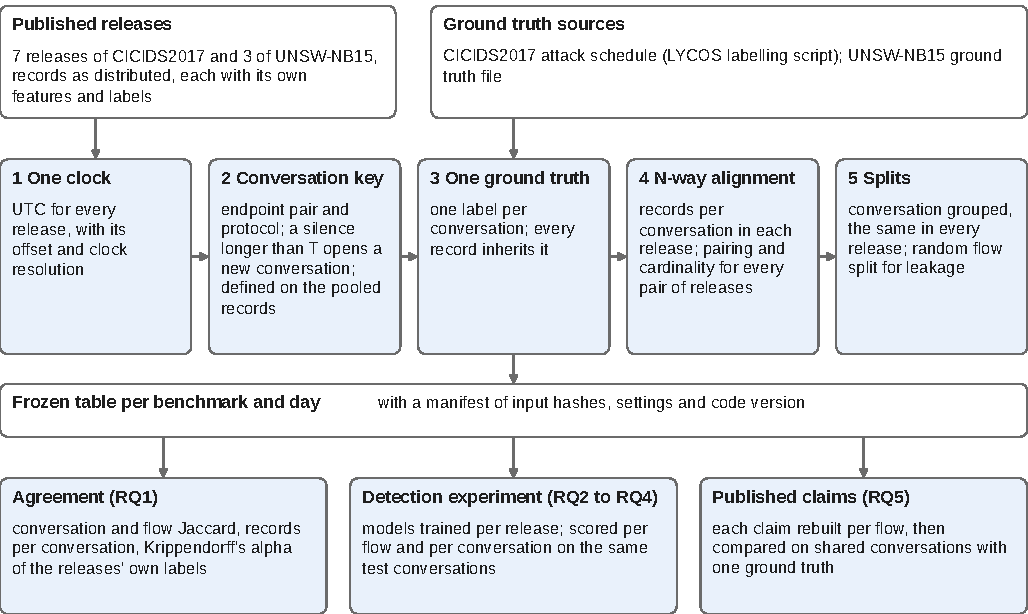
\includegraphics[width=\textwidth]{fig_instrument.pdf}
\caption{The instrument. Each release is read as distributed. The five parts, described in the subsections that follow, turn the releases of one benchmark into a frozen table per benchmark and day, and the three analyses read only that table. $T$ is the silence that ends a conversation (Section~\ref{sec:key})}\label{fig:instrument}
\end{figure*}

\subsection{One clock}\label{sec:clocks}

For each release we located the first and last record of known attacks and compared them with the published attack schedule. This fixed each release's time base (Table~\ref{tab:arms}). Two findings were not documented anywhere we looked. BCCC timestamps are one hour behind the capture's local time, UTC minus \NbcccOffset{}; with that offset, the first attack record in BCCC starts at the same microsecond as in LYCOS in \NbcccWindowsSame{} of the \NbcccWindows{} attack windows, and later in the other two. UNSW-NB15 start times are rounded to the nearest second rather than truncated: the NetFlow v3 start minus the original start is spread evenly over minus \setnum{0.5} to plus \setnum{0.5} seconds for \NunswOffsetShareA{} and \NunswOffsetShareB{} percent of paired flows on the two capture days. Read as truncated, \NunswTruncOutside{} percent of the paired flows on each day would fall outside their one-second window. CIC-UNSW-NB15 writes its start times as local time of the capture, UTC minus \docnum{4}, on a twelve-hour clock with AM or PM, to the second (Table~\ref{tab:arms}).

\subsection{Conversation key}\label{sec:key}

Records are blocked on the unordered pair of endpoints and the protocol, (address:port, address:port, protocol), with ports set to zero for protocols other than TCP and UDP. Only ICMP, TCP and UDP keep their protocol number and every other protocol forms one class, because Argus writes protocol names and \NprotoUnresolved{} percent of the rows of the UNSW-NB15 ground truth file name a protocol that the system table cannot resolve to a number, while nProbe writes numbers. Inside a block, records are ordered by start time, and a record that begins more than $T$ seconds after every earlier record of the block has ended opens a new conversation. Each record covers its start time plus its duration plus the resolution of its release's clock, so that coarse clocks cannot create false gaps. The initiator is the source endpoint of the earliest record.

The key is pooled: conversations are defined on the records of all arms together, so that they belong to the traffic and not to one exporter. A per-arm definition would let the test populations differ between arms, which is the confound under study. The CIC original arm does not take part in defining conversations, for one reason: its start times have minute resolution, so each of its records covers its duration plus up to a minute. Pooled with the others, such a record would bridge any silence shorter than a minute between two uses of an endpoint pair, which the six clocks with second or finer resolution can see, and the conversation set of the whole benchmark would then be set by the coarsest clock. Its records are mapped afterwards onto the conversation they can reach. At most \NnondefUnmappedMax{} of its records per day reach none, and between \NnondefAmbigMin{} and \NnondefAmbigMax{} per day reach more than one candidate, out of \NcicDayRecordsMin{} to \NcicDayRecordsMax{} records per day.

Because the key is pooled, the conversation set depends on which releases define it. Adding CIC-UNSW-NB15 as a defining arm changed the UNSW-NB15 conversations, and a different set of releases would give a somewhat different set of conversations. Definition~\ref{def:invariance} is therefore relative to the arm set that defines $C$. We measured how much this matters by rebuilding the conversations with each defining arm left out in turn and, for \cicids{}, with CIC original added as a defining arm, and comparing each rebuilt set with the frozen one on the records both contain. Leaving out any defining arm other than BCCC-CIC-IDS2017 changes little: the Jaccard index between the rebuilt and the frozen conversation sets is at least \RevLooJaccOtherMinCic{} on \cicids{} and \RevLooJaccMinUnsw{} on UNSW-NB15, and at least \RevLooAttackMinUnsw{} for every UNSW-NB15 attack class. Leaving out BCCC-CIC-IDS2017 lowers it to \RevLooJaccMinCic{}. BCCC has no active timeout (Section~\ref{sec:rq1}), and without its long records some silences between two uses of an endpoint pair are no longer spanned, so the rebuilt set has more and shorter conversations. Benign traffic is affected most (\RevLooBenignDropBccc{}), and among attack classes the two slow denial-of-service tools, slowloris (\RevLooSlowlorisDropBccc{}) and slowhttptest (\RevLooSlowhttpDropBccc{}). Adding CIC original as a defining arm gives \RevLooJaccPlusOrig{} and, as its minute clock predicts, merges the conversations of the flooding attacks: the index is \RevLooHulkPlusOrig{} for DoS Hulk and \RevLooDdosPlusOrig{} for DDoS. The scores move much less than the conversation sets. Scoring the stored predictions on each rebuilt set without retraining, Kendall's $W$ of the model ranking at the conversation unit on \cicids{} ranges from \RevLooWMinCic{} to \RevLooWMaxCic{}, and no conversation F1 of any class in any arm changes by more than \RevLooFoneMaxChange{}. The conversations of the slow attacks on \cicids{}, and with them what Definition~\ref{def:invariance} compares, therefore depend on whether BCCC-CIC-IDS2017 is among the defining releases, and we report the defining set as part of the instrument.

We chose $T = \SetT$ s from a sweep over \SetSweep{} seconds on every day. On \cicids{} every scored class has the same number of conversations at every value from \NsweepCicStableMin{} to \NsweepCicStableMax{} seconds. Above that, two attack tools reuse endpoint keys: Friday DDoS falls from \NsweepDdosLow{} conversations at \NsweepCicStableMax{} seconds or less to \NsweepDdosSixty{} at \setnum{60} seconds and \NsweepDdosOneTwenty{} at \setnum{120} seconds, and Wednesday DoS Hulk falls from \NsweepHulkLow{} to \NsweepHulkOneTwenty{} at \setnum{120} seconds. On UNSW-NB15 no scored class changes by more than \NsweepUnswUpMax{} percent between \SetT{} and \NsweepCicStableMax{} seconds, but Generic is sensitive at the short end: at \NsweepCicStableMin{} seconds it has \NsweepGenericFivePct{} percent more conversations than at \SetT{} (\NsweepGenericFive{} against \NsweepGenericFifteen{} on one day). Benign counts move by at most \NsweepBenignMaxChange{} percent across the sweep. Fifteen seconds sits inside the stable range of \cicids{} and above the short end where UNSW-NB15 Generic splits, and is longer than every clock resolution except the minute clock, which does not define conversations. Section~\ref{sec:rq4} reruns the RQ4 conclusions at four other values of $T$.

\subsection{One ground truth}\label{sec:gt}

``Labels fixed'' means one label per conversation, from the attack schedule, the same in every arm; a record's label is the label of its conversation. For \cicids{} we reuse the schedule encoded in the LYCOS labelling script (attacker, victim, port, protocol and time window) unchanged, applied to the conversation's two endpoints in either order with the conversation start inside the window. We chose it over the NFS-2023 labeller because it can be read line by line and does not depend on the machine's time zone. The script's three drop rules (Thursday afternoon, which removes the infiltration class, and two sets of hosts on Friday) mark conversations as excluded: they stay in the tables but are neither split nor scored. This removes \NexclThursday{} conversations on Thursday and \NexclFriday{} on Friday. For UNSW-NB15 we use the ground truth file distributed with the dataset, matched on the same key; a conversation that meets several categories takes the most frequent. Each arm's own labels are kept beside the schedule label for the agreement analysis and as a sensitivity variant.

Labelling every record from its conversation is a choice with a cost. A record that an exporter writes after the attack payload has ended, such as the trailing record of RQ3, inherits the attack label although it carries no payload. The releases do not all see it that way: by their own labels, \NmixedTe{} percent of NFS-2023-TE attack conversations and \NmixedOrig{} percent of CIC original ones mix attack and benign records, against at most \NmixedOtherMax{} percent in the other releases. We keep the schedule label as the primary truth because it is the only one that is the same in every arm by construction, and we rerun the analyses that depend on such records under a payload-aware rule: a record keeps its conversation's schedule label when it carries payload and becomes benign when it carries none, PortScan excepted because a probe carries no payload by design. Payload is read from each release's own fields (payload byte counts for the CICFlowMeter releases and BCCC, non-empty packet counts for LYCOS); NFStream reports frame sizes rather than payload, so for the NFS-2023 releases a TCP record without payload is one whose largest frame is at most \setnum{74} bytes, an Ethernet, IPv4 and TCP header with the options of a SYN, and that has no packet with the PSH flag. On every attack class this rule turns the same number of conversations benign in the NFS-2023 releases as the payload byte counts do in WTMC-2021, within one conversation.

The ground truth decides what the comparison means, so we measured how each release's own labels agree with it. WTMC-2021, LYCOS and BCCC agree with the schedule on \NlabelGoodMin{} or more of the conversations of every class. CRiSIS-2022 and both NFS-2023 releases agree on \NlabelSlowhttp{} of slowhttptest and \NlabelSlowloris{} of slowloris conversations, and on \NlabelWebBf{} of web brute force and \NlabelXss{} of XSS conversations. WTMC-2021 marks most of exactly these conversations as attempted attacks, so the disagreement reflects a stated policy of those releases (an attack label only where attack payload is present), not a matching fault. Attempted attacks are kept under their schedule class in the primary analysis, because the attacker sent the traffic and an operator would want the attempt detected; folding them into benign and keeping them as a separate class are frozen as sensitivity settings.

\subsection{N-way alignment and the hand check}

For every conversation the frozen table records how many records each arm put in it, whether every arm has it, and for every pair of arms a cardinality class: one to one, one to many, many to one, many to many, or present in one arm only. Inside a conversation, records of two arms are paired by overlap of their time intervals under a one-to-one assignment, with unmatched records left explicit. We hand checked \NhandCases{} conversations, \NhandPerBench{} per benchmark, spanning every cardinality class, every arm pair on one \cicids{} day, and several attack classes. The check found four faults, three in the pairing rule and one in the key (protocol names against numbers). Each was fixed and turned into a unit test, and the \NhandCases{} cases are frozen as test fixtures.

\subsection{Agreement measures}\label{sec:agree}

For RQ1 we report, per benchmark, day, class and arm pair, the conversation Jaccard index (conversations both arms have, over conversations either has), the flow Jaccard index (paired records over the records of either arm, a paired record counted once), and the mean and distribution of flows per conversation. Label reliability is measured with Krippendorff's alpha for nominal data \cite{hayes2007}: the unit is a conversation present in at least two arms, the raters are the arms, and the value is the arm's own label for the conversation (an attack class if any of its records carries one, else benign). Our implementation agrees with an independent implementation to nine decimals on four random designs with missing values. Intervals are \setnum{95} percent percentile intervals from \SetBoot{} bootstrap resamples of conversations. We do not report alpha for the existence of conversations: the units are by construction conversations that at least one arm has, so joint absence cannot occur and alpha is pulled towards zero whatever the agreement. Existence is reported with the Jaccard index instead.

To explain splits, each record after the first in a conversation is classified by how it follows the previous one: a repeat (same start and duration), a tail (at most \SetTailMs{} ms long and starting within one second of the previous end), a cut (starting at least the arm's longest record duration minus one second after the previous start), an overlap, an idle split (starting more than one second after the previous end) or other. We compared these causes with the termination faults Engelen et al.\ document for CICFlowMeter \cite{engelen2021} and the five causes of Vormayr et al.\ \cite{vormayr2020}, and mark as not explained any class where they do not fit.

\subsection{Splits and leakage}

The conversation-grouped split sends each conversation to the test set when its seeded hash rank puts it in the lowest \SetTestPct{} percent of its class on that day, for seeds \SetSeeds{}. The same assignment is mapped into every arm, so every arm's test set holds the same traffic. The random flow split, the field's default, applies the same hash rank to each record, per arm and class. Leakage is the share of test conversations that have at least one record in training.

\subsection{Detection experiment}\label{sec:protocol}

The protocol, including the estimand, the factors, the analysis and the decision rules for H2 and H4, was committed to the project repository before any model was trained for it, in commit \docnum{\texttt{6f6756f}} of 27 October 2026, \docnum{08:50} (UTC\docnum{+6}). Two settings fixed afterwards from a time trial alone, the subsample and the size of the tuning grid, were written into the project log as dated addenda before the grid started and committed with the grid's results (commit \docnum{\texttt{2abace2}}). The protocols for RQ4 and RQ5 were committed before any of their numbers (commits \docnum{\texttt{dc20bb4}} and \docnum{\texttt{e0fe953}}); the RQ3 protocol was written into the project log before its first number and committed with its results (commit \docnum{\texttt{c3b0ef6}}), so for RQ3 the order rests on the log. A Git history records these times but does not certify them. The project repository that holds this history also holds private working notes and is not public; its full history is available to the editor and reviewers on request.

\paragraph{Factors.} Arm: the seven \cicids{} arms, and for UNSW-NB15 the original with exact duplicate lines dropped (primary, since the duplicates are a release artefact rather than exporter behaviour, Section~\ref{sec:rq1}), NF-UNSW-NB15-v3 and CIC-UNSW-NB15; the original as released and with near repeats collapsed are sensitivity arms outside the primary decomposition. Model: random forest, LightGBM and a small multilayer perceptron. Split: conversation grouped and random flow. Seed: \SetSeeds{}, selecting the split and the model's random state. Unit: flow and conversation, the latter under the ``any'' rule, with majority and byte-weighted rules kept for sensitivity. Population: each arm's own test records, and the common population of conversations present in every arm of the benchmark.

\paragraph{Fixed for every arm.} Each arm uses its own feature columns minus identifiers: addresses, ports, MAC and OUI fields, timestamps, flow identifiers, VLAN and tunnel identifiers, exporter bookkeeping fields, random protocol identifiers, and labels. Identifiers are removed because they let a model learn the testbed rather than the attack \cite{arp2022,flood2024}. The remaining categorical columns are coded by sorted level, infinite values become missing and missing becomes minus one; the multilayer perceptron sees a signed log transform followed by standard scaling fitted on training rows. Each model has one hyperparameter grid of \SetGridSize{} settings, the same for every arm, tuned on seed \setnum{0} of the grouped split by validation macro-F1 on \SetValPct{} percent of the training conversations; the chosen setting is then used for every split and seed of that arm. LightGBM uses an L2 penalty of \setnum{1} on leaf values in every fit, because without it training diverged on the first arm tuned. All days of a benchmark are pooled. To fit the grid on a laptop, conversations are subsampled by a hash independent of the split seeds: \SetBenignFraction{} of benign conversations, and at most \SetAttackCap{} conversations per attack class (this caps PortScan, DoS Hulk and DDoS in \cicids{} and Exploits in UNSW-NB15). The same conversations are kept in every arm, so the subsample changes class proportions identically for every exporter.

\paragraph{Responses and analysis.} Responses are per-class F1, macro-F1 over the classes with test support, macro-F1 over a fixed set of classes with at least \SetMinTest{} test conversations in every grouped seed, and the ranking of the models within each arm. The macro mean is also reported without Heartbleed, which has a single conversation. For each benchmark, split, unit, population and class, an ordinary least squares analysis of variance of per-class F1 on arm, model, their interaction and seed gives each factor's share of the total sum of squares. Kendall's $W$ \cite{kendall1939} measures agreement of model rankings with arms as raters. The population part of the exporter effect is the exporter share on the own population minus the exporter share on the common population. Intervals are \setnum{95} percent percentile intervals from a cluster bootstrap over conversations \cite{field2007} with \SetBoot{} resamples, drawn within schedule classes and the same for every cell so that arms and models stay paired. The conversation is the resampling unit because records of one conversation are not independent, which is the dependence RQ1 measures; seeds are not resampled, since each cell averages over its five seeds before the bootstrap statistic is formed.

\paragraph{Decision rules.} A class counts as small when it has fewer than \setnum{5{,}000} scored conversations; it is eligible for H2 when it has at least \SetMinTest{} test conversations in every grouped seed. The first threshold separates the classes whose test sets hold hundreds of conversations, where a few records more or less move F1, from the large classes capped by the subsample; with \SetMinTest{} test conversations, one conversation moves recall by at most \setnum{0.05}. Both were fixed in the protocol; the robustness analyses below vary them. In the primary setting (grouped split, flow unit, own population), a class is ``exporter above model'' when the interval of the exporter share minus the model share lies above zero. H2 holds in a benchmark when this is true for a strict majority of eligible small classes, and is judged supported overall if it holds in both benchmarks, not supported in neither, and mixed otherwise. H4 is judged on the bootstrap interval of the difference in $W$ between units (grouped split, common population).

\paragraph{Sanity check.} Three result cells drawn at random with a fixed seed from the finished table are recomputed by hand from the stored predictions.

\paragraph{Robustness analyses added after the primary results.} The following analyses were not in the protocol. They were added after the primary results were known, to test how far the verdicts depend on design choices, and they are reported beside the verdicts without replacing them. Variance shares per degree of freedom: each factor's sum of squares divided by its degrees of freedom, as a share of the sum of these over the factors, with H2 judged on them by the same interval rule. BCa intervals, with the acceleration estimated from a jackknife over \setnum{50} groups of conversations. H2 with each arm left out in turn, and over a grid of the two thresholds (small below \setnum{2{,}500}, \setnum{5{,}000} or \setnum{10{,}000} scored conversations; at least \setnum{10}, \setnum{20} or \setnum{40} test conversations). Precision and F1 reweighted to the class prevalence of the full data, each test conversation weighted by the inverse of its class's subsample fraction, in the bootstrap as well as the point estimate. The \cicids{} grid retrained on the payload-aware labels of Section~\ref{sec:gt}. The UNSW-NB15 grid retrained without the time-to-live fields (\texttt{sttl}, \texttt{dttl} and their equivalents in the other releases). The grouped-split grid extended with logistic regression and a $k$-nearest-neighbour classifier, each tuned once per arm like the other models. And a direct test of Definition~\ref{def:invariance} by two one-sided tests on between-arm F1 differences (Section~\ref{sec:rq4}).

%% Method subsections for RQ4 and RQ5 (Phase 7 and 8 protocols).
\subsection{Remedy and sensitivity}\label{sec:rq4method}

RQ4 reuses the grid of RQ2 and adds no new main model. H4 is judged on the common population with the schedule ground truth and the conversation-grouped split. Beside it we report, per class, the change in the exporter share from the flow unit to the conversation unit, with a paired bootstrap interval, and call it a fall or a rise when the interval excludes zero. A class has a large residual when its exporter share at the conversation unit is at least \setnum{0.25} and the arm means of its F1 spread by at least \setnum{0.05}. For each such class we break the errors down by arm: false negatives and false positives, whether a false positive's conversation has several records, and whether exactly one of them was flagged. Leave-one-arm-out shares, without intervals, show which arm carries a residual.

The sensitivity variants change one choice at a time: the gap $T$ (\setnum{5}, \setnum{30}, \setnum{60} and \setnum{120} seconds, with conversations rebuilt by the same code, which at \SetT{} seconds reproduces the frozen tables exactly), the aggregation rule (majority, byte-weighted), the unit (attack episodes in place of conversations), the treatment of attempted attacks (folded into benign) and the labels (each release's own in place of the schedule). The last two are run twice, once scoring the primary models against the changed labels and once retraining on them, the retraining on the grouped split and on \cicids{} only. For every variant we state which of five conclusions change: H4, H2 at the flow unit, H2 at the conversation unit, the per-class verdicts of exporter against model at the conversation unit, and the per-class direction of the exporter share.

\subsection{Re-examination of published claims}\label{sec:claims}

The claims for RQ5 were fixed in a table written before any RQ5 number was computed, so that they could not be chosen after seeing which survive. It lists \docnum{11} candidate claims from the papers of Section~\ref{sec:related}, of which five can be examined with released data (Table~\ref{tab:rq5}). The others need a re-extraction of the packet captures over a timeout grid \cite{janatiidrissi2025}, flows that have not been released \cite{pinto2025,xin2026}, or benchmarks outside our scope \cite{vitorino2025}. For BCCC-CIC-IDS2017 we have not read the claim text, and NF-UNSW-NB15-v3 makes no performance comparison \cite{luay2026}.

Each examinable contrast goes through three steps. First, the comparison is rebuilt per flow the way the authors made it, on their releases with their own labels, preprocessing, features and model, using the authors' code where it is public and a line-by-line port of it where needed, refitted with seeds \SetSeeds{}. We do not claim to reproduce their exact experiment, and we state where our setup departs from theirs. Second, the per-flow gap $G$ is split into a part from classes that only one release has and, on the shared classes, a class weight part $C$ and a within-class part $W$. $C$ is the symmetric two-fold reweighting of the test records of each release to the class shares of the other, in the manner of an Oaxaca decomposition, and $W = G_{\mathrm{shared}} - C$. Third, the same contrast is computed on the conversations of the subsample of Section~\ref{sec:protocol} that have records in both releases, with the schedule ground truth, the conversation-grouped split, the claim's own model and features, and the ``any'' rule. Intervals are paired cluster bootstrap intervals over conversations with \SetBoot{} resamples. The verdict is read from the conversation-level gap in the claim's own metric. A claim survives when the gap has the published sign and its interval excludes zero, reverses when the interval lies entirely on the other side, and is not supported otherwise. A claim of no difference survives when the interval lies within \setnum{0.01} of zero and is contradicted when it excludes zero. A class with fewer than \SetMinTest{} test conversations in any seed is not estimable.


\subsection{Reproducibility}

Every number in this paper is produced by a script from the released data, and the text and tables take every number from one generated file of macros, so no number is typed by hand. Each script writes a manifest with SHA-256 hashes of its inputs and outputs, its parameters, the code version and the package versions. Two complete runs of the pipeline from fresh clones of the repository read byte-identical inputs (\docnum{502} files, hashed). Between the two runs, every stored prediction file was byte identical except \docnum{ten} that a code fix changed, the result tables differed only in recorded run times and in the values changed by the two fixes made between the runs, \docnum{286} of \docnum{287} number macros and \docnum{seven} of \docnum{eight} figure files were byte identical, and the values reported are those of the second run. The third UNSW-NB15 release and the robustness analyses of Section~\ref{sec:protocol} were added afterwards and run once, with manifests, on the frozen results; they have not been through a second clean run. The code, the aggregate result tables and the manifests are public (\url{https://github.com/26sudipta/same-packets-different-scores}), and the version used for this paper is archived on Zenodo (\tocheck{DOI of the Zenodo deposit}). An AI assistant was used in this work; Section~\ref{sec:declarations} states how.

%% =====================================================================
\section{Results}\label{sec:results}
%% =====================================================================

\subsection{RQ1: releases agree on conversations, not on flows}\label{sec:rq1}

Table~\ref{tab:rq1-agreement} gives the answer at the level of whole benchmarks. On \cicids, flow counts differ between the seven releases by a factor of \RQoneFlowRatio{}, from \RQoneFlowsMin{} records (\RQoneFlowsMinArm{}) to \RQoneFlowsMax{} (\RQoneFlowsMaxArm{}) over the scored days, while conversation counts differ by \RQoneConvSpread{} percent. Over all \RQonePairs{} pairs of releases the conversation Jaccard index lies between \RQoneConvJaccardMin{} and \RQoneConvJaccardMax{}, and the flow Jaccard index between \RQoneFlowJaccardMin{} and \RQoneFlowJaccardMax{}. The releases see the same connections. They disagree on how to cut them.

% Generated by 03_Code/make_numbers.py from 04_Results/phase4. Do not edit by hand.
\begin{sidewaystable}
\caption{Conversations agree, flows do not. Ranges over the arms of each benchmark (seven for
\cicids, three for UNSW-NB15), all scored days pooled. Max/min is the largest count divided by the
smallest. Jaccard indices range over every pair of arms; for flows, two records count as the same
object when the instrument pairs them.}\label{tab:rq1-agreement}
\small
\setlength{\tabcolsep}{3pt}
\begin{tabular*}{\linewidth}{@{\extracolsep{\fill}}llrrrrrr@{}}
\toprule
 & & \multicolumn{2}{c}{Flows} & \multicolumn{2}{c}{Conversations} & \multicolumn{2}{c}{Jaccard over arm pairs} \\
\cmidrule(lr){3-4}\cmidrule(lr){5-6}\cmidrule(lr){7-8}
Benchmark & Class & Range & Max/min & Range & Max/min & Conversations & Flows \\
\midrule
\cicids & All scored & 1{,}837{,}498 to 2{,}826{,}174 & 1.54 & 1{,}715{,}520 to 1{,}718{,}583 & 1.00 & 0.997 to 1.000 & 0.649 to 0.999 \\
 & Benign & 1{,}395{,}666 to 2{,}051{,}926 & 1.47 & 1{,}279{,}344 to 1{,}282{,}070 & 1.00 & 0.996 to 1.000 & 0.671 to 0.998 \\
 & Attack & 441{,}623 to 774{,}248 & 1.75 & 435{,}630 to 436{,}513 & 1.00 & 0.998 to 1.000 & 0.570 to 0.999 \\
\midrule
UNSW-NB15 & All scored & 2{,}365{,}424 to 3{,}540{,}241 & 1.50 & 1{,}882{,}534 to 2{,}019{,}548 & 1.07 & 0.911 to 0.974 & 0.485 to 0.626 \\
 & Benign & 2{,}218{,}733 to 3{,}420{,}284 & 1.54 & 1{,}820{,}137 to 1{,}953{,}555 & 1.07 & 0.910 to 0.974 & 0.487 to 0.673 \\
 & Attack & 86{,}010 to 321{,}311 & 3.74 & 62{,}397 to 66{,}392 & 1.06 & 0.935 to 0.994 & 0.189 to 0.454 \\
\midrule
\begin{tabular}[t]{@{}l@{}}UNSW-NB15,\\duplicates dropped\end{tabular} & All scored & 2{,}059{,}414 to 3{,}540{,}241 & 1.72 & 1{,}882{,}534 to 2{,}019{,}548 & 1.07 & 0.911 to 0.974 & 0.485 to 0.733 \\
 & Benign & 1{,}959{,}743 to 3{,}420{,}284 & 1.75 & 1{,}820{,}137 to 1{,}953{,}555 & 1.07 & 0.910 to 0.974 & 0.487 to 0.734 \\
 & Attack & 86{,}010 to 119{,}957 & 1.39 & 62{,}397 to 66{,}392 & 1.06 & 0.935 to 0.994 & 0.438 to 0.709 \\
\bottomrule
\end{tabular*}
\end{sidewaystable}


\paragraph{The disagreement depends on the class.} Table~\ref{tab:rq1-fpc} and Fig.~\ref{fig:fpc} restrict the comparison to conversations present in every arm, so that each column describes the same traffic. PortScan stays at \RQonePortscanFpc{} flows per conversation in every release: a probe of one or two packets has nothing to split. FTP-Patator is written as one record per conversation by \RQoneFtpOneArms{} releases and as \RQoneFtpSplitRange{} records by the other \RQoneFtpSplitArms{} (CIC original, NFS-2023-TE and BCCC). SSH-Patator, the three web attacks and Bot follow the same split between the same releases. DoS Hulk separates the releases differently again: one record per conversation in \RQoneHulkOneArms{} of them, \RQoneHulkOrig{} in CIC original, \RQoneHulkBccc{} in BCCC and \RQoneHulkTe{} in NFS-2023-TE. Averaged over attack classes the way a macro-F1 averages, the same attack traffic carries \RQoneMacroBccc{} flows per conversation in BCCC, \RQoneMacroCorrected{} in WTMC-2021, CRiSIS-2022 and LYCOS, and \RQoneMacroTe{} in NFS-2023-TE. These macro means include Heartbleed, a single connection written as \RQoneHeartbleedRecords{} records by every release except BCCC, which writes one.

% Generated by 03_Code/make_numbers.py from 04_Results/phase4. Do not edit by hand.
\begin{table}[t]
\caption{Mean flows per conversation, \cicids, all days pooled, on the conversations present in
every arm, so each column describes the same traffic. Conv.: how many such conversations the class
has. The macro mean is the unweighted mean over attack classes, the average a macro-F1
inherits; the last row leaves out Heartbleed, a single conversation, as the macro-F1 of the
detection experiment does (Section~\ref{sec:protocol}).}\label{tab:rq1-fpc}
\small
\setlength{\tabcolsep}{3pt}
\begin{tabular}{lrrrrrrrr}
\toprule
Class & Conv. & \rotatebox{90}{CIC original} & \rotatebox{90}{WTMC-2021} & \rotatebox{90}{CRiSIS-2022} & \rotatebox{90}{LYCOS} & \rotatebox{90}{NFS-2023-nTE} & \rotatebox{90}{NFS-2023-TE} & \rotatebox{90}{BCCC} \\
\midrule
Benign & 1{,}276{,}869 & 1.50 & 1.10 & 1.10 & 1.09 & 1.11 & 1.60 & 1.40 \\
Bot & 736 & 2.00 & 1.00 & 1.00 & 1.00 & 1.00 & 2.00 & 1.96 \\
DDoS & 93{,}122 & 1.71 & 1.03 & 1.03 & 1.03 & 1.00 & 2.06 & 1.03 \\
DoS GoldenEye & 6{,}692 & 1.44 & 1.01 & 1.03 & 1.01 & 1.06 & 2.05 & 1.00 \\
DoS Hulk & 157{,}952 & 1.50 & 1.00 & 1.00 & 1.00 & 1.00 & 2.37 & 2.21 \\
DoS Slowhttptest & 4{,}369 & 1.37 & 1.14 & 1.14 & 1.11 & 1.37 & 1.52 & 1.17 \\
DoS Slowloris & 3{,}869 & 1.59 & 1.47 & 1.47 & 1.46 & 1.80 & 1.90 & 1.13 \\
FTP-Patator & 3{,}992 & 2.37 & 1.00 & 1.00 & 1.00 & 1.00 & 2.00 & 2.39 \\
Heartbleed & 1 & 12.00 & 11.00 & 11.00 & 11.00 & 11.00 & 12.00 & 1.00 \\
PortScan & 159{,}687 & 1.00 & 1.00 & 1.00 & 1.00 & 1.00 & 1.00 & 1.01 \\
SSH-Patator & 2{,}959 & 2.00 & 1.00 & 1.00 & 1.00 & 1.00 & 2.01 & 2.00 \\
Web brute force & 1{,}361 & 2.00 & 1.00 & 1.00 & 1.00 & 1.00 & 2.02 & 2.00 \\
Web SQL injection & 12 & 2.00 & 1.00 & 1.00 & 1.00 & 1.00 & 2.00 & 2.00 \\
Web XSS & 662 & 2.00 & 1.00 & 1.00 & 1.00 & 1.00 & 2.05 & 2.00 \\
\midrule
Macro mean, attacks &  & 2.54 & 1.82 & 1.82 & 1.82 & 1.86 & 2.69 & 1.61 \\
Macro mean, without Heartbleed &  & 1.75 & 1.06 & 1.06 & 1.05 & 1.10 & 1.91 & 1.66 \\
\bottomrule
\end{tabular}
\end{table}


\begin{figure*}[t]
\centering
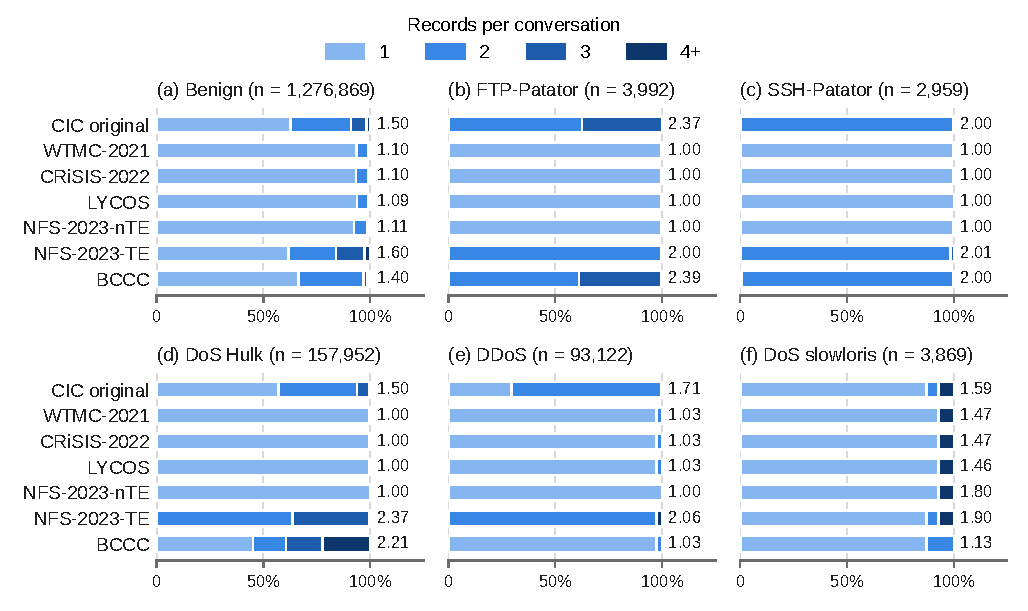
\includegraphics[width=\textwidth]{fig1_flows_per_conversation.pdf}
\caption{Records per conversation for six \cicids{} classes, on conversations present in every arm. Each bar shows the share of conversations written as one, two, three, or four or more records; the number at the bar end is the mean. The classes were chosen to show three behaviours (tail records doubling a class, releases disagreeing with each other on one class, and timeout cuts); Table~\ref{tab:rq1-fpc} gives the mean for every class}\label{fig:fpc}
\end{figure*}

\paragraph{Mechanisms.} Most of the pattern traces to named termination rules. The three releases that double FTP-Patator, SSH-Patator, the web attacks and Bot write an extra record at the end of a TCP connection. In NFS-2023-TE, \RQoneTailFtpTe{} percent of the extra FTP-Patator records are tails of at most \SetTailMs{} ms that start within a second of the previous record's end, and in BCCC \RQoneTailBccc{} percent of the extra records in these classes are tails. This matches the flow termination fault Engelen et al.\ describe for CICFlowMeter, where a flow ends at the first FIN packet, so the packets that follow it open a new flow \cite{engelen2021}, and the FIN and RST based expiry that distinguishes NFS-2023-TE from nTE \cite{pekar2024}. Long, sparse connections are cut by the \NactiveTimeout{} second active timeout: \RQoneCutSlowloris{} percent of the extra slowloris records in WTMC-2021, CRiSIS-2022 and LYCOS are such cuts, and the single Heartbleed connection becomes \RQoneHeartbleedCut{} records. BCCC shows no active timeout at all (its longest record lasts \RQoneBcccLongest{} seconds), which is why it writes Heartbleed as one record and splits slowloris least. Every attack class except PortScan therefore changes its weight in a flow-level average according to which of two independent rules, connection teardown and active timeout, a release applies.

Three further behaviours we traced to the exporters' termination code, reading NFStream at version \docnum{6.5.4} and NTLFlowLyzer as released, and to the flag and payload fields of the records. Both NFS-2023 releases split slowloris and slowhttptest more often than the \NactiveTimeout{} second timeout predicts: \RQoneIdleNfs{} percent of their extra records in these two classes are idle splits, which start more than one second after the previous record ends. All \RevIdleNte{} idle splits in NFS-2023-nTE, and \RevIdleTeSixty{} of \RevIdleTe{} in NFS-2023-TE, follow a silence of at least \setnum{60} seconds (median \RevIdleGapLoris{} seconds for slowloris and \RevIdleGapHttp{} for slowhttptest). NFStream expires a flow when the time since its last packet reaches the idle timeout, which these releases set to \setnum{60} seconds \cite{pekar2024}, and the slow attacks leave longer pauses than that; releases without a \setnum{60} second idle timeout do not split at these pauses. The split records still fall in one conversation although the pause exceeds $T$, because records of the other releases span it. BCCC splits DoS Hulk (\RQoneHulkBccc{}) but hardly DDoS (\RQoneDdosBccc{}) or GoldenEye (\RQoneGoldenBccc{}), although all three are HTTP floods. NTLFlowLyzer ends a flow when the next packet of its five-tuple arrives after the flow has seen a RST, or a FIN in each direction, and that packet opens a new flow. Of the \RevHulkExtra{} extra DoS Hulk records in BCCC, \RevHulkAfterRst{} follow a record that already had a RST and \RevHulkAfterFin{} one with a FIN in each direction; \RevHulkCarryRst{} carry a RST themselves and \RevHulkNoPay{} carry no payload. They are packets that arrive after the connection was torn down. All \RevGoldenConvs{} GoldenEye conversations in BCCC are single records, and the \RevDdosExtra{} extra DDoS records among \RevDdosConvs{} conversations all follow a RST, so the rule is the same for the three floods and the difference lies in how often packets follow the teardown. The third FTP-Patator record, present in \RQoneFtpThreeOrig{} percent of conversations in CIC original and \RQoneFtpThreeBccc{} percent in BCCC but not in NFS-2023-TE, has the same cause in BCCC: \RevFtpBcccExtraRst{} of its \RevFtpBcccExtra{} extra records carry a RST. In CIC original it is only partly explained. Of \RevFtpOrigExtra{} extra records, \RevFtpOrigSyn{} carry a SYN and \RevFtpOrigNoPay{} no payload, and the median extra record has \RevFtpOrigPk{} packets, so most are neither new connections nor empty tails. That fits a flow ended at the first FIN while the session goes on, the fault Engelen et al.\ describe \cite{engelen2021}, but we have not confirmed it in the code of the CICFlowMeter version that produced the release.

\paragraph{Pairwise structure.} The disagreement is not a small perturbation. Against WTMC-2021, the CIC original release agrees one to one on \RQoneOrigWtmcOneOne{} of conversations and is many to one on \RQoneOrigWtmcManyOne{}.

\paragraph{Leakage under the field's default split.} Because the releases cut conversations differently, the random flow split leaks different amounts of traffic in each. Pooled over days, classes and seeds, the share of test conversations with a record in training is \RQoneLeakOrig{} for CIC original, \RQoneLeakTe{} for NFS-2023-TE and \RQoneLeakBccc{} for BCCC, the three releases that write tail records, against \RQoneLeakLow{} for WTMC-2021, CRiSIS-2022, LYCOS and NFS-2023-nTE. On UNSW-NB15 it is \RQoneLeakUnswOrig{} for the original, \RQoneLeakUnswVthree{} for NF-UNSW-NB15-v3 and \RQoneLeakUnswCic{} for CIC-UNSW-NB15, the largest of any release. Under the conversation-grouped split it is zero for every arm, day, class and seed, by construction. The ordering follows Eq.~\eqref{eq:leak}: releases with more records per conversation leak more (Fig.~\ref{fig:leak}). A score obtained under a random flow split on one release has thus been measured with a different amount of leakage than the same model's score on another release.

\begin{figure}[t]
\centering
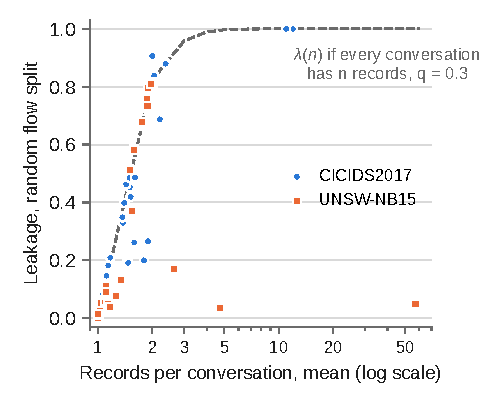
\includegraphics{fig2_leakage.pdf}
\caption{Leakage of the random flow split against the mean number of records per conversation, one point per release and class (scored days and five seeds pooled; releases as published, so UNSW-NB15 keeps its duplicate lines). The dashed line is $\lambda(n)$ of Eq.~\eqref{eq:leak} with $q = \SetTestFrac$, the leakage of a class whose every conversation has exactly $n$ records. Points below it belong to classes in which most conversations have a single record and a few have many, so the mean overstates the typical count}\label{fig:leak}
\end{figure}

\paragraph{Label agreement.} Table~\ref{tab:rq1-alpha} reports how far the releases' own labels agree on shared conversations. On \cicids{} Krippendorff's alpha is \RQoneAlphaCic{} (interval \RQoneAlphaCicLo{} to \RQoneAlphaCicHi{}) over \RQoneAlphaCicUnits{} conversations, with observed agreement \RQoneAlphaCicObs{}. By day it is \RQoneAlphaTuesday{} on Tuesday, \RQoneAlphaWednesday{} on Wednesday and \RQoneAlphaFriday{} on Friday, but \RQoneAlphaThursday{} on Thursday, the day on which three releases label web attacks as benign under their payload rule (Section~\ref{sec:gt}). Pairs of releases show where the Thursday value comes from. CIC original, WTMC-2021, LYCOS and BCCC agree with each other (pairwise alpha at least \RQoneThuWithinMin{}), CRiSIS-2022 and NFS-2023-nTE agree with each other (\RQoneThuGroupTwo{}), and every pair across the two groups has alpha between \RQoneThuCrossMin{} and \RQoneThuCrossMax{}. The second group applies the payload rule. When the attempted attacks that WTMC-2021 marks are read as benign, WTMC-2021 agrees with both releases of the second group (alpha \RQoneThuWtmcAttBenign{}), so the payload policy accounts for the split into two groups. NFS-2023-TE agrees with no other release on Thursday (alpha \RQoneThuTeMin{} to \RQoneThuTeMax{}); we have not traced the cause of this further disagreement. Monday has no attacks, so alpha is undefined there. On UNSW-NB15 alpha is \RQoneAlphaUnsw{} (\RQoneAlphaUnswLo{} to \RQoneAlphaUnswHi{}) over \RQoneAlphaUnswUnits{} conversations, with observed agreement \RQoneAlphaUnswObs{}. NF-UNSW-NB15-v3 marks \RQoneVthreeExtraA{} records on one day and \RQoneVthreeExtraB{} on the other as attacks in conversations that the ground truth file leaves benign, which likely explains most of the gap; how that release assigned its labels has not been checked. The intervals resample conversations as if independent, so they are too narrow if anything, since conversations of one attack episode are not independent. These values matter for the next questions in a specific way: they show that the releases' own labels are not interchangeable on some days, which is why the detection experiment uses one schedule ground truth.

% Generated by 03_Code/make_numbers.py from 04_Results/phase4. Do not edit by hand.
\begin{table}[t]
\caption{Agreement of the arms' own labels, Krippendorff's alpha (nominal). Unit: a conversation
present in at least two arms, all days pooled, excluded conversations left out. Raters: the arms,
each giving the conversation the label of its records (an attack class if any record carries one,
the most frequent such class). Interval: 95 percent, 1,000 bootstrap resamples of
conversations.}\label{tab:rq1-alpha}
\small
\setlength{\tabcolsep}{3pt}
\begin{tabular}{llrrrr}
\toprule
Benchmark & Labels & Units & Obs. & $\alpha$ & 95\% interval \\
\midrule
\cicids & Class & 1{,}718{,}246 & 0.995 & 0.988 & 0.988 to 0.988 \\
 & Attack or benign & 1{,}718{,}246 & 0.995 & 0.987 & 0.986 to 0.987 \\
 & Attempted as benign & 1{,}718{,}246 & 0.995 & 0.988 & 0.988 to 0.988 \\
UNSW-NB15 & Class & 2{,}016{,}038 & 0.986 & 0.824 & 0.822 to 0.826 \\
 & Attack or benign & 2{,}016{,}038 & 0.986 & 0.823 & 0.821 to 0.824 \\
\begin{tabular}[t]{@{}l@{}}UNSW-NB15,\\duplicates dropped\end{tabular} & Class & 2{,}016{,}038 & 0.986 & 0.824 & 0.822 to 0.825 \\
 & Attack or benign & 2{,}016{,}038 & 0.986 & 0.823 & 0.821 to 0.824 \\
\bottomrule
\end{tabular}
\end{table}


\paragraph{Duplicate lines in UNSW-NB15.} On UNSW-NB15, the original release has \RQoneUnswAttackRatio{} times as many attack flows as NF-UNSW-NB15-v3 (\RQoneUnswAttackOrig{} against \RQoneUnswAttackVthree{}), while attack conversations differ by a factor of \RQoneUnswAttackConvRatio{} over the three releases. Most of that gap is not an exporter effect. The original CSV files hold \RQoneUnswDups{} surplus lines that are identical to another line in all \docnum{49} fields (\RQoneUnswDupsA{} on the first capture day and \RQoneUnswDupsB{} on the second), counted by hashing raw lines and equal to the count from sorting the raw files minus the three boundary repeats. With them dropped, the attack flow ratio falls to \RQoneUnswAttackRatioDedup{} and the attack flow Jaccard index rises from \RQoneUnswAttackJaccard{} to \RQoneUnswAttackJaccardDedup{}. After exact duplicates are removed, a further \RQoneNearB{} records on the second day (\RQoneNearA{} on the first) repeat the five-tuple, start, end and byte count of an earlier record; of the first \RQoneNearSample{} of them on the second day, \RQoneNearAttackCat{} differ from that earlier record only in the attack category and \RQoneNearCt{} only in the windowed count features. We treat exact duplicates as a release artefact and drop them for RQ1 and RQ2, keep the release as published for RQ5, where published results used it, and collapse the near repeats in a sensitivity run. Duplication in UNSW-NB15 has been reported before for the training and testing partition that the dataset's authors distribute beside the full files: Al-Daweri et al.\ found duplicated records in its training set and none in its testing set \cite{aldaweri2020}. In a targeted search we found no earlier count for the four full CSV files used here.

\paragraph{CIC-UNSW-NB15 cuts the attacks finer.} The third UNSW-NB15 release agrees with the others on which attack conversations occurred (conversation Jaccard index \RQoneUnswAttackConvJaccardOrigCicDedup{} against the deduplicated original and \RQoneUnswAttackConvJaccardVthreeCic{} against NF-UNSW-NB15-v3) and cuts them into more records: \RQoneCicUnswAttackFpc{} records per attack conversation, and \RQoneUnswAttackOneNOrigCicDedup{} percent of the attack conversations it shares with the deduplicated original are one record there and several in CIC-UNSW-NB15. The attack flow Jaccard index is \RQoneUnswAttackJaccardOrigCicDedup{} against the deduplicated original and \RQoneUnswAttackJaccardVthreeCic{} against NF-UNSW-NB15-v3. CIC-UNSW-NB15 is produced by CICFlowMeter, the extractor whose termination fault Engelen et al.\ describe \cite{engelen2021}; we did not trace which of its rules splits the UNSW-NB15 attacks.

\paragraph{Answer to RQ1.} Releases of the same benchmark agree almost perfectly on which conversations occurred and disagree widely, and by class, on how many flows each conversation becomes. The disagreement follows two termination rules that releases apply independently, it changes the leakage of the field's default split by a factor of more than \RQoneLeakFactor{} between releases, and on UNSW-NB15 most of the apparent difference between the original and its NetFlow version is duplicated lines rather than exporter behaviour, while CIC-UNSW-NB15 splits most attack conversations into several records.

\subsection{RQ2: population or detector}\label{sec:rq2}

The grid has \RQtwoCells{} cells: seven \cicids{} arms and five UNSW-NB15 arms (three primary, two for sensitivity), each crossed with three models, two splits and five seeds. Rerun from scratch, \RQtwoReproCells{} cells gave predictions identical row for row, and \RQtwoSanityCells{} cells drawn at random were recounted by hand from the stored predictions and match the results table. Unless stated otherwise, numbers below are from the primary setting: grouped split, flow unit, each arm's own population.

\paragraph{Scores move with the exporter.} On \cicids{} the mean macro-F1 over classes with test support ranges from \RQtwoMacroRfMin{} to \RQtwoMacroRfMax{} across arms for the random forest, from \RQtwoMacroLgbmMin{} to \RQtwoMacroLgbmMax{} for LightGBM and from \RQtwoMacroMlpMin{} to \RQtwoMacroMlpMax{} for the multilayer perceptron. NFS-2023-TE is the lowest arm for the random forest and LightGBM, and BCCC-CIC-IDS2017 is both the highest arm for the random forest and the lowest for the multilayer perceptron. On UNSW-NB15, NF-UNSW-NB15-v3 scores higher than the deduplicated original for every model (\RQtwoUnswVthreeMin{} to \RQtwoUnswVthreeMax{} against \RQtwoUnswDedupMin{} to \RQtwoUnswDedupMax{}), and CIC-UNSW-NB15 is the lowest arm for every model (\RQtwoUnswCicMin{} to \RQtwoUnswCicMax{}). Heartbleed has no test conversation in any grouped seed, so there the macro means with and without it coincide.

\paragraph{Exporter against model (H2).} Table~\ref{tab:rq2-shares} gives the variance shares for the small classes, the ones H2 is about. On \cicids{} the exporter explains more of the variance in per-class F1 than the model for \RQtwoExporterAboveCic{} of the \RQtwoEligibleCic{} eligible classes, and every one of the \RQtwoExporterAboveCic{} intervals excludes zero. The largest gaps are SSH-Patator (exporter share \RQtwoSshArm{}, model share \RQtwoSshModel{}) and Bot (\RQtwoBotArm{} against \RQtwoBotModel{}). Web XSS goes the other way (\RQtwoXssArm{} against \RQtwoXssModel{}). Web SQL injection, with \RQtwoSqliTest{} test conversations in its smallest seed, and Heartbleed, with none, are not eligible. On UNSW-NB15 the exporter leads for \RQtwoExporterAboveUnsw{} of \RQtwoEligibleUnsw{} eligible classes, every interval above zero; the narrowest lead is Worms (interval of the difference \RQtwoWormsLo{} to \RQtwoWormsHi{}). By the rule fixed in advance, H2 holds on both benchmarks. On UNSW-NB15 this verdict rests on CIC-UNSW-NB15. In a set of arms we added with that release, after the protocol was fixed, the original and NF-UNSW-NB15-v3 alone give \RQtwoUnswWithoutCicLeadN{} classes to the exporter (\RQtwoUnswWithoutCicLead{}), \RQtwoUnswWithoutCicModel{} to the model and leave \RQtwoUnswWithoutCicUndecided{} undecided, so without it H2 \RQtwoUnswWithoutCicHtwo{} on UNSW-NB15. Fig.~\ref{fig:h2} shows the contrast for every eligible class at both units.

The secondary settings agree with the primary one on \cicids{}. At the conversation unit the exporter leads for \RQtwoExporterAboveConvOwn{} of the \RQtwoEligibleCic{} eligible classes on the own population and \RQtwoExporterAboveConvCommon{} on the common one; DoS Slowhttptest turns to the model (difference \RQtwoSlowhttpConv{}, interval \RQtwoSlowhttpConvLo{} to \RQtwoSlowhttpConvHi{}). Under the random flow split the exporter leads for \RQtwoExporterAboveRandomOwn{} of \RQtwoEligibleCic{}, with DoS Slowhttptest undecided. On UNSW-NB15 neither sensitivity arm changes the verdict: by the same interval rule the exporter leads for \RQtwoUnswReleasedLeadN{} of \RQtwoEligibleUnsw{} classes with the original as published and for \RQtwoUnswCollapsedLeadN{} with its near repeats collapsed.

Two features of Table~\ref{tab:rq2-shares} matter for reading it. First, the interaction of exporter and model is large for several classes (\RQtwoInterWebBf{} for Web brute force, \RQtwoInterFtp{} for FTP-Patator, \RQtwoInterSlowloris{} for DoS Slowloris), so the size of the exporter effect depends on which model is trained. Second, the seed share is small: at most \RQtwoSeedCicMax{} on \cicids{} (\RQtwoSeedCicMaxClass{}), and \RQtwoSeedUnswGeneric{} for UNSW-NB15 Generic and \RQtwoSeedUnswBenign{} for its benign class. The split therefore moves per-class F1 far less than the exporter or the model does, on both benchmarks.

% Generated by 03_Code/make_numbers.py from 04_Results/phase5 (variance_shares, share_contrasts, h2_judgement). Do not edit by hand.
\begin{sidewaystable}
\caption{Share of the variance in per-class F1 explained by the exporter (arm), the model and their
interaction, for the small classes of the H2 test. Grouped split, flow unit, own population;
balanced analysis of variance over arm, model, arm by model and seed. Brackets are 95 percent
cluster bootstrap intervals over test conversations (1,000 resamples). Inter.: the arm by model
interaction. Test conv.: the smallest number of test conversations over the five grouped seeds.
The verdict uses the interval of the difference; \cicids{} has seven arms and UNSW-NB15 three (the
deduplicated original, NF-UNSW-NB15-v3 and CIC-UNSW-NB15).}\label{tab:rq2-shares}
\small
\begin{tabular*}{\linewidth}{@{\extracolsep{\fill}}lrlllll@{}}
\toprule
Class & Test conv. & Exporter & Model & Inter. & Exporter minus model & Verdict \\
\midrule
\multicolumn{7}{@{}l}{\emph{\cicids, seven arms}} \\
DoS Slowhttptest & 1{,}311 & 0.358 [0.316, 0.399] & 0.243 [0.208, 0.274] & 0.377 & 0.116 [0.049, 0.181] & Exporter \\
FTP-Patator & 1{,}198 & 0.489 [0.463, 0.515] & 0.079 [0.074, 0.083] & 0.431 & 0.411 [0.381, 0.440] & Exporter \\
DoS Slowloris & 1{,}160 & 0.407 [0.354, 0.460] & 0.151 [0.127, 0.171] & 0.421 & 0.256 [0.191, 0.325] & Exporter \\
SSH-Patator & 888 & 0.970 [0.966, 0.973] & 0.006 [0.005, 0.007] & 0.024 & 0.964 [0.960, 0.968] & Exporter \\
Web brute force & 408 & 0.314 [0.298, 0.326] & 0.033 [0.025, 0.042] & 0.609 & 0.280 [0.265, 0.292] & Exporter \\
Bot & 221 & 0.841 [0.829, 0.851] & 0.038 [0.034, 0.041] & 0.120 & 0.803 [0.788, 0.817] & Exporter \\
Web XSS & 199 & 0.214 [0.192, 0.233] & 0.639 [0.592, 0.663] & 0.135 & $-0.425$ [$-0.472$, $-0.358$] & Model \\
\midrule
\multicolumn{7}{@{}l}{\emph{UNSW-NB15, three arms}} \\
Generic & 1{,}049 & 0.943 [0.834, 0.953] & 0.029 [0.022, 0.060] & 0.019 & 0.914 [0.782, 0.931] & Exporter \\
DoS & 1{,}015 & 0.702 [0.663, 0.727] & 0.273 [0.242, 0.302] & 0.008 & 0.430 [0.361, 0.482] & Exporter \\
Shellcode & 420 & 0.878 [0.851, 0.896] & 0.098 [0.080, 0.118] & 0.017 & 0.780 [0.734, 0.816] & Exporter \\
Analysis & 113 & 0.694 [0.520, 0.743] & 0.109 [0.052, 0.183] & 0.060 & 0.585 [0.348, 0.682] & Exporter \\
Backdoor & 99 & 0.720 [0.606, 0.747] & 0.226 [0.166, 0.274] & 0.022 & 0.493 [0.347, 0.575] & Exporter \\
Worms & 43 & 0.552 [0.436, 0.608] & 0.312 [0.216, 0.378] & 0.078 & 0.240 [0.077, 0.381] & Exporter \\
\bottomrule
\end{tabular*}
\end{sidewaystable}


\paragraph{How far the H2 verdict depends on the design.} Table~\ref{tab:rev-robust} applies the H2 rule under settings that each remove one ground for doubt, with the same bootstrap resamples (Section~\ref{sec:protocol}). The arm factor has six degrees of freedom on \cicids{} and two on UNSW-NB15, against two for the model, so a raw share favours the arm. Compared per degree of freedom, the exporter still leads for \RevPerdfAboveCic{} of \RevEligCic{} eligible classes on \cicids{} and \RevPerdfAboveUnsw{} of \RevEligUnsw{} on UNSW-NB15, and H2 \RevPerdfHtwoCic{} on both. BCa intervals give the same verdict as the percentile intervals for all \RevBcaN{} eligible classes; for UNSW-NB15 Generic, whose percentile interval (\RevBcaGenericPctLo{} to \RevBcaGenericPctHi{}) sits against its estimate of \RevBcaGenericShare{}, the BCa interval is \RevBcaGenericLo{} to \RevBcaGenericHi{}. Over \RevThrSettings{} combinations of the two thresholds, which change the number of eligible classes from \RevThrEligMinCic{} to \RevThrEligMaxCic{} on \cicids{} and from \RevThrEligMinUnsw{} to \RevThrEligMaxUnsw{} on UNSW-NB15, H2 holds in every case. Leaving each arm out in turn, H2 holds in \RevSubHoldCic{} of \RevSubNCic{} arm sets on \cicids{}, never with fewer than \RevSubAboveMinCic{} classes to the exporter, and in \RevSubHoldUnsw{} of \RevSubNUnsw{} on UNSW-NB15, the exception being the set without CIC-UNSW-NB15 (\RevSubUnswNoCicAbove{} classes to the exporter, \RevSubUnswNoCicModel{} to the model). Reweighting the test set to the class prevalence of the full data keeps H2 on both benchmarks. Removing the TTL fields from every UNSW-NB15 arm, a check for a shortcut that these fields might offer, leaves the exporter ahead for \RevTtlAbove{} of \RevTtlElig{} classes, although the largest contrast, DoS, falls from \RevTtlDosWith{} to \RevTtlDosWithout{}. One setting does change the verdict. Under the payload-aware labels of Section~\ref{sec:rq3}, with every model retrained, the interval puts the exporter above the model for \RevPayAbove{} of \RevPayElig{} eligible \cicids{} classes and the model above the exporter for none; the point estimate favours the exporter for \RevPayPointAbove{}, but by the strict-majority rule H2 does not hold. Part of the exporter's lead on \cicids{} therefore comes from how records without payload are labelled, the same channel as in RQ3. With five models H2 holds on \cicids{} but not on UNSW-NB15 (Section~\ref{sec:rq4}).

% Generated by 03_Code/make_numbers.py from 04_Results/phase11/analysis. Do not edit by hand.
\begin{table}[t]
\caption{H2 under robustness settings, grouped split, flow unit, each arm's own population: eligible small classes for which the interval of the exporter share minus the model share lies above zero, out of the eligible classes. H2 holds when this is a strict majority. The rows on thresholds and on left-out arms count the settings in which H2 holds}\label{tab:rev-robust}
\small
\begin{tabular}{@{}lll@{}}
\toprule
Setting & \cicids{} & UNSW-NB15 \\
\midrule
Primary setting & 6 of 7 & 6 of 6 \\
Shares per degree of freedom & 4 of 7 & 6 of 6 \\
BCa intervals & 6 of 7 & 6 of 6 \\
Size and support thresholds varied & holds at 9 of 9 & holds at 9 of 9 \\
One arm left out, each in turn & holds in 7 of 7 & holds in 2 of 3 \\
Test set reweighted to full-data prevalence & 5 of 7 & 6 of 6 \\
Payload-aware labels (\cicids{} only) & 3 of 6 & n/a \\
TTL fields removed (UNSW-NB15 only) & n/a & 6 of 6 \\
Five models (adds logistic regression and $k$-NN) & 4 of 7 & 3 of 6 \\
\bottomrule
\end{tabular}
\end{table}


\begin{figure*}[t]
\centering
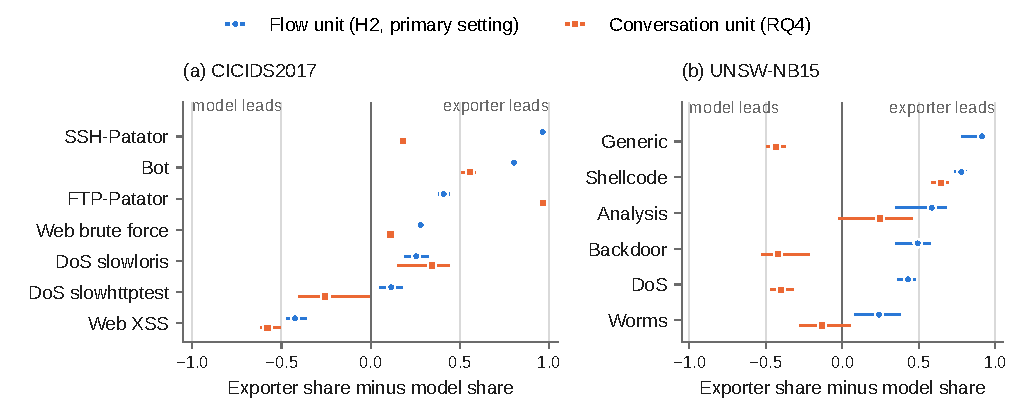
\includegraphics[width=\textwidth]{fig3_exporter_vs_model.pdf}
\caption{Exporter share minus model share of the variance in per-class F1, for the small classes eligible for H2 (grouped split, each arm's own population), with \setnum{95} percent cluster bootstrap intervals. Flow unit: the primary setting by which H2 is judged. Conversation unit: the same contrast when each conversation is scored once (RQ4). Right of zero, the exporter explains more of the variance than the model. Classes are ordered by the flow-unit contrast. (a) \cicids{}; (b) UNSW-NB15}\label{fig:h2}
\end{figure*}

\paragraph{Population part.} Scoring every exporter on the same conversations, the common population, barely changes the exporter share on \cicids{}. The own minus common difference is within \setnum{0.001} of zero for \RQtwoPopNearZero{} of the \RQtwoPopScored{} scored classes. Where it is clearly not zero it is negative, which means the exporter share \emph{grows} on the common population: PortScan \RQtwoPopPortscan{} (interval \RQtwoPopPortscanLo{} to \RQtwoPopPortscanHi{}) and DoS Slowloris \RQtwoPopSlowloris{} (\RQtwoPopSlowlorisLo{} to \RQtwoPopSlowlorisHi{}). DDoS (\RQtwoPopDdos{}) has an interval that includes zero. On UNSW-NB15 the difference is close to zero for Fuzzers \RQtwoPopUnswFuzzers{} (\RQtwoPopUnswFuzzersLo{} to \RQtwoPopUnswFuzzersHi{}), Reconnaissance \RQtwoPopUnswRecon{} (\RQtwoPopUnswReconLo{} to \RQtwoPopUnswReconHi{}) and Generic \RQtwoPopUnswGeneric{} (\RQtwoPopUnswGenericLo{} to \RQtwoPopUnswGenericHi{}); for the benign class it is positive, \RQtwoPopUnswBenign{} (\RQtwoPopUnswBenignLo{} to \RQtwoPopUnswBenignHi{}), so there part of the exporter share comes from scoring different conversations. With that exception, the exporter's effect on flow-level scores does not come from scoring different conversations. Restricting the test set to shared conversations fixes which conversations are scored but not how many records each one contributes, so the weights $w_j(c)$ of Eq.~\eqref{eq:flowrecall} still belong to the exporter. The comparison that fixes both, conversation unit on the common population, is the subject of RQ4.

\paragraph{Model rankings.} Kendall's $W$ of the model ranking across the seven \cicids{} arms is \RQtwoWFlow{} (interval \RQtwoWFlowLo{} to \RQtwoWFlowHi{}) at the flow unit and \RQtwoWConv{} (\RQtwoWConvLo{} to \RQtwoWConvHi{}) at the conversation unit, grouped split, each arm's own population; Table~\ref{tab:rq4-h4} gives the common population, on which H4 is judged. By mean macro-F1 the random forest or LightGBM ranks first and the multilayer perceptron last in \RQtwoMlpLastArms{} arm. On UNSW-NB15, with three primary arms, $W$ is \RQtwoWUnsw{} (\RQtwoWUnswLo{} to \RQtwoWUnswHi{}) at the flow unit, grouped split, and between \RQtwoWUnswMin{} and \RQtwoWUnswMax{} over every split, unit and population. H4 is judged in Section~\ref{sec:rq4}.

\paragraph{Where part of the exporter share comes from.} NFS-2023-TE scores between \RQtwoTeSmallMin{} and \RQtwoTeSmallMax{} F1 for SSH-Patator and Bot with every model. Without that arm, point estimates still put the exporter above the model for \RQtwoLoaoLead{} of the \RQtwoEligibleCic{} eligible \cicids{} classes, with smaller margins: the exporter share falls from \RQtwoSshArm{} to \RQtwoLoaoSshArm{} for SSH-Patator (model \RQtwoLoaoSshModel{}) and from \RQtwoBotArm{} to \RQtwoLoaoBotArm{} for Bot (model \RQtwoLoaoBotModel{}). With intervals, the verdict without NFS-2023-TE is the one in Table~\ref{tab:rev-robust}: H2 still holds. The cause of that arm's low scores is the subject of RQ3.

\subsection{RQ3: one expiry setting and the label policy}\label{sec:rq3}

NFS-2023-nTE and NFS-2023-TE were produced by the same tool from the same packets \cite{pekar2024}. TE turns on NFStream's rule that a TCP FIN or RST ends a flow, and a post-processing filter in that release then drops one-packet flows whose only packet is a FIN or RST. The contrast is therefore one generator setting plus the filter it triggers, not one setting alone. The two releases also come with different labels; scoring both against the schedule ground truth removes that difference, and scoring on the common population removes the difference in population. No model was trained for RQ3: the scores are the RQ2 grid cells of these two arms, averaged over three models and five seeds. The protocol and the direction of the prediction below were written before any RQ3 number was computed. Table~\ref{tab:rq3} covers the \RQthreeClasses{} attack classes with at least \SetMinTest{} common conversations in both arms; Heartbleed and Web SQL injection have fewer.

% Generated by 03_Code/make_numbers.py from 04_Results/phase6/table_6_1.csv. Do not edit by hand.
\begin{table*}[t]
\caption{NFS-2023-nTE against NFS-2023-TE on the common population. Records per conversation;
leakage, the share of test records whose conversation also has a record in training under the
random flow split (a record-level share, unlike the conversation-level leakage of
Section~\ref{sec:rq1}); and F1 on the grouped split at the flow and conversation units, mean over
three models and five seeds. The grouped split has zero leakage in both arms.}\label{tab:rq3}
\small
\setlength{\tabcolsep}{4pt}
\begin{tabular*}{\textwidth}{@{\extracolsep{\fill}}lrrrrrrrr@{}}
\toprule
 & \multicolumn{2}{c}{Records per conv.} & \multicolumn{2}{c}{Leakage, random} & \multicolumn{2}{c}{Flow F1} & \multicolumn{2}{c}{Conversation F1} \\
\cmidrule(lr){2-3}\cmidrule(lr){4-5}\cmidrule(lr){6-7}\cmidrule(lr){8-9}
Class & nTE & TE & nTE & TE & nTE & TE & nTE & TE \\
\midrule
Benign & 1.115 & 1.605 & 0.135 & 0.508 & 0.999 & 0.979 & 0.999 & 0.988 \\
Bot & 1.000 & 2.000 & 0.000 & 0.707 & 0.998 & 0.666 & 0.998 & 0.999 \\
DDoS & 1.000 & 2.054 & 0.000 & 0.717 & 1.000 & 1.000 & 1.000 & 1.000 \\
DoS GoldenEye & 1.063 & 2.049 & 0.082 & 0.707 & 0.983 & 0.772 & 0.985 & 0.982 \\
DoS Hulk & 1.000 & 2.377 & 0.001 & 0.798 & 1.000 & 0.934 & 1.000 & 0.872 \\
DoS Slowhttptest & 1.366 & 1.516 & 0.370 & 0.463 & 0.977 & 0.976 & 0.985 & 0.983 \\
DoS Slowloris & 1.802 & 1.896 & 0.478 & 0.525 & 0.992 & 0.990 & 0.995 & 0.994 \\
FTP-Patator & 1.003 & 2.003 & 0.003 & 0.693 & 1.000 & 0.999 & 1.000 & 0.999 \\
PortScan & 1.000 & 1.002 & 0.000 & 0.003 & 1.000 & 0.999 & 1.000 & 1.000 \\
SSH-Patator & 1.003 & 2.015 & 0.004 & 0.702 & 0.996 & 0.667 & 0.997 & 0.995 \\
Web brute force & 1.000 & 2.025 & 0.000 & 0.701 & 0.759 & 0.539 & 0.759 & 0.777 \\
Web XSS & 1.000 & 2.048 & 0.000 & 0.725 & 0.275 & 0.134 & 0.275 & 0.228 \\
\bottomrule
\end{tabular*}
\end{table*}


\paragraph{The rule doubles the records of most attack conversations.} With the rule on, \RQthreeDoubled{} of the \RQthreeClasses{} attack classes go from about one record per conversation to between \RQthreeDoubledMin{} and \RQthreeDoubledMax{}. DoS Slowhttptest and DoS Slowloris, which nTE already splits, change little, and PortScan does not change.

\paragraph{The extra record carries no usable attack signal.} Ordering each conversation's TE records by first-seen time shows what the rule does. For Bot, SSH-Patator, Web brute force, Web XSS and DoS GoldenEye, the first record ends on a FIN or RST (share \RQthreeFirstFin{}) with the expiration code that NFStream documents as custom expiration.\footnote{\url{https://www.nfstream.org/docs/api}, feature \texttt{expiration\_id}, read 27 October 2026.} The second record is, at the median, a single forward packet of \RQthreeTailBytes{} bytes with no SYN flag and no reverse packet, expired by the idle timeout in most cases (\RQthreeSecondIdle{} conversations). We read it as the last ACK of the TCP close, which nTE keeps inside the single flow and which the filter keeps because it carries no FIN or RST. Benign TE conversations end with the same kind of record (later records with a median of \RQthreeBenignTailPackets{} packets and \RQthreeBenignTailBytes{} bytes), so a model has nothing to separate the attack tail from the benign one. Models detect the first record (grouped recall \RQthreeRecallFirstBot{} for Bot, \RQthreeRecallFirstSsh{} for SSH-Patator, \RQthreeRecallFirstWebBf{} for Web brute force) and almost never the second (\RQthreeRecallSecondBot{}, \RQthreeRecallSecondSsh{} and \RQthreeRecallSecondWebBf{}; \RQthreeRecallSecondGolden{} for GoldenEye). With two records per conversation and one of them missed, flow-level recall is close to one half. Flow F1 on the grouped split falls from \RQthreeFlowBotNte{} to \RQthreeFlowBotTe{} for Bot and from \RQthreeFlowSshNte{} to \RQthreeFlowSshTe{} for SSH-Patator, while conversation F1 stays at \RQthreeConvBotTe{} and \RQthreeConvSshTe{} (Fig.~\ref{fig:rq3}). For DDoS, DoS Hulk and FTP-Patator the second record also ends on a FIN or RST and is detected, so their flow scores barely move.

\paragraph{The label policy is the other half of the mechanism.} The drop needs two things: a record without attack payload, and a label that calls that record an attack. The expiry setting supplies the first. The schedule ground truth supplies the second, because a record inherits the label of its conversation (Section~\ref{sec:gt}). We reran the two arms with two other label policies, retraining every model on the grouped split. Under each release's own labels, flow F1 for Bot is \RevOwnBotFlowNte{} in nTE and \RevOwnBotFlowTe{} in TE, and for SSH-Patator \RevOwnSshFlowNte{} and \RevOwnSshFlowTe{}. Under a payload-aware rule, which keeps the schedule label for records that carry payload and calls a record without payload benign (PortScan exempt, since a probe carries none by design; for the NFStream releases, which report frame sizes rather than payload, a TCP record whose largest frame is at most \setnum{74} bytes and that has no PSH flag), Bot scores \RevPayBotFlowNte{} and \RevPayBotFlowTe{}, and SSH-Patator \RevPaySshFlowNte{} and \RevPaySshFlowTe{}. Over the \RQthreeClasses{} classes the largest TE minus nTE gap in flow F1 is \RevSchMaxGapFlow{} under the schedule, \RevOwnMaxGapFlow{} under the releases' own labels and \RevPayMaxGapFlow{} under payload-aware labels. The headline drop is therefore a joint effect of one expiry setting and of record labels inherited from the conversation; a reader who labels by payload, as CRiSIS-2022 and the NFS-2023 releases do, would not see it. We keep the schedule truth as the primary analysis because it is the only labelling that is the same in every arm by construction, but the trailing record shows that the choice of label policy for records without payload is itself a choice that changes flow-level scores.

\begin{figure*}[t]
\centering
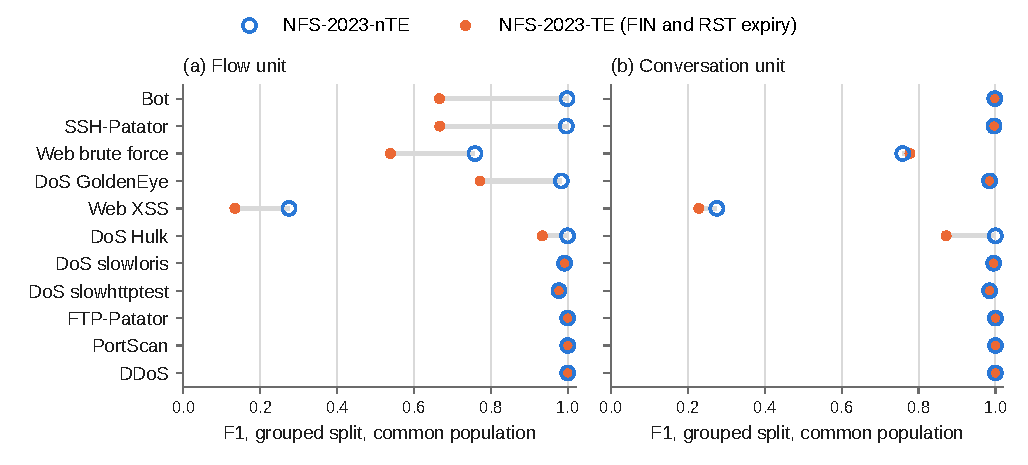
\includegraphics[width=\textwidth]{fig4_rq3_te_vs_nte.pdf}
\caption{F1 of NFS-2023-nTE and NFS-2023-TE per attack class on the common population, grouped split, mean over three models and five seeds, at the flow unit and at the conversation unit. Classes are ordered by the change at the flow unit, largest drop first; a ring and a dot that coincide mark a class the rule leaves unchanged. (a) Flow unit; (b) conversation unit}\label{fig:rq3}
\end{figure*}

\paragraph{Conversation scoring removes most of the gap, with one exception.} A second prediction, also written in advance, was that the TE minus nTE gap would be smaller at the conversation unit than at the flow unit. It is, for \RQthreeSmallerAtConv{} of the \RQthreeClasses{} classes. DoS Hulk is the exception (gap \RQthreeHulkGapFlow{} at the flow unit and \RQthreeHulkGapConv{} at the conversation unit). TE produces about \RQthreeHulkFalseTe{} benign test records per cell that models label as DoS Hulk, against about \RQthreeHulkFalseNte{} in nTE, and under the ``any'' rule each of them makes its benign conversation a false alarm. Section~\ref{sec:rq4} examines these records: they are not the smallest records of their conversations, and they occur in ordinary web connections on every capture day.

\paragraph{Leakage rises, inflation does not.} The rule lifts leakage under the random flow split from near zero to between \RQthreeLeakTeMin{} and \RQthreeLeakTeMax{} for the classes it doubles (Table~\ref{tab:rq3}). That is about what a random split with test share $q = \SetTestFrac$ gives when every conversation has two records: a test record's sibling lands in training with probability $1 - q = \SetTrainFrac$. Yet the random split gains at most \RQthreeInflMax{} F1 over the grouped split in either arm (Fig.~\ref{fig:rq3leak}): across the \RQthreeClasses{} classes the change in leakage ranges from \RQthreeDLeakMin{} to \RQthreeDLeakMax{}, and the change in this inflation from \RQthreeDInflMin{} to \RQthreeDInflMax{}. The rank correlation between the two changes is in the predicted direction but not significant (Spearman $\rho = \RQthreeRhoPooled$, one-sided permutation $p = \RQthreePPooled$), so by the rule fixed in advance the prediction is supported in direction only. Per model, $\rho$ is \RQthreeRhoRf{} for the random forest ($p = \RQthreePRf$), \RQthreeRhoLgbm{} for LightGBM ($p = \RQthreePLgbm$) and \RQthreeRhoMlp{} for the multilayer perceptron ($p = \RQthreePMlp$); on each arm's own population the pooled value is \RQthreeRhoOwn{} ($p = \RQthreePOwn$). The reason is visible in the mechanism above. A sibling record in training helps a model only if it resembles the test record, and here the two records of a conversation share almost nothing. Leakage in this sense is necessary for inflation but far from sufficient.

\begin{figure}[t]
\centering
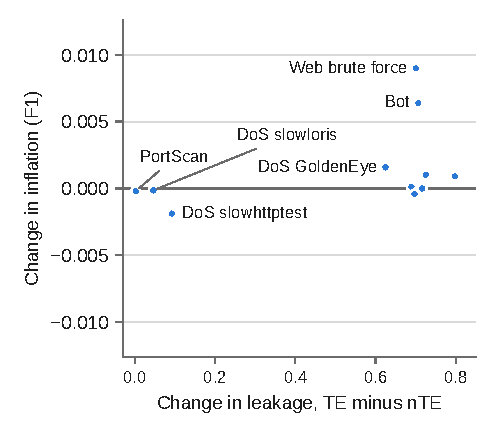
\includegraphics{fig5_rq3_leak_vs_inflation.pdf}
\caption{Change from NFS-2023-nTE to NFS-2023-TE in leakage under the random flow split (the record-level share of Table~\ref{tab:rq3}) against the change in inflation, random-split F1 minus grouped-split F1, per attack class. The unlabelled points on the right are DDoS, DoS Hulk, FTP-Patator, SSH-Patator and Web XSS}\label{fig:rq3leak}
\end{figure}

\paragraph{Answer to RQ3.} On this pair, one expiry setting changes flow-level scores by changing what the exporter puts in the test set: a featureless trailing record, which lowers the scores only because the ground truth labels it as attack. Under payload-aware labels or the releases' own labels the drop disappears. Scored per conversation, the classes it affects come back to within \RQthreeConvGapMaxOther{} F1 of their nTE values, except DoS Hulk, where the same rule creates benign records that look like the attack.

\subsection{RQ4: does conversation-level scoring restore invariance?}\label{sec:rq4}

%% RQ4 results (Phase 7). Every number is a macro from tables/numbers.tex.
Every result in this subsection comes from the setting in which the arms differ only in their exporter: the common population of conversations present in every arm, the schedule ground truth and the conversation-grouped split. The analysis plan for RQ4, with the rule for a large residual and every sensitivity variant, was committed to the repository before any RQ4 number was computed.

\paragraph{H4 is not supported, and the test cannot decide it.} Table~\ref{tab:rq4-h4} gives Kendall's $W$ of the model ranking across arms. On \cicids{} it is \RQfourWFlow{} at the flow unit and \RQfourWConv{} at the conversation unit. The difference, \RQfourDiff{} (interval \RQfourDiffLo{} to \RQfourDiffHi{}), points away from the hypothesis, but its interval includes zero, so by the rule fixed in advance H4 is not supported and is not reversed either. On UNSW-NB15, with three arms, $W$ is \RQfourWFlowUnsw{} at the flow unit and \RQfourWConvUnsw{} at the conversation unit; the difference, \RQfourDiffUnsw{} (\RQfourDiffLoUnsw{} to \RQfourDiffHiUnsw{}), also includes zero, so H4 is not supported there either. The test has little power on \cicids{} as well. With three models $W$ can take only a few values, and the multilayer perceptron ranks last in \RQtwoMlpLastArms{} arm (Section~\ref{sec:rq2}), so the rankings differ only in whether the random forest or LightGBM comes first. A high $W$ also says that the arms order the models alike, not that their scores agree. A result of ``not supported'' here is therefore not evidence that rankings fail to converge. To give the test more room we added logistic regression and a $k$-nearest-neighbour classifier, tuned and run like the other three (Section~\ref{sec:protocol}). With five models, $W$ on \cicids{} is \RevFiveWFlowCic{} at the flow unit and \RevFiveWConvCic{} at the conversation unit, and the interval of the difference, \RevFiveWDiffLoCic{} to \RevFiveWDiffHiCic{}, lies below zero: by the same rule H4 would be reversed, and the arms rank the models less alike at the conversation unit. On UNSW-NB15 $W$ is \RevFiveWFlowUnsw{} and \RevFiveWConvUnsw{} (difference \RevFiveWDiffLoUnsw{} to \RevFiveWDiffHiUnsw{}), and H4 is again not supported. This grid was added after the primary results, so it does not replace the verdict fixed in advance, but it rules out the reading that a test with more models would have shown rankings converging. The two added models also change H2. Logistic regression has the lowest macro-F1 in all \RevFiveArms{} arms of the two benchmarks, so the models now differ more, and the exporter leads for fewer classes: for \RevFiveAboveCic{} of \RevEligCic{} eligible \cicids{} classes, so H2 still holds there, but for \RevFiveAboveUnsw{} of \RevEligUnsw{} UNSW-NB15 classes, short of a strict majority (\RevFivePerdfAboveUnsw{} per degree of freedom). The exporter share is relative to the models compared, and on UNSW-NB15 the H2 verdict depends on the set of models as well as on CIC-UNSW-NB15.

% Generated by 03_Code/make_numbers.py from 04_Results/phase7/h4.csv. Do not edit by hand.
\begin{sidewaystable}
\caption{H4: Kendall's $W$ of the model ranking across arms at the flow and the conversation unit,
grouped split, common population, mean over seeds. Brackets: 95 percent cluster bootstrap intervals
(1,000 resamples of conversations). H4 predicts a positive difference (conversation minus
flow). Undecided: the interval includes zero, so H4 is not supported.}\label{tab:rq4-h4}
\small
\begin{tabularx}{\linewidth}{@{}lLllll@{}}
\toprule
Benchmark & Setting & $W$, flow & $W$, conversation & Difference & Verdict \\
\midrule
CICIDS2017 & Primary: $T = 15$ s, any rule, schedule labels & 0.886 [0.780, 0.927] & 0.820 [0.763, 0.869] & $-0.065$ [$-0.090$, 0.008] & undecided \\
 & $T = 5$ s & 0.886 [0.788, 0.910] & 0.820 [0.763, 0.861] & $-0.065$ [$-0.090$, 0.016] & undecided \\
 & $T = 30$ s & 0.886 [0.780, 0.910] & 0.820 [0.763, 0.869] & $-0.065$ [$-0.090$, 0.016] & undecided \\
 & $T = 60$ s & 0.886 [0.780, 0.918] & 0.820 [0.763, 0.870] & $-0.065$ [$-0.090$, 0.016] & undecided \\
 & $T = 120$ s & 0.886 [0.788, 0.910] & 0.820 [0.763, 0.869] & $-0.065$ [$-0.090$, 0.016] & undecided \\
 & Majority rule & 0.886 [0.780, 0.927] & 0.820 [0.771, 0.869] & $-0.065$ [$-0.090$, 0.016] & undecided \\
 & Byte-weighted rule & 0.886 [0.780, 0.927] & 0.837 [0.771, 0.878] & $-0.049$ [$-0.090$, 0.016] & undecided \\
 & Episode unit & 0.812 [0.747, 0.837] & 0.751 [0.706, 0.799] & $-0.062$ [$-0.100$, 0.005] & undecided \\
 & Attempted folded into benign (scoring only) & 0.837 [0.771, 0.861] & 0.502 [0.461, 0.551] & $-0.335$ [$-0.355$, $-0.269$] & reversed \\
 & Attempted folded into benign (retrained) & 0.616 [0.347, 0.804] & 0.535 [0.298, 0.739] & $-0.082$ [$-0.159$, 0.041] & undecided \\
 & Each release's own labels (scoring only) & 0.167 [0.151, 0.257] & 0.176 [0.143, 0.249] & 0.008 [$-0.049$, 0.024] & undecided \\
 & Each release's own labels (retrained) & 0.237 [0.131, 0.306] & 0.216 [0.110, 0.290] & $-0.020$ [$-0.078$, 0.041] & undecided \\
\midrule
UNSW-NB15 & Primary: $T = 15$ s, any rule, schedule labels & 0.867 [0.778, 0.956] & 0.822 [0.778, 0.911] & $-0.044$ [$-0.089$, 0.044] & undecided \\
 & $T = 5$ s & 0.867 [0.778, 0.911] & 0.822 [0.778, 0.911] & $-0.044$ [$-0.089$, 0.044] & undecided \\
 & $T = 30$ s & 0.867 [0.778, 0.911] & 0.822 [0.778, 0.911] & $-0.044$ [$-0.089$, 0.044] & undecided \\
 & $T = 60$ s & 0.867 [0.778, 0.911] & 0.822 [0.778, 0.911] & $-0.044$ [$-0.089$, 0.044] & undecided \\
 & $T = 120$ s & 0.867 [0.778, 0.956] & 0.822 [0.778, 0.911] & $-0.044$ [$-0.089$, 0.044] & undecided \\
 & Majority rule & 0.867 [0.778, 0.956] & 0.822 [0.778, 0.911] & $-0.044$ [$-0.133$, 0.044] & undecided \\
 & Byte-weighted rule & 0.867 [0.778, 0.956] & 0.822 [0.778, 0.911] & $-0.044$ [$-0.089$, 0.044] & undecided \\
 & Episode unit & 0.822 [0.778, 0.868] & 0.822 [0.778, 0.867] & 0.000 [$-0.044$, 0.044] & undecided \\
 & Each release's own labels (scoring only) & 0.867 [0.778, 0.956] & 0.867 [0.778, 0.956] & 0.000 [$-0.044$, 0.089] & undecided \\
\bottomrule
\end{tabularx}
\end{sidewaystable}


\paragraph{Definition~\ref{def:invariance} tested directly.} H4 asks whether the arms order the models alike; Definition~\ref{def:invariance} asks whether a metric has the same value whatever the exporter. We test that directly on the common population with two one-sided tests: for each model, class with enough test conversations in every arm, and pair of arms, the per-class F1 of the two arms, averaged over seeds, is called equivalent at margin $\delta$ when the \setnum{90} percent cluster bootstrap interval of its difference lies inside $(-\delta, \delta)$. We report $\delta = \setnum{0.01}$, the margin of the RQ5 claims of no difference, \setnum{0.02} and \setnum{0.05}, a difference most papers would report as an improvement. Over the \RevEqTestsCic{} tests on \cicids{}, \RevEqCicFlowTwo{} percent are equivalent at \setnum{0.02} at the flow unit and \RevEqCicConvTwo{} percent at the conversation unit, and \RevEqCicFlowFive{} and \RevEqCicConvFive{} percent at \setnum{0.05}. For macro-F1 over the fixed classes the share at \setnum{0.05} rises from \RevEqMacCicFlowFive{} to \RevEqMacCicConvFive{} percent. On UNSW-NB15, over \RevEqTestsUnsw{} tests, the shares are much lower: \RevEqUnswFlowFive{} percent at the flow unit and \RevEqUnswConvFive{} percent at the conversation unit at \setnum{0.05}, and no macro-F1 comparison is equivalent at \setnum{0.02} at either unit. So the conversation unit moves both benchmarks towards invariance, but by Definition~\ref{def:invariance} neither metric is exporter invariant on either benchmark: even at the conversation unit, the comparisons not counted above, a minority on \cicids{} and most on UNSW-NB15, cannot be shown to differ by less than \setnum{0.05}.

\paragraph{The conversation unit removes most of the exporter share, but not all of it.} The exporter share of the variance in per-class F1 tells more than the ranking does. From the flow unit to the conversation unit it falls, with an interval that excludes zero, for \RQfourShareFallsCic{} of the \RQfourShareOfCic{} \cicids{} classes with enough test conversations, benign included: SSH-Patator goes from \RQfourSshShareFlow{} to \RQfourSshShareConv{}, DoS GoldenEye from \RQfourGoldenShareFlow{} to \RQfourGoldenShareConv{} and Bot from \RQfourBotShareFlow{} to \RQfourBotShareConv{}. This is what the RQ3 mechanism predicts, since scoring each conversation once removes the weight that tail records add. For \RQfourShareRisesCic{} classes the share rises: DoS Hulk from \RQfourHulkShareFlow{} to \RQfourHulkShareConv{} and FTP-Patator from \RQfourFtpShareFlow{} to \RQfourFtpShareConv{}. On UNSW-NB15 the share falls for \RQfourShareFallsUnsw{} of \RQfourShareOfUnsw{} classes, most for Generic, from \RQfourGenericShareFlow{} to \RQfourGenericShareConv{}. At the conversation unit the exporter leads for only \RQfourUnswConvAbove{} of the \RQfourUnswConvElig{} eligible UNSW-NB15 classes, so on that benchmark H2 holds at the flow unit and not at the conversation unit.

\paragraph{What remains.} We call a residual large when the exporter share at the conversation unit is at least \setnum{0.25} and the arm means of F1 spread by at least \setnum{0.05}. Table~\ref{tab:rq4-residual} lists the \RQfourLargeCic{} \cicids{} classes and \RQfourLargeUnsw{} UNSW-NB15 classes that meet both conditions.

% Generated by 03_Code/make_numbers.py from 04_Results/phase7/residual.csv. Do not edit by hand.
\begin{table}[t]
\caption{Classes with a large residual exporter effect at the conversation unit (grouped split,
common population): exporter share of the variance in per-class F1 at least \setnum{0.25} and a
spread of arm means of F1 of at least \setnum{0.05}. Brackets: 95 percent cluster bootstrap
intervals. Last column: the two arms with the lowest mean F1 over three models and five
seeds.}\label{tab:rq4-residual}
\small
\begin{tabularx}{\linewidth}{@{}lllL@{}}
\toprule
Class & Exporter share & Spread & Lowest arms (mean F1) \\
\midrule
\multicolumn{4}{@{}l}{\emph{\cicids}} \\
FTP-Patator & 0.966 [0.949, 0.973] & 0.085 & CIC original 0.915; BCCC 0.972 \\
DoS Hulk & 0.722 [0.708, 0.734] & 0.128 & NFS-2023-TE 0.872; BCCC 0.945 \\
Bot & 0.559 [0.508, 0.587] & 0.070 & BCCC 0.929; CIC original 0.944 \\
SSH-Patator & 0.301 [0.292, 0.309] & 0.065 & BCCC 0.933; CIC original 0.994 \\
\midrule
\multicolumn{4}{@{}l}{\emph{UNSW-NB15}} \\
Fuzzers & 0.841 [0.810, 0.855] & 0.067 & CIC-UNSW-NB15 0.797; UNSW-NB15 original, duplicates dropped 0.851 \\
Shellcode & 0.788 [0.752, 0.818] & 0.467 & CIC-UNSW-NB15 0.366; UNSW-NB15 original, duplicates dropped 0.658 \\
Exploits & 0.571 [0.525, 0.601] & 0.050 & CIC-UNSW-NB15 0.820; UNSW-NB15 original, duplicates dropped 0.848 \\
Analysis & 0.479 [0.274, 0.587] & 0.162 & NF-UNSW-NB15-v3 0.202; CIC-UNSW-NB15 0.243 \\
Worms & 0.329 [0.234, 0.393] & 0.267 & UNSW-NB15 original, duplicates dropped 0.426; CIC-UNSW-NB15 0.484 \\
DoS & 0.280 [0.241, 0.313] & 0.136 & CIC-UNSW-NB15 0.399; UNSW-NB15 original, duplicates dropped 0.420 \\
Generic & 0.272 [0.244, 0.299] & 0.118 & CIC-UNSW-NB15 0.751; UNSW-NB15 original, duplicates dropped 0.769 \\
\bottomrule
\end{tabularx}
\end{table}


On \cicids{} the residual has one cause, and it is the mirror image of RQ3. For the four classes, recall is at least \RQfourResRecallMin{} in every arm. What falls is precision, and only in the three arms that write tail records: CIC original, BCCC and NFS-2023-TE. In the other four arms precision stays at \RQfourPrecOtherMin{} or above. Almost every false positive in the three tail arms is a benign conversation with two or more records, exactly one of which the model assigned to the attack class: \RQfourFpOneFtp{} of \RQfourFpFtp{} FTP-Patator false positives in CIC original, \RQfourFpOneSsh{} of \RQfourFpSsh{} SSH-Patator false positives in BCCC, \RQfourFpOneBot{} of \RQfourFpBot{} Bot false positives in BCCC, and \RQfourFpOneHulk{} of \RQfourFpHulk{} DoS Hulk false positives in NFS-2023-TE (counts summed over three models and five seeds). BCCC DoS Hulk differs in degree: \RQfourFpMultiHulkBccc{} of its \RQfourFpHulkBccc{} false positives are benign conversations with several records, but only \RQfourFpOneHulkBccc{} have exactly one record flagged. The schedule labels the tail record of an attack conversation as the attack, because a record inherits the label of its conversation. A model trained on these labels learns that a short end-of-connection record belongs to the attack class, and the same kind of record at the end of a benign connection then raises an alert, which the ``any'' rule turns into a false alarm for the whole conversation. In a spot check made by hand from the stored predictions and not part of the scripted pipeline (one model and seed per class), the flagged record in CIC original and BCCC was in most cases the smallest record of its conversation, with zero bytes in the release; we report it as an unscripted observation.

NFS-2023-TE DoS Hulk is only partly explained. Its flagged records are not the smallest of their conversations, and the conversations are ordinary web connections to many external hosts on every capture day, Monday included, which has no attack, so they are not mislabelled attack traffic. A record that TE writes in benign web connections resembles the records TE writes for DoS Hulk; which expiry rule produces it we have not confirmed. This is the same set of benign records as in RQ3 (Section~\ref{sec:rq3}).

On UNSW-NB15 the residual comes mostly from CIC-UNSW-NB15, and it is not the \cicids{} pattern. CIC-UNSW-NB15 has the lowest mean F1 of the three arms in \RQfourUnswCicLowestFone{} of the \RQfourLargeUnsw{} classes and the lowest recall in \RQfourUnswCicLowestRecall{}. In that release \RQfourUnswCicMultiMin{} to \RQfourUnswCicMultiMax{} percent of the conversations of these classes have several records, against at most \RQfourUnswOtherMultiMax{} percent in the other two, and only \RQfourUnswCicFnBenign{} percent of the attack conversations it misses are called benign: the models confuse attack classes with each other rather than with benign traffic. Whether the split records cause these confusions, or the CICFlowMeter features of a split record, we did not test. The original and NF-UNSW-NB15-v3 also differ in their feature sets, the Argus and Bro features against the NetFlow fields, and which features matter we did not test either.

Three checks support the reading for \cicids{}. Under the payload-aware labels of Section~\ref{sec:rq3}, which call records without payload benign in training and test, \RevPayLarge{} \cicids{} classes have a large residual, against \RevSchLarge{} under the schedule, and no attack class spreads by more than \RevPaySpreadMax{} F1 across arms at the conversation unit. $W$ under these labels is \RevPayWFlow{} at the flow unit and \RevPayWConv{} at the conversation unit (difference interval \RevPayWDiffLo{} to \RevPayWDiffHi{}), so H4 is not supported there either. Under the byte-weighted rule, which assigns a conversation the class of its records with the most bytes and so ignores an empty tail, \RQfourBytesLarge{} \cicids{} classes have a large residual and the arm means of the four classes spread by at most \RQfourBytesSpreadMax{}. Leaving out the arm that writes the tails lowers the residual share (point estimates, no intervals): for SSH-Patator from \RQfourSshShareConv{} to \RQfourLoaoSshBccc{} without BCCC, and for DoS Hulk from \RQfourHulkShareConv{} to \RQfourLoaoHulkTe{} without NFS-2023-TE. For FTP-Patator, leaving out CIC original lowers it only to \RQfourLoaoFtpOrig{}, because BCCC writes the same tails.

\paragraph{Sensitivity.} Table~\ref{tab:rq4-sens} states, for each of the \RQfourSensVariants{} \cicids{} variants, which conclusions change. Five conclusions are tracked: H4, H2 at the flow unit, H2 at the conversation unit, the per-class verdict of exporter against model at the conversation unit, and the direction in which the exporter share moves from flow to conversation. H4 changes under \RQfourSensChangedHfour{} variant, H2 at the flow unit under \RQfourSensChangedHtwoFlow{} and H2 at the conversation unit under \RQfourSensChangedHtwoConv{}. Class verdicts change for at most \RQfourSensKfourMax{} of \RQfourClassesOf{} classes, and share directions for at most \RQfourSensKfiveMax{}. On UNSW-NB15, H2 holds at the flow unit and not at the conversation unit in every variant except scoring against each release's own labels, under which the exporter leads at the flow unit for only \RQfourUnswOwnAbove{} of \RQfourUnswOwnElig{} classes and H2 does not hold there either.

% Generated by 03_Code/make_numbers.py from 04_Results/phase7/sensitivity_table.csv. Do not edit by hand.
\begin{sidewaystable}
\caption{What each sensitivity setting changes. H4: the difference in Kendall's $W$, conversation
minus flow, with its interval. H2 at the flow and the conversation unit. Class verdicts: how many
classes change their exporter-against-model verdict at the conversation unit (grouped split, common
population). Share direction: how many classes change the direction in which the exporter share
moves from the flow to the conversation unit. A class whose verdict becomes not estimable is not
counted as a change. Changed: the conclusions that differ from the primary setting.}\label{tab:rq4-sens}
\small
\setlength{\tabcolsep}{4pt}
\begin{tabularx}{\linewidth}{@{}lLlllrrl@{}}
\toprule
 & & & \multicolumn{2}{c}{H2} & Class & Share & \\
\cmidrule(lr){4-5}
Benchmark & Setting & H4 difference & Flow & Conversation & verdicts & direction & Changed \\
\midrule
CICIDS2017 & Primary: $T = 15$ s, any rule, schedule labels & $-0.065$ [$-0.090$, 0.008] & holds & holds & 0 of 12 & 0 of 12 & none \\
 & $T = 5$ s & $-0.065$ [$-0.090$, 0.016] & holds & holds & 1 of 12 & 0 of 12 & none \\
 & $T = 30$ s & $-0.065$ [$-0.090$, 0.016] & holds & holds & 0 of 12 & 0 of 12 & none \\
 & $T = 60$ s & $-0.065$ [$-0.090$, 0.016] & holds & holds & 0 of 12 & 1 of 12 & none \\
 & $T = 120$ s & $-0.065$ [$-0.090$, 0.016] & holds & holds & 0 of 12 & 0 of 12 & none \\
 & Majority rule & $-0.065$ [$-0.090$, 0.016] & holds & holds & 3 of 12 & 2 of 12 & none \\
 & Byte-weighted rule & $-0.049$ [$-0.090$, 0.016] & holds & does not hold & 4 of 12 & 2 of 12 & H2 conv. \\
 & Episode unit & $-0.062$ [$-0.100$, 0.005] & not estimable & not estimable & 0 of 12 & 1 of 12 & none \\
 & Attempted folded into benign (scoring only) & $-0.335$ [$-0.355$, $-0.269$] & holds & holds & 0 of 12 & 1 of 12 & H4 \\
 & Attempted folded into benign (retrained) & $-0.082$ [$-0.159$, 0.041] & holds & holds & 2 of 12 & 2 of 12 & none \\
 & Each release's own labels (scoring only) & 0.008 [$-0.049$, 0.024] & holds & holds & 2 of 12 & 7 of 12 & none \\
 & Each release's own labels (retrained) & $-0.020$ [$-0.078$, 0.041] & holds & holds & 2 of 12 & 9 of 12 & none \\
\midrule
UNSW-NB15 & Primary: $T = 15$ s, any rule, schedule labels & $-0.044$ [$-0.089$, 0.044] & holds & does not hold & 0 of 10 & 0 of 10 & none \\
 & $T = 5$ s & $-0.044$ [$-0.089$, 0.044] & holds & does not hold & 0 of 10 & 0 of 10 & none \\
 & $T = 30$ s & $-0.044$ [$-0.089$, 0.044] & holds & does not hold & 0 of 10 & 0 of 10 & none \\
 & $T = 60$ s & $-0.044$ [$-0.089$, 0.044] & holds & does not hold & 0 of 10 & 0 of 10 & none \\
 & $T = 120$ s & $-0.044$ [$-0.089$, 0.044] & holds & does not hold & 0 of 10 & 0 of 10 & none \\
 & Majority rule & $-0.044$ [$-0.133$, 0.044] & holds & does not hold & 2 of 10 & 5 of 10 & none \\
 & Byte-weighted rule & $-0.044$ [$-0.089$, 0.044] & holds & does not hold & 1 of 10 & 0 of 10 & none \\
 & Episode unit & 0.000 [$-0.044$, 0.044] & holds & does not hold & 1 of 10 & 1 of 10 & none \\
 & Each release's own labels (scoring only) & 0.000 [$-0.044$, 0.089] & does not hold & does not hold & 2 of 10 & 1 of 10 & H2 flow \\
\bottomrule
\end{tabularx}
\end{sidewaystable}


The gap $T$ does not matter between \NsweepCicStableMin{} and \setnum{120} seconds: each of the four alternative values changes at most \RQfourSensTClassMax{} class verdict or share direction, and no hypothesis verdict. The aggregation rule matters for the residual and not for H4. The byte-weighted rule removes the \cicids{} residual, as above, and with it the exporter's lead at the conversation unit, so H2 at that unit no longer holds; majority voting keeps the residual, because most of these conversations have two records and a tie goes to the attack class. An evaluator who scores per conversation therefore has to state the rule.

Folding attempted attacks into benign at test time, with models trained on the primary labels, is the one variant that reverses H4 (difference \RQfourFoldScoreDiff{}, interval \RQfourFoldScoreDiffLo{} to \RQfourFoldScoreDiffHi{}). This variant scores the models as wrong for calling attempts attacks, which they were trained to do. Retrained on the folded labels, the reversal is gone: the difference is \RQfourFoldRetrDiff{} (\RQfourFoldRetrDiffLo{} to \RQfourFoldRetrDiffHi{}), undecided as in the primary setting, and \RQfourFoldRetrainedClasses{} class verdicts change. We read the reversal as a product of scoring against labels the models did not learn.

Scored against each release's own labels instead of the schedule, the arms nearly stop agreeing on the model ranking: $W$ at the flow unit is \RQfourOwnScoreWFlow{}, against \RQfourWFlow{} with the schedule truth. Retrained and scored on their own labels, as a user of one release alone would work, the arms give $W$ of \RQfourOwnRetrWFlow{} at the flow unit and \RQfourOwnRetrWConv{} at the conversation unit (difference \RQfourOwnRetrDiff{}, interval \RQfourOwnRetrDiffLo{} to \RQfourOwnRetrDiffHi{}). H2 still holds, for \RQfourOwnRetrHtwoAbove{} of \RQfourOwnRetrHtwoElig{} eligible classes, but the share direction changes for \RQfourOwnRetrKfive{} of \RQfourClassesOf{} classes. The fall in the exporter share from flow to conversation unit therefore belongs to the setting with one ground truth, and the labels are a second channel through which a release changes scores, which the schedule truth closes by design.

\paragraph{Episodes are not a usable unit on \cicids{}.} An episode groups the attack conversations of one class between one pair of hosts: on \cicids{} within one window of the attack schedule, and on UNSW-NB15, which has no schedule windows, as long as consecutive conversations start at most \setnum{300} seconds after the previous ones end. Episodes were frozen with the instrument and are scored here as a sensitivity unit. On \cicids{} each attack class has at most \RQfourEpisodeMax{} test episodes (\RQfourEpisodeMaxClass{}), and in every seed every attack episode has conversations on both sides of the conversation-grouped split. Claims at the level of an attack campaign cannot be tested on this benchmark, and the conversation split is not independent at that level. On UNSW-NB15 episodes are numerous, but many straddle the split too: \RQfourEpisodeStradDos{} percent of DoS test episodes and \RQfourEpisodeStradExploits{} percent of Exploits test episodes, depending on the seed.

\paragraph{Answer to RQ4.} Conversation-level scoring with conversation-grouped splits does not make model rankings more consistent across exporters. H4 was not supported by the test fixed in advance, with intervals that include zero; with five models the difference on \cicids{} lies below zero, so rankings agree less at the conversation unit, and with three models it reversed when attempted attacks were relabelled benign at test time without retraining. The scoring unit does remove most of the exporter's share of per-class F1 on \cicids{} and raises the share of between-release comparisons that are equivalent within \setnum{0.05}, but it does not make F1 exporter invariant in the sense of Definition~\ref{def:invariance}. What remains on \cicids{} has one identified cause, a short end-of-connection record that the schedule labels as the attack in attack conversations and that makes benign conversations false alarms; a byte-weighted rule or payload-aware labels remove it. On UNSW-NB15 the conversation unit also removes most of the exporter's lead, and the residual that remains in \RQfourLargeUnsw{} classes comes mostly from CIC-UNSW-NB15, through attacks confused with other attack classes, a kind we have not explained.


\subsection{RQ5: which published claims survive}\label{sec:rq5}

%% RQ5 results (Phase 8). Every number is a macro from tables/numbers.tex.
We re-examined five published comparisons of releases (Section~\ref{sec:claims}): Rosay et al.\ on LYCOS-IDS2017 against the original \cicids{} (R1) \cite{rosay2021}, Engelen et al.\ on WTMC-2021 (R2) \cite{engelen2021}, Lanvin et al.\ on the CRiSIS-2022 variants (R3) \cite{lanvin2023}, Sarhan et al.\ on the NetFlow version of UNSW-NB15 (R4) \cite{sarhan2022} and Pekar and Jozsa on five releases per day (R5) \cite{pekar2024}. They give \RQfiveRows{} headline contrasts, listed in Table~\ref{tab:rq5} and drawn in Fig.~\ref{fig:rq5}. Each contrast is examined in three steps: the per-flow comparison rebuilt the way the authors made it, a decomposition of that per-flow gap, and the same contrast on conversations present in both releases, with one ground truth, the conversation-grouped split and conversation scoring.

% Generated by 03_Code/make_numbers.py from 04_Results/phase8/verdicts_sched.csv. Do not edit by hand.
\begin{sidewaystable}
\caption{Published claims that one release is better than another. Contrast: release B vs release
A; every gap is B minus A in the claim's metric (F1, recall and MCC without a class: attack against
benign). R5: (a) Tuesday, each refined release against CIC original; (b) Thursday; (c) the claim
of no difference, NFS-2023-TE against NFS-2023-nTE on each day. Published: the gap the authors
report. Per flow, as published: our rebuild of their comparison. Per flow, shared conv.: the
rebuilt per-flow comparison restricted to the conversations present in both releases, with schedule
labels and the grouped split. Per conversation: the same comparison scored once per conversation;
the verdict is read from this column. Attempts benign: the verdict when attempted attacks are folded
into benign (Section~\ref{sec:gt}); n/a, UNSW-NB15 has no attempted attacks; not computed, the
contrast involves no class with attempted attacks, or was not rerun. R4: the per-flow rebuild uses
NF-UNSW-NB15-v2 itself and, on the second line, NF-UNSW-NB15-v3; the shared-conversation and
conversation-level contrasts use NF-UNSW-NB15-v3, which has the timestamps that v2 lacks.
Prevalence: the published and per-flow gaps use each release's test data as the authors split it;
the shared-conversation and per-conversation gaps use the subsample of Section~\ref{sec:protocol},
in which attacks are more prevalent. Recall (R3, and R4 Fuzzers and Worms) does not depend on class
prevalence; F1 and MCC do. R1 models: RF random forest, DT decision tree, LDA linear
discriminant analysis. Brackets: 95 percent paired cluster bootstrap intervals over conversations.
Verdicts: zero by construction, the two releases are one arm under schedule labels; data not
obtained, the release could not be downloaded. R5 rows name the capture day after the
metric.}\label{tab:rq5}
\footnotesize
\setlength{\tabcolsep}{3pt}
\begin{tabularx}{\linewidth}{@{}Llr*{3}{>{\raggedright\arraybackslash}p{2.4cm}}*{2}{>{\raggedright\arraybackslash}p{1.6cm}}@{}}
\toprule
Contrast & Metric & Published & Per flow, as published & Per flow, shared conv. & Per conversation & Verdict & Attempts benign \\
\midrule
\multicolumn{8}{@{}l}{\emph{R1, Rosay et al.}} \\
LYCOS vs CIC original, RF & MCC & 0.001 & 0.001 [0.001, 0.001] & 0.002 [0.001, 0.002] & 0.001 [0.000, 0.001] & survives & not computed \\
LYCOS vs CIC original, DT & MCC & 0.001 & 0.001 [0.000, 0.001] & 0.001 [0.001, 0.001] & 0.001 [0.001, 0.001] & survives & not computed \\
LYCOS vs CIC original, LDA & MCC & 0.155 & 0.155 [0.152, 0.158] & 0.210 [0.207, 0.213] & 0.164 [0.162, 0.167] & survives & not computed \\
\addlinespace
\multicolumn{8}{@{}l}{\emph{R2, Engelen et al.}} \\
WTMC-2021 vs CIC original & F1, Bot & 0.390 & 0.183 [0.168, 0.199] & 0.048 [0.039, 0.057] & 0.030 [0.021, 0.040] & survives & survives \\
WTMC-2021 vs CIC original & F1, Web brute force & 0.180 & 0.222 [0.186, 0.251] & 0.013 [0.000, 0.026] & $-0.040$ [$-0.055$, $-0.027$] & reverses & not supported \\
WTMC-2021 vs CIC original & F1, Web XSS & 0.610 & 0.458 [0.254, 0.586] & 0.040 [0.004, 0.072] & 0.197 [0.153, 0.239] & survives & not estimable \\
WTMC-2021 vs CIC original & F1, Infiltration & 0.100 & 0.190 [0.063, 0.424] & n/a & n/a & not estimable & not estimable \\
WTMC-2021 vs CIC original & F1, Heartbleed & 0.160 & 0.040 [0.040, 0.040] & n/a & n/a & not estimable & not estimable \\
WTMC-2021 vs CIC original & F1, Web SQL injection & $-0.110$ & 0.214 [$-0.138$, 0.500] & 0.043 [$-0.237$, 0.241] & $-0.234$ [$-0.505$, $-0.027$] & not estimable & not estimable \\
\addlinespace
\multicolumn{8}{@{}l}{\emph{R3, Lanvin et al.}} \\
CRiSIS-2022 Exp\_RP vs CRiSIS-2022 Exp\_RPD & Recall & 0.200 & 0.211 [0.209, 0.212] & 0.000 [0.000, 0.000] & 0.000 [0.000, 0.000] & not supported & survives \\
CRiSIS-2022 Exp\_RP vs CRiSIS-2022 Exp\_RPD & Recall & 0.000 & $-0.006$ [$-0.006$, $-0.006$] & 0.000 [0.000, 0.000] & 0.000 [0.000, 0.000] & survives & survives \\
CRiSIS-2022 Exp\_RPD vs CRiSIS-2022 Exp\_RD & Recall & $-0.200$ & $-0.217$ [$-0.218$, $-0.215$] & 0.000 [0.000, 0.000] & 0.000 [0.000, 0.000] & zero by construction & zero by construction \\
\bottomrule
\end{tabularx}
\end{sidewaystable}

\begin{sidewaystable}
\addtocounter{table}{-1}
\renewcommand{\theHtable}{\arabic{table}.cont}
\caption{Published claims that one release is better than another (continued).}
\footnotesize
\setlength{\tabcolsep}{3pt}
\begin{tabularx}{\linewidth}{@{}Llr*{3}{>{\raggedright\arraybackslash}p{2.4cm}}*{2}{>{\raggedright\arraybackslash}p{1.6cm}}@{}}
\toprule
Contrast & Metric & Published & Per flow, as published & Per flow, shared conv. & Per conversation & Verdict & Attempts benign \\
\midrule
\multicolumn{8}{@{}l}{\emph{R4, Sarhan et al.}} \\
NF-UNSW-NB15-v3 vs UNSW-NB15 original & F1 & 0.050 & v2 $-0.009$ [$-0.016$, 0.004]\newline v3 0.022 [0.016, 0.036] & $-0.019$ [$-0.031$, 0.013] & $-0.003$ [$-0.004$, $-0.002$] & reverses & n/a \\
NF-UNSW-NB15-v3 vs UNSW-NB15 original & Recall, Fuzzers & 0.301 & v2 0.254 [0.214, 0.296]\newline v3 0.267 [0.226, 0.311] & $-0.022$ [$-0.027$, $-0.016$] & $-0.019$ [$-0.024$, $-0.013$] & reverses & n/a \\
NF-UNSW-NB15-v3 vs UNSW-NB15 original & Recall, Worms & 0.807 & v2 0.672 [0.613, 0.734]\newline v3 0.608 [0.520, 0.692] & 0.685 [0.594, 0.763] & 0.685 [0.593, 0.763] & survives & n/a \\
\addlinespace
\multicolumn{8}{@{}l}{\emph{R5, Pekar and Jozsa}} \\
(a) WTMC-2021 vs CIC original & F1, Tuesday & 0.129 & 0.129 [0.122, 0.136] & 0.105 [0.101, 0.108] & 0.106 [0.100, 0.111] & survives & not computed \\
(a) CRiSIS-2022 Exp\_RP vs CIC original & F1, Tuesday & 0.128 & 0.129 [0.122, 0.136] & 0.105 [0.101, 0.109] & 0.105 [0.100, 0.111] & survives & not computed \\
(a) NFS-2023-nTE vs CIC original & F1, Tuesday & 0.128 & 0.128 [0.122, 0.136] & 0.105 [0.101, 0.109] & 0.104 [0.098, 0.110] & survives & not computed \\
(a) NFS-2023-TE vs CIC original & F1, Tuesday & 0.128 & 0.129 [0.122, 0.136] & $-0.013$ [$-0.017$, $-0.009$] & 0.104 [0.098, 0.110] & survives & not computed \\
(b) NFS-2023-nTE vs NFS-2023-TE & F1, Thursday & 0.050 & 0.050 [0.047, 0.052] & 0.177 [0.168, 0.186] & 0.292 [0.279, 0.305] & survives & not computed \\
(b) CRiSIS-2022 Exp\_RP vs WTMC-2021 & F1, Thursday & 0.047 & 0.047 [0.008, 0.099] & 0.000 [$-0.001$, 0.001] & 0.000 [$-0.001$, 0.001] & not supported & not computed \\
(b) NFS-2023-nTE vs CIC original & F1, Thursday & 0.051 & 0.050 [0.037, 0.064] & 0.033 [0.028, 0.037] & 0.015 [0.010, 0.020] & survives & not computed \\
(c) NFS-2023-TE vs NFS-2023-nTE & F1, Tuesday & 0.000 & 0.000 [$-0.001$, 0.001] & $-0.118$ [$-0.120$, $-0.116$] & 0.000 [$-0.001$, 0.000] & survives & not computed \\
(c) NFS-2023-TE vs NFS-2023-nTE & F1, Wednesday & 0.000 & 0.000 [0.000, 0.000] & $-0.044$ [$-0.045$, $-0.042$] & $-0.022$ [$-0.023$, $-0.021$] & contradicted & not computed \\
(c) NFS-2023-TE vs NFS-2023-nTE & F1, Thursday & $-0.050$ & $-0.050$ [$-0.052$, $-0.047$] & $-0.177$ [$-0.186$, $-0.168$] & $-0.292$ [$-0.305$, $-0.279$] & contradicted & not computed \\
(c) NFS-2023-TE vs NFS-2023-nTE & F1, Friday & 0.000 & 0.000 [0.000, 0.000] & $-0.006$ [$-0.006$, $-0.006$] & 0.000 [0.000, 0.000] & survives & not computed \\
\bottomrule
\end{tabularx}
\end{sidewaystable}


\paragraph{The per-flow rebuilds reproduce most published gaps.} Where we could follow the authors' code, the rebuild lands on their numbers: for R1 and R5 every rebuilt score is within \RQfiveFidelityMax{} of the published one. R3 reproduces the published fall in recall when the corrected labels are used (\RQfiveQtwoFlow{} against about \RQfiveQtwoPub{}). Two rebuilds differ on one side. In R2 our scores on WTMC-2021 are close to the published ones, but on the original release they are higher (Bot F1 \RQfiveRtwoBotOrigOurs{} against \RQfiveRtwoBotOrigPub{}), so the rebuilt gap is smaller (Bot \RQfiveBotFlow{} against \RQfiveBotPub{}); we did not read the authors' hyperparameters or feature list, which is the likely source. In R4 our binary F1 on the original UNSW-NB15 is \RQfiveRfourOrigOurs{} against a published \RQfiveRfourOrigPub{}, while the NetFlow side matches, so the published binary advantage is not reproduced (gap \RQfiveBinFlow{}, interval \RQfiveBinFlowLo{} to \RQfiveBinFlowHi{}); the per-class gain for Fuzzers is reproduced (\RQfiveFuzzFlow{} against \RQfiveFuzzPub{}). Every deviation from the authors' setups is ours and is listed with the code. Where a rebuild does not reproduce the published baseline, a changed verdict could come from the rebuild rather than from the scoring unit. Table~\ref{tab:rq5} therefore gives, beside the conversation-level gap, the rebuilt per-flow gap restricted to the shared conversations with one truth. Comparing it with the per-flow gap as published separates what changes with the population and the labels from what changes with the unit, within the same rebuild.

\paragraph{Class weights never explain a whole gap.} A per-flow gap between two releases splits into a class weight part, from the change in how many test records each class has, a within-class part, and a part from classes that only one release has. The class weight part is small and mostly negative in R2 (Bot \RQfiveBotC{}, Web XSS \RQfiveXssC{}, Web brute force \RQfiveWebBfC{}) and is zero by design in R1, whose test sets hold equal numbers of attack records per class. In R3 it is \RQfiveQtwoC{} of the \RQfiveQtwoFlow{} gap, the rest within class (\RQfiveQtwoW{}); the flows of the two releases are the same, and what changes is which test records count as attacks. In R4 the two parts have opposite signs (class weights \RQfiveBinC{}, within class \RQfiveBinW{}). The largest structural effect is in R5 on Thursday, where NFS-2023-nTE beats CIC original by \RQfiveThuNteCicPub{} as published. The classes both releases share contribute \RQfiveThuNteCicShared{} to that gap (class weights \RQfiveThuNteCicC{}, within class \RQfiveThuNteCicW{}), and the port scan that NFS-2023-nTE labels on Thursday, a class the original release does not have on that day, contributes \RQfiveThuNteCicNonshared{}. The published advantage comes from labelling an easy class, not from better detection of the classes both releases share.

\paragraph{Verdicts per conversation.} Of the \RQfiveRows{} contrasts, \RevFiveUndecided{} cannot be decided on the same conversations with one truth: \RQfiveNotEstimable{} are not estimable because a class has fewer than \SetMinTest{} test conversations, and \RQfiveZero{} is zero by construction. Of the \RevFiveDecided{} that can be decided, \RQfiveSurvive{} survive (\RevFiveSurvivePct{} percent), \RQfiveReverse{} reverse, \RQfiveContradicted{} claims of no difference are contradicted and \RQfiveNotSupported{} are not supported. The verdict rules were fixed before any conversation-level number was computed: a claim survives when the gap has the published sign and its interval excludes zero, reverses when the interval lies entirely on the other side, and is not supported when the interval includes zero; a claim of no difference survives when the interval lies within \setnum{0.01} of zero and is contradicted when it excludes zero.

Where a claim survives, its size often shrinks. In R1 the LYCOS advantage for linear discriminant analysis holds (\RQfiveLdaConv{}, interval \RQfiveLdaConvLo{} to \RQfiveLdaConvHi{}, against \RQfiveLdaPub{} published). In R2 the WTMC-2021 gain for Bot falls from \RQfiveBotPub{} published to \RQfiveBotConv{} (\RQfiveBotConvLo{} to \RQfiveBotConvHi{}), and for Web XSS from \RQfiveXssPub{} to \RQfiveXssConv{}. The R2 gain for Web brute force reverses (\RQfiveWebBfConv{}, \RQfiveWebBfConvLo{} to \RQfiveWebBfConvHi{}), but this verdict depends on how attempted attacks are labelled: with attempts folded into benign the gap is \RQfiveFoldWebBfConv{} (\RQfiveFoldWebBfConvLo{} to \RQfiveFoldWebBfConvHi{}) and the claim is \RQfiveFoldWebBfVerdict{}, while Bot still \RQfiveFoldBotVerdict{} and Web XSS becomes \RQfiveFoldXssVerdict{}. Infiltration, Heartbleed and Web SQL injection are not estimable in R2.

R3 compares releases that differ only in labels. Under one schedule truth the corrected release and the release it corrects become the same arm, so their gap is zero by construction; the claim cannot be tested this way, and the per-flow result above is the finding. The two R3 contrasts that involve Exp\_RP, the variant without duplicated packets, show the same thing from the other side. Per flow, Exp\_RP raises recall over Exp\_RPD by \RQfiveQthreeFlow{} (\RQfiveQthreeFlowLo{} to \RQfiveQthreeFlowHi{}), close to the published \RQfiveQthreePub{}. Per conversation the gain is \RQfiveQthreeConv{} (\RQfiveQthreeConvLo{} to \RQfiveQthreeConvHi{}): both releases detect about \RQfiveQthreeRecall{} percent of attack conversations, so the published gain comes from how records are counted and labelled, not from what is detected, and the claim is not supported. The claim that Exp\_RD and Exp\_RP give the same recall survives (\RQfiveQfourFlow{} per flow, \RQfiveQfourConv{} per conversation).

R4 changes most. NF-UNSW-NB15-v2 has no timestamps, so it cannot be put on our clock, and the conversation-level contrast uses NF-UNSW-NB15-v3, the same feature set with millisecond timestamps, in its place. On the same conversations, the NetFlow arm is not better at binary detection (\RQfiveBinConv{}, \RQfiveBinConvLo{} to \RQfiveBinConvHi{}, against \RQfiveBinPub{} published) and is worse on Fuzzers (\RQfiveFuzzConv{}, \RQfiveFuzzConvLo{} to \RQfiveFuzzConvHi{}, against \RQfiveFuzzPub{}); only Worms keeps a large gain (\RQfiveWormsConv{}, \RQfiveWormsConvLo{} to \RQfiveWormsConvHi{}, against \RQfiveWormsPub{}). The proxy matters for the binary row. Per flow, NF-UNSW-NB15-v3 beats the original by \RQfiveBinVthreeFlow{} (\RQfiveBinVthreeFlowLo{} to \RQfiveBinVthreeFlowHi{}), in the published direction, so the reversal on this row is a change between the per-flow and the per-conversation comparison on NF-UNSW-NB15-v3, not a property of NF-UNSW-NB15-v2. Because our per-flow rebuild of the original release scores higher than published, the R4 reversals rest on our rebuild and on a proxy release, and we give them less weight than the R1, R3 and R5 verdicts, whose baselines reproduce.

In R5 the Tuesday gains of the refined releases over the original survive at a smaller size (WTMC-2021 \RQfiveTueWtmcConv{} against \RQfiveTueWtmcPub{} published, and CRiSIS-2022, which Pekar and Jozsa took from Exp\_RP, \RQfiveTueCrisisConv{} against \RQfiveTueCrisisPub{}). On Thursday the CRiSIS-2022 advantage over WTMC-2021 is rebuilt per flow (\RQfiveThuCrisisFlow{}, \RQfiveThuCrisisFlowLo{} to \RQfiveThuCrisisFlowHi{}, against \RQfiveThuCrisisPub{} published) but vanishes per conversation (\RQfiveThuCrisisConv{}, \RQfiveThuCrisisConvLo{} to \RQfiveThuCrisisConvHi{}), so it is not supported. The Thursday gap between the two NFStream releases grows each time the comparison becomes defined: \RQfiveThuNteTeFlow{} per flow as published, \RQfiveThuNteTeFlowDef{} (\RQfiveThuNteTeFlowDefLo{} to \RQfiveThuNteTeFlowDefHi{}) per flow on the shared conversations with one truth, and \RQfiveThuNteTeConv{} (\RQfiveThuNteTeConvLo{} to \RQfiveThuNteTeConvHi{}) per conversation. The advantage of NFS-2023-nTE over the original on Thursday survives but shrinks from \RQfiveThuNteCicPub{} to \RQfiveThuNteCicConv{}. Pekar and Jozsa also concluded that TCP flag based expiry does not adversely affect detection. Per conversation this holds on Tuesday and Friday and is contradicted on Wednesday (\RQfiveWedTeConv{}, \RQfiveWedTeConvLo{} to \RQfiveWedTeConvHi{}), where the per-flow gap is zero, and on Thursday (\RQfiveThuTeConv{}, \RQfiveThuTeConvLo{} to \RQfiveThuTeConvHi{}). The Thursday gap comes from false alarms, not missed attacks, and the false-alarm rate, unlike precision and F1, does not depend on the class prevalence of the subsample: recall is \RQfiveThuRecallTe{} for TE and \RQfiveThuRecallNte{} for nTE, but TE flags \RQfiveThuFprTe{} percent of benign test conversations against \RQfiveThuFprNte{} percent for nTE. This has the pattern of the RQ4 residual, benign conversations made false alarms by one flagged record; we checked which records are flagged for the RQ4 classes, not for this contrast.

\paragraph{Answer to RQ5.} Of the \RevFiveDecided{} published cross-release contrasts that can be decided, \RQfiveSurvive{} survive a comparison in which both releases are scored on the same conversations with one truth, and where they survive they are often much smaller. Three reverse, among them the NetFlow version's binary advantage on UNSW-NB15, which rests on a proxy release and on a rebuild that does not reproduce the published baseline, and the Web brute force gain of WTMC-2021, which is no longer a reversal when attempted attacks are labelled benign. The claim that flag-based expiry does not hurt detection fails on two of four days. Two more, the gain from dropping duplicated packets in CRiSIS-2022 and that release's Thursday advantage over WTMC-2021, hold per flow and vanish per conversation. In no claim does the change in class weights explain the whole per-flow gap; the largest single source we found is a class that one release labels and the other does not.


\begin{figure*}[t]
\centering
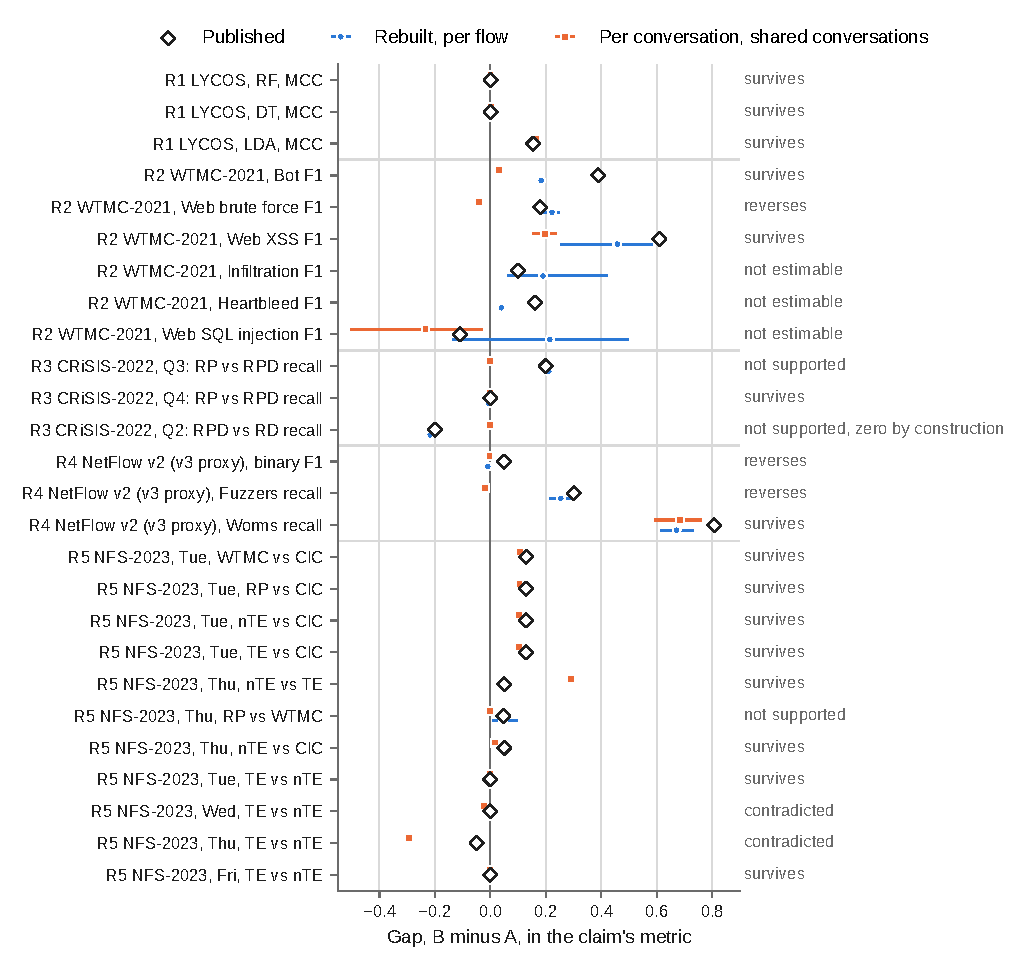
\includegraphics[width=\textwidth]{fig6_rq5_claims.pdf}
\caption{Every RQ5 contrast that could be rebuilt per flow: the gap as published, our per-flow rebuild, and the gap at the conversation unit on conversations present in both releases, the last two with \setnum{95} percent paired cluster bootstrap intervals; the verdict is at the right. A gap is one release minus another in the claim's own metric: the refined or corrected release (LYCOS, WTMC-2021, the later CRiSIS-2022 variant, NF-UNSW-NB15-v3) minus the release it was compared with for R1 to R4, and the first-named minus the second-named release for R5. R4 uses NF-UNSW-NB15-v3 in place of NF-UNSW-NB15-v2}\label{fig:rq5}
\end{figure*}

%% =====================================================================
\section{Discussion}\label{sec:discussion}
%% =====================================================================

%% Discussion (plan steps 10.6 and 7.4). Every number is a macro from tables/numbers.tex.
\paragraph{What a defined comparison of releases looks like.} One implication follows from RQ1 alone and does not depend on the detection results. Because flow-level recall weights each conversation by the number of records its exporter wrote (Eq.~\eqref{eq:flowrecall}), and because that number varies between releases by class (Table~\ref{tab:rq1-fpc}), a flow-level comparison between two releases of \cicids{} compares different estimands for every attack class except PortScan, whatever the detectors do. RQ5 shows that the difference is large enough to change published conclusions. A comparison of two releases is defined when it holds four things fixed: the conversations scored, the labels they carry, the split that sends them to training or test, and the unit at which they are counted. When all four are fixed, the gap that remains belongs to the exporter's features and segmentation as they reach the detector, which is what a claim that one release is better should be about. Fixing the labels includes a choice that is easy to miss: how a record without attack payload is labelled. Under the schedule label it is an attack, under a payload rule it is benign, and on \cicids{} that choice alone decides whether the RQ3 drop and the RQ4 residual appear (Sections~\ref{sec:rq3} and \ref{sec:rq4}). The conversation unit is not neutral, though. Under the ``any'' rule it turns an end-of-connection record that the schedule labels as attack into a false alarm on benign traffic (Section~\ref{sec:rq4}), and a byte-weighted rule removes that effect. A per-conversation score therefore needs its aggregation rule stated, as a per-flow score needs its split.

\paragraph{A reporting checklist.} Table~\ref{tab:checklist} turns these results into items that a producer of a flow release or an evaluator can apply without our code. Each item names the result that makes it necessary.

\begin{table*}[t]
\caption{Reporting checklist for flow releases and for evaluations that use them. Evidence: the result in this paper that makes the item necessary.}\label{tab:checklist}
\small
\begin{tabularx}{\textwidth}{@{}l>{\raggedright\arraybackslash}p{5.6cm}L@{}}
\toprule
Item & What to report & Evidence \\
\midrule
\multicolumn{3}{@{}l}{\emph{For producers of a flow release}} \\
P1 & The exporter, its version, every timeout and expiry setting (active, idle, FIN and RST expiry), and any filter applied after export. & Two releases of the same packets that differ in one expiry rule and the filter it triggers differ in records per conversation for most attack classes and in flow-level F1 (Section~\ref{sec:rq3}). \\
P2 & The five-tuple and the start and end timestamps of every record, at their native resolution. & Without them records cannot be grouped into conversations; the minute clock of the original \cicids{} release already forces a mapping step (Section~\ref{sec:key}). \\
P3 & The labelling rule (schedule, windows, what is dropped, how records without attack payload are labelled), and a flag wherever a record's label departs from it. & Scored against their own labels, the seven \cicids{} releases agree on the model ranking with $W$ of \RQfourOwnScoreWFlow{}, against \RQfourWFlow{} with one schedule truth (Section~\ref{sec:rq4}); under payload-aware labels the RQ3 drop disappears (Section~\ref{sec:rq3}). \\
\midrule
\multicolumn{3}{@{}l}{\emph{For evaluators}} \\
E1 & Split by conversation (endpoint pair, protocol and a gap $T$), never by record, and state whether larger units such as attack campaigns straddle the split. & The leakage of a random flow split differs by a factor of more than \RQoneLeakFactor{} between releases (Section~\ref{sec:rq1}); the conclusions do not change for $T$ from \NsweepCicStableMin{} to \setnum{120} seconds, and every \cicids{} attack episode straddles the split (Section~\ref{sec:rq4}). \\
E2 & Score per conversation as well as per record, on the conversations both releases contain, and state the aggregation rule. & Per conversation, \RQfiveReverse{} published contrasts reverse and \RQfiveContradicted{} claims of no difference fail (Section~\ref{sec:rq5}); the ``any'' rule creates the residual that a byte-weighted rule removes (Section~\ref{sec:rq4}). \\
E3 & Per-class F1 with the number of independent test units per class and seed: conversations, and episodes where the schedule defines them. & A flow count overstates the number of independent units by the records-per-conversation factor of the release (Table~\ref{tab:rq1-fpc}). \\
E4 & Flag, and leave out of a headline average, any class with fewer than \SetMinTest{} independent units on either side of the split or whose units all straddle it. & Heartbleed and Infiltration, below; \RQfiveNotEstimable{} published contrasts are not estimable for this reason (Section~\ref{sec:rq5}). \\
\bottomrule
\end{tabularx}
\end{table*}

Four classes show how the items work. \emph{Heartbleed} fails items E3 and E4. The whole class is one connection, written as \RQoneHeartbleedRecords{} records by every release except BCCC. Under the conversation-grouped split it is in training in all five seeds and never in test, so no conversation-level F1 exists for it; under a random flow split its records are divided between training and test, and an F1 reported for it measures how well a model recognises sibling records of a connection it was trained on. It should be reported as one unit that cannot be evaluated. \emph{Infiltration} fails items P3, E3 and E4. The schedule we use excludes it, and in the releases that label it all its conversations connect one pair of hosts, so it is at most one independent unit however the records are split; two releases do not contain it. \emph{UNSW-NB15 Backdoor} passes: it has \RQfourBackdoorTest{} test and \RQfourBackdoorTrain{} training conversations in every seed, and \RQfourBackdoorEpTest{} test episodes, of which \RQfourBackdoorEpStrad{} also have conversations in training. Reported with these counts, its F1 can be compared across releases. \emph{CICIDS2017 SSH-Patator} is a borderline case. It passes at the conversation level, with \RQfourSshTestConv{} test conversations per seed, but it is one campaign against one victim, and that campaign straddles every split, so its test conversations are independent of training only at the level of the conversation.

\paragraph{Near-perfect scores.} Near-perfect flow-level scores on \cicids{} are common \cite{maseer2021}. Our results do not show that such scores are inflated by leakage: in RQ3 the release that leaks most gains almost nothing from it, because the sibling record in training shares almost nothing with the record in test. They show something different. A flow-level score on one release refers to a population of records that another release of the same traffic does not have, with each conversation counted as many times as the exporter cut it. Two near-perfect scores on two releases are therefore not two measurements of the same detector quality, and their difference is not evidence that one release is better.

\paragraph{What we did not test.} Janati Idrissi et al.\ report a spread of up to \litnum{8.77} percent in macro-F1 between timeout settings \cite{janatiidrissi2025}. Their design changes the scored flows with every setting (Section~\ref{sec:related}), so the spread can come from the detectors or from the population, and we did not test how much of it the population change alone could produce; that needs a re-extraction of the captures over their grid, which is outside our scope of published releases. The UNSW-NB15 residual of RQ4 is not explained, and a feature ablation would be the next test. Own-label and payload-aware retraining were run on \cicids{} only.


%% =====================================================================
\section{Threats to validity}\label{sec:threats}
%% =====================================================================

%% Threats to validity (plan step 9.1). Written at the freeze, 28 October 2026, from
%% 00_Plan/Threats_and_Methods_Notes.md (notes 1 to 26) and the Phase 5 to 8 notes. Every number is
%% a macro from 05_Paper/tables/numbers.tex. Each paragraph names a choice, the risk it carries and
%% what we did about it.

Each methods choice below is stated with the risk it carries and what we did to bound it. We group them by the validity type they threaten.

\paragraph{Construct validity: what the ground truth means.} The labels come from an attack schedule (Section~\ref{sec:gt}). A benign conversation is one outside every attack window, not one that was checked to be benign, and the schedule's drop rules remove Thursday afternoon, so \cicids{} has no infiltration class here. The window ends we reuse differ from those of the NFS-2023 labeller (SSH-Patator ends \NsshWindowEndMinutes{} minutes earlier in our schedule), which moves a few conversations at window edges from attack to benign. A schedule label also makes every record of an attack conversation an attack record, including records an exporter writes after the attack payload has ended (Section~\ref{sec:gt}). We chose the schedule because it is the only label that is the same in every arm by construction, so the comparison isolates the exporter; the cost is that a detector is asked to flag a record that carries no attack payload. That cost is measurable, and it is not small. Under payload-aware labels the RQ3 drop disappears, the RQ4 residual on \cicids{} disappears, and H2 on \cicids{} no longer holds by the strict-majority rule (Sections~\ref{sec:rq2} to \ref{sec:rq4}). The exporter results on \cicids{} are therefore results about exporters under one label policy, the one that makes the arms comparable, and the label policy for records without payload is a second choice that an evaluator has to state. Each arm's own labels are kept as a further setting (Section~\ref{sec:rq4}); with them the releases agree far less on which model is best.

\paragraph{Construct validity: attempted attacks.} Conversations that the schedule calls an attack but that carry no payload stay under their schedule class in the primary analysis, because the attacker sent the traffic and an operator would want the attempt detected. CRiSIS-2022 and both NFS-2023 releases label most of these benign by policy (Section~\ref{sec:gt}). Folding them into benign is a frozen sensitivity setting. In RQ4 it changes the H4 verdict only when the folded labels are used for scoring a model trained without them; retrained on the folded labels, H4 is undecided as in the primary setting and H2 is unchanged, while \RQfourFoldRetrainedClasses{} of \RQfourClassesOf{} per-class verdicts at the conversation unit change. In RQ5 one reversal, WTMC-2021 on Web brute force, depends on this rule and is reported as fragile.

\paragraph{Construct validity: the unit.} A conversation is defined by the endpoint pair, the protocol and a silence of more than $T = \SetT$ seconds (Section~\ref{sec:key}). On \cicids{} every scored class has the same conversation count from \NsweepCicStableMin{} to \NsweepCicStableMax{} seconds; larger values merge distinct DDoS and DoS Hulk conversations because their tools reuse endpoint keys. On UNSW-NB15, Generic splits into \NsweepGenericFivePct{} percent more conversations at \NsweepCicStableMin{} seconds than at \SetT{}, so a shorter $T$ would change that class. The RQ4 conclusions are rerun over $T$ in Section~\ref{sec:rq4}. A conversation is also not independent of its neighbours: one attack campaign holds many conversations, and a campaign can straddle the split, as SSH-Patator does in every seed. Our grouped split removes leakage between records of one conversation, not between conversations of one campaign. The ``any'' rule turns a conversation into a false alarm when a single record is flagged, which penalises releases that write short tail records; the majority and byte-weighted rules are reported beside it.

\paragraph{Internal validity: the instrument.} The original \cicids{} release has a minute clock and does not take part in defining conversations; its records are mapped afterwards, and up to \NnondefAmbigMax{} of them per day have more than one candidate conversation. That arm also comes from the GeneratedLabelledFlows files, because the better known machine learning CSV files carry no five-tuple and no timestamp. The two have the same row count (\NcicRows{}), but we did not compare their feature values row by row, so a result on our CIC original arm transfers to the machine learning files only if their features agree. Clocks were reconciled by us against the published schedule (Section~\ref{sec:clocks}). A wrong offset would misalign whole windows; each offset was chosen so that the attack windows line up with the schedule, and the window edges that still differ after it are kept in the release clock table of the replication files rather than corrected. The record alignment was checked by hand on \NhandCases{} conversations chosen to cover every cardinality class; the check found \docnum{four} faults, all fixed and held by unit tests, but \NhandCases{} cases is a small sample, and the pairing rule could still be wrong on patterns the sample did not contain.

\paragraph{Internal validity: the releases.} Two choices about UNSW-NB15 change its numbers. Exact duplicate lines are dropped for RQ1 and RQ2 and kept for RQ5, where published results used them; near repeats are collapsed in a sensitivity arm only. The near repeat definition is ours (same five-tuple, start, end and byte count after exact duplicates are gone), and a different one would remove a different set of records; neither sensitivity arm changes the H2 verdict. The H2 verdict on UNSW-NB15 does depend on CIC-UNSW-NB15, the release whose records score lowest: without it, H2 does not hold on that benchmark (Section~\ref{sec:rq2}). The NFS-2023 pair differs downstream of the exporter as well, through a filter that the expiry rule triggers and through its own labeller, so RQ3 measures one generator setting together with the filter it triggers. Of the split behaviours traced in Section~\ref{sec:rq1}, the third FTP-Patator record in CIC original is only partly explained, and which benign records NFS-2023-TE writes that models take for DoS Hulk is not explained.

\paragraph{Internal validity: the detection experiment.} The grid runs on a subsample that keeps \SetBenignFraction{} of benign conversations and at most \SetAttackCap{} conversations per attack class. This raises attack prevalence, so precision and F1 are higher than they would be on the full data. The same conversations are kept in every arm, so the subsample does not favour one exporter, but absolute F1 values are not full-data values. Reweighting each test conversation to full-data prevalence leaves recall unchanged and lowers precision, on average over arms and models, by at most \RevHtPrecMeanMaxCic{} for a \cicids{} attack class and \RevHtPrecMeanMaxUnsw{} for a UNSW-NB15 one; H2 still holds on both benchmarks under these weights (Table~\ref{tab:rev-robust}). We also trained the random forest on all records of every arm, on seed \setnum{0} of the grouped split, and scored it on all test records. For \RevFullWithinFive{} percent of the \RevFullPairs{} pairs of arm and attack class with at least \setnum{20} test records, flow F1 changed by at most \setnum{0.05} (median change \RevFullFoneMedian{}), and precision fell by at most \RevFullPrecMaxFall{}. The exception is the UNSW-NB15 Fuzzers class, whose recall falls by \RevFullFuzzRecallMin{} to \RevFullFuzzRecallMax{} across arms when the model is trained with all benign traffic, so that its F1 falls by up to \RevFullFoneMaxAbs{}. Absolute UNSW-NB15 Fuzzers scores in this paper are therefore subsample scores; this check has one model and one seed and does not test the H2 verdict on the full data. The conversation-level contrasts of RQ5 are on the subsample, and we did not reweight them; the RQ5 table states which metrics depend on prevalence. Hyperparameters were tuned once per arm and model, on seed \setnum{0} of the grouped split, from a grid of \SetGridSize{} settings; a model that suits one release better under a wider search would show up here as part of the exporter or interaction share. LightGBM was given an L2 penalty after its training diverged on the first arm tuned, before any grid cell was run. Identifiers are removed from the features. Time-to-live fields in UNSW-NB15 could act as a shortcut; removing them from every UNSW-NB15 arm leaves the H2 verdict there unchanged (Section~\ref{sec:rq2}). The software is deterministic: \RQtwoReproCells{} cells rerun from scratch gave identical predictions, and the whole result set is regenerated from the raw releases in one run.

\paragraph{Internal validity: rebuilt published comparisons.} RQ5 rebuilds each claim as the authors framed it, but not always with their setup: we ran a subset of their algorithms where they tested several, used our own hyperparameters and feature lists where we did not take theirs, seeded models they left unseeded, and used NF-UNSW-NB15-v3 for the conversation-level check of a claim made on NF-UNSW-NB15-v2, which has no timestamps. Where our per-flow rebuild did not reproduce the published value, the verdict is about our rebuild of the comparison, not about the authors' run.

\paragraph{External validity.} Two benchmarks, both recorded in laboratory testbeds, and only published releases; no packet capture was re-extracted by us. Releases we could not obtain are not covered: the HERA versions of \cicids{} and every release of CSE-CIC-IDS2018. Exporters not represented among the releases, such as Zeek and Argus on \cicids, enter only through the literature. The models of the primary grid are three tabular learners, two of them tree ensembles, and the extension adds two more of a different kind; sequence models that read several records of a conversation at once may react differently to how an exporter cuts it.

\paragraph{Statistical conclusion validity.} The confirmatory family is H2 and H4, each judged once by a rule fixed before training; every other comparison, including the per-class verdicts that make up H2, is descriptive, and the per-class intervals are not adjusted for multiplicity. Bootstrap intervals resample conversations, so they treat conversations of one campaign as independent and are too narrow if anything; the alpha intervals share that limit. The variance shares of RQ2 are shares of the sum of squares, and the arm factor has six degrees of freedom on \cicids{} and two on UNSW-NB15 against two for the model. Omega squared, computed afterwards as a check, lies within \NomegaMaxGap{} of the share for every eligible small class and changes the direction of \NomegaChanged{} class that the interval rule decides. Shares per degree of freedom, which do correct for a factor with more levels being able to spread further, keep H2 on both benchmarks, with fewer \cicids{} classes to the exporter (Table~\ref{tab:rev-robust}). The robustness analyses were added after the primary results and are not adjusted for multiplicity; we read them as checks on the verdicts, not as further tests. With three arms on UNSW-NB15 and three models, Kendall's $W$ can take only a few values (\RQfourWFlowUnsw{} at the flow unit and \RQfourWConvUnsw{} at the conversation unit on the common population), so H4 on that benchmark is weak evidence either way. The seed share of \RQtwoSeedUnswBenign{} for the UNSW-NB15 benign class is the largest on that benchmark but small next to the exporter and model shares. The RQ3 permutation test has \RQthreeClasses{} classes and little power, which is why its result is reported as supported in direction only.


%% =====================================================================
\section{Conclusion}\label{sec:conclusion}
%% =====================================================================

We asked whether a score difference between two exported releases of a benchmark says anything about the releases, and found that, as usually computed, it compares different populations. Seven releases of \cicids{} and three of UNSW-NB15 agree on which conversations occurred and disagree, by class and by termination rule, on how many records each one becomes. That disagreement changes the leakage of the field's default split and the weight of each conversation in a flow-level score, and on both benchmarks the exporter explains more of the variation in per-class F1 than the model for most small classes, on UNSW-NB15 only with CIC-UNSW-NB15 among the releases and with the three primary models. Part of that share on \cicids{} comes through the label given to records without payload, which a payload-aware rule removes. Scoring each conversation once, on a split by conversation, removes most of the exporter's share and makes more between-release comparisons equivalent within a stated margin, but not all of them; it does not make model rankings more consistent, and with five models they agree less on \cicids{}; it also brings its own artefact, which the aggregation rule decides. When published comparisons of releases are redone on the same conversations with one truth, \RQfiveSurvive{} of the \RevFiveDecided{} contrasts that can be decided survive, often much smaller, and the rest reverse, are contradicted or lose their support per conversation. A release should be judged by a comparison that holds the traffic, the labels, the split and the unit fixed, and the checklist of Table~\ref{tab:checklist} lists what producers and evaluators need to report for such a comparison to be possible. The next steps are a feature ablation for the UNSW-NB15 residual and the same instrument applied to re-extractions of the packet captures, where the exporter settings can be varied one at a time.

\backmatter

\bmhead{Acknowledgements}
We thank Md.\ Badiuzzaman Biplob, Lecturer, Department of Computer Science and Engineering, International Islamic University Chittagong, for supervising this work. We also thank the authors of every release used here for making their data public.

\section*{Statements and declarations}\label{sec:declarations}

\begin{itemize}
\item \textbf{Funding.} The authors received no funding for this work.
\item \textbf{Competing interests.} The authors declare no competing interests.
\item \textbf{Ethics approval and consent.} Not applicable; the study uses only public datasets of synthetic and testbed traffic.
\item \textbf{Data availability.} All releases analysed are public from their authors: \cicids{} \cite{sharafaldin2018}, WTMC-2021 \cite{engelen2021}, CRiSIS-2022 \cite{lanvin2023}, LYCOS-IDS2017 \cite{rosay2021}, NFS-2023 \cite{pekar2024}, BCCC-CIC-IDS2017 \cite{shafi2024}, UNSW-NB15 \cite{moustafa2015}, NF-UNSW-NB15-v3 \cite{luay2026} and CIC-UNSW-NB15 \cite{mohammadian2024}. The record-level instrument tables are derived from these releases and are not redistributed, in line with their licences; the scripts rebuild them from the public files, and the aggregate result files and manifests are in the code repository.
\item \textbf{Code availability.} \url{https://github.com/26sudipta/same-packets-different-scores}, public, with the version used for this paper archived on Zenodo (\tocheck{DOI of the Zenodo deposit}).
\item \textbf{Use of AI tools.} An AI assistant (Claude, Anthropic) was used to search and verify literature records, to write and test analysis code under the authors' direction, and to draft text that the authors revised. Every reference was checked against its publisher or arXiv record, and every number was regenerated by the scripts of Section~\ref{sec:method}. The authors take full responsibility for the content.
\item \textbf{Author contributions.} Sudipta Das: conceptualization, methodology, software, formal analysis, writing (original draft). Nayan Nath: validation, investigation, writing (review and editing). Both authors read and approved the final manuscript.
\end{itemize}

\begin{appendices}
%% Appendices (plan step 10.8). Numbers are macros or protocol constants (\setnum).
\renewcommand{\theHtable}{app.\thetable}% link targets of the appendix tables must differ from Tables 1 to 4
\section{The instrument step by step}\label{app:instrument}

The steps below are what \texttt{instrument.py} and \texttt{build\_instrument.py} do for one benchmark and one capture day. Each step names the section of the paper that motivates it.

\begin{enumerate}
\item \emph{Load and clock.} Read every arm's records for the day, convert start times to UTC with the arm's offset (Section~\ref{sec:clocks}), and give each record the interval from its start to its start plus its duration plus the resolution of its arm's clock. UNSW-NB15 start times, which are rounded, are shifted by half the resolution first.
\item \emph{Key.} Give each record the key (lower endpoint, higher endpoint, protocol), with an endpoint written as address and port, ports set to zero for protocols other than TCP and UDP, and every protocol other than ICMP, TCP and UDP put in one class (Section~\ref{sec:key}).
\item \emph{Conversations.} Pool the records of the defining arms, which are all arms except CIC original. Sort them by key, start and end. Walking through each key in that order, a record opens a new conversation when its start is more than $T$ after the latest end seen so far for the key.
\item \emph{Mapping.} For each CIC original record, take the latest conversation of the same key that starts before the record's latest possible start, and up to \setnum{3} conversations before that one. A candidate is reachable when the record starts within $T$ of its end. The record joins the reachable candidate whose span is closest to the record's duration, ties going to the later one. Records with no reachable candidate form conversations of their own by the rule of the previous step and are counted as unmapped.
\item \emph{Initiator.} The initiator is the source endpoint of the earliest record of the conversation; a record whose source is the other endpoint is marked as reversed.
\item \emph{Ground truth.} Label each conversation from the attack schedule (Section~\ref{sec:gt}): \cicids{} conversations by attacker, victim, port, protocol and window, with the endpoints in either order and the conversation start inside the window, and the drop rules giving the label ``excluded''; UNSW-NB15 conversations from the ground truth file on the same key by overlap of intervals, the most frequent category winning. Every record takes the label of its conversation.
\item \emph{Pairing.} For each pair of arms and each conversation both have, form every pair of their records whose intervals overlap. Rank the pairs by the gap between their start windows, then by the difference in duration, then same direction before reversed, then larger overlap, then smaller raw start difference, and assign them greedily one to one. When a conversation has more than \setnum{250{,}000} candidate pairs, pair its records in time order instead. Records left without a partner stay unpaired. Record the cardinality class of the conversation for the pair of arms.
\item \emph{Episodes.} Group the attack conversations of one class between one pair of hosts: on \cicids{} within one schedule window, on UNSW-NB15 by the rule of the conversation step applied with a gap of \setnum{300} seconds.
\item \emph{Splits.} For each seed, hash an identifier of each conversation (benchmark, day, key and start) with a seeded SipHash, and within each class and day send the lowest \SetTestPct{} percent of hashes to the test set. The random flow split applies the same rule to records, per arm and class.
\item \emph{Freeze.} Write the conversation table, the record to conversation map and the pairs with a manifest of input hashes, settings and the code version.
\end{enumerate}

The \NhandCases{} hand-checked conversations of Section~\ref{sec:method} are frozen as unit test fixtures of these steps.

\section{Models, hyperparameters and seeds}\label{app:models}

All models are from scikit-learn and LightGBM at the versions pinned with the code. The random forest has \setnum{100} trees. LightGBM has \setnum{200} boosting rounds, an L2 penalty of \setnum{1} on leaf values, and deterministic, row-wise training. The multilayer perceptron applies a signed log transform and standard scaling, and trains with early stopping for at most \setnum{50} epochs in batches of \setnum{512}. Each model's grid has \SetGridSize{} settings: for the random forest, maximum depth unlimited or \setnum{20} crossed with a minimum of \setnum{1} or \setnum{3} samples per leaf; for LightGBM, \setnum{31} or \setnum{127} leaves crossed with a learning rate of \setnum{0.1} or \setnum{0.05}; for the multilayer perceptron, one hidden layer of \setnum{64} units or two of \setnum{128} and \setnum{64}, crossed with an L2 penalty of \setnum{0.0001} or \setnum{0.001}. Tuning uses seed \setnum{0} of the grouped split, with a validation set of \SetValPct{} percent of the training conversations drawn by the same hash rule with its own seed. The seed of a cell, one of \SetSeeds{}, selects both the split and the model's random state. Table~\ref{tab:hyper} gives the setting chosen for each arm.

% Generated by 03_Code/make_numbers.py from 04_Results/phase5/tuning.csv. Do not edit by hand.
\begin{table*}[t]
\caption{Hyperparameter setting chosen for each arm and model from the grid of four settings per
model, by validation macro-F1 on seed 0 of the grouped split. Random forest: maximum depth and
minimum samples per leaf. LightGBM: number of leaves and learning rate. Multilayer perceptron:
hidden layer sizes and L2 penalty. UNSW-NB15 original is the release with duplicate records dropped; the
sensitivity arms of UNSW-NB15 are not listed.}\label{tab:hyper}
\small
\setlength{\tabcolsep}{4pt}
\begin{tabular}{@{}lllll@{}}
\toprule
 & & Random forest & LightGBM & Multilayer perceptron \\
Benchmark & Arm & depth / leaf & leaves / rate & layers / L2 \\
\midrule
CICIDS2017 & CIC original & none / 1 & 31 / 0.05 & (128, 64) / 0.001 \\
 & WTMC-2021 & none / 1 & 127 / 0.1 & (64) / 0.001 \\
 & CRiSIS-2022 & none / 3 & 127 / 0.05 & (128, 64) / 0.001 \\
 & LYCOS & none / 1 & 31 / 0.05 & (128, 64) / 0.001 \\
 & NFS-2023-nTE & none / 1 & 127 / 0.05 & (128, 64) / 0.0001 \\
 & NFS-2023-TE & none / 3 & 31 / 0.05 & (128, 64) / 0.001 \\
 & BCCC & none / 1 & 31 / 0.1 & (128, 64) / 0.001 \\
\midrule
UNSW-NB15 & UNSW-NB15 original & none / 1 & 31 / 0.1 & (128, 64) / 0.001 \\
 & NF-UNSW-NB15-v3 & none / 1 & 127 / 0.05 & (128, 64) / 0.0001 \\
 & CIC-UNSW-NB15 & 20 / 1 & 31 / 0.1 & (128, 64) / 0.0001 \\
\bottomrule
\end{tabular}
\end{table*}


\section{Per-class F1}\label{app:f1}

Tables~\ref{tab:f1-cic} and \ref{tab:f1-unsw} give per-class F1 at both units on the common population, the setting of RQ4.

% Generated by 03_Code/make_numbers.py from 04_Results/phase5/results.csv. Do not edit by hand.
\begin{table}[t]
\caption{Per-class F1 on CICIDS2017 at the flow unit and at the conversation unit, grouped
split, common population, mean over three models and five seeds. Classes with no test conversation in
any seed do not appear.}\label{tab:f1-cic}
\small
\setlength{\tabcolsep}{4pt}
\begin{tabular}{@{}lrrrrrrr@{}}
\toprule
Class & \rotatebox{90}{CIC original} & \rotatebox{90}{WTMC-2021} & \rotatebox{90}{CRiSIS-2022} & \rotatebox{90}{LYCOS} & \rotatebox{90}{NFS-2023-nTE} & \rotatebox{90}{NFS-2023-TE} & \rotatebox{90}{BCCC} \\
\midrule
\multicolumn{8}{@{}l}{\emph{Flow unit}} \\
Benign & 0.997 & 0.999 & 0.999 & 0.999 & 0.999 & 0.979 & 0.987 \\
Bot & 0.932 & 0.997 & 0.998 & 0.998 & 0.998 & 0.666 & 0.845 \\
DDoS & 0.999 & 1.000 & 1.000 & 1.000 & 1.000 & 1.000 & 1.000 \\
DoS GoldenEye & 0.988 & 0.987 & 0.987 & 0.986 & 0.983 & 0.772 & 0.986 \\
DoS Hulk & 0.994 & 0.999 & 0.999 & 1.000 & 1.000 & 0.934 & 0.938 \\
DoS Slowhttptest & 0.986 & 0.987 & 0.987 & 0.985 & 0.977 & 0.976 & 0.954 \\
DoS Slowloris & 0.994 & 0.997 & 0.997 & 0.995 & 0.992 & 0.990 & 0.970 \\
FTP-Patator & 0.961 & 1.000 & 1.000 & 1.000 & 1.000 & 0.999 & 0.915 \\
PortScan & 1.000 & 1.000 & 1.000 & 1.000 & 1.000 & 0.999 & 0.998 \\
SSH-Patator & 0.993 & 0.997 & 0.997 & 0.997 & 0.996 & 0.667 & 0.959 \\
Web SQL injection & 0.351 & 0.483 & 0.441 & 0.413 & 0.424 & 0.271 & 0.466 \\
Web XSS & 0.251 & 0.294 & 0.287 & 0.276 & 0.275 & 0.134 & 0.479 \\
Web brute force & 0.769 & 0.766 & 0.771 & 0.764 & 0.759 & 0.539 & 0.626 \\
\midrule
\multicolumn{8}{@{}l}{\emph{Conversation unit (rule ``any'')}} \\
Benign & 0.997 & 0.999 & 0.999 & 0.999 & 0.999 & 0.988 & 0.991 \\
Bot & 0.944 & 0.997 & 0.998 & 0.998 & 0.998 & 0.999 & 0.929 \\
DDoS & 1.000 & 1.000 & 1.000 & 1.000 & 1.000 & 1.000 & 1.000 \\
DoS GoldenEye & 0.985 & 0.987 & 0.986 & 0.986 & 0.985 & 0.982 & 0.986 \\
DoS Hulk & 0.995 & 1.000 & 1.000 & 1.000 & 1.000 & 0.872 & 0.945 \\
DoS Slowhttptest & 0.985 & 0.985 & 0.986 & 0.984 & 0.985 & 0.983 & 0.980 \\
DoS Slowloris & 0.995 & 0.996 & 0.996 & 0.995 & 0.995 & 0.994 & 0.991 \\
FTP-Patator & 0.915 & 1.000 & 1.000 & 1.000 & 1.000 & 0.999 & 0.972 \\
PortScan & 1.000 & 1.000 & 1.000 & 1.000 & 1.000 & 1.000 & 0.999 \\
SSH-Patator & 0.994 & 0.997 & 0.997 & 0.997 & 0.997 & 0.995 & 0.933 \\
Web SQL injection & 0.513 & 0.483 & 0.441 & 0.413 & 0.424 & 0.460 & 0.503 \\
Web XSS & 0.120 & 0.294 & 0.287 & 0.276 & 0.275 & 0.228 & 0.358 \\
Web brute force & 0.798 & 0.766 & 0.771 & 0.764 & 0.759 & 0.777 & 0.648 \\
\bottomrule
\end{tabular}
\end{table}

% Generated by 03_Code/make_numbers.py from 04_Results/phase5/results.csv. Do not edit by hand.
\begin{table}[t]
\caption{Per-class F1 on UNSW-NB15 at the flow unit and at the conversation unit, grouped
split, common population, mean over three models and five seeds. Classes with no test conversation in
any seed do not appear.}\label{tab:f1-unsw}
\small
\setlength{\tabcolsep}{4pt}
\begin{tabular}{@{}l>{\centering\arraybackslash}p{2.8cm}>{\centering\arraybackslash}p{2.8cm}>{\centering\arraybackslash}p{2.8cm}@{}}
\toprule
Class & UNSW-NB15 original, duplicates dropped & NF-UNSW-NB15-v3 & CIC-UNSW-NB15 \\
\midrule
\multicolumn{4}{@{}l}{\emph{Flow unit}} \\
Benign & 0.993 & 0.993 & 0.992 \\
Analysis & 0.386 & 0.199 & 0.161 \\
Backdoor & 0.650 & 0.744 & 0.443 \\
DoS & 0.434 & 0.563 & 0.255 \\
Exploits & 0.846 & 0.895 & 0.690 \\
Fuzzers & 0.852 & 0.866 & 0.658 \\
Generic & 0.962 & 0.969 & 0.563 \\
Reconnaissance & 0.919 & 0.927 & 0.716 \\
Shellcode & 0.657 & 0.833 & 0.282 \\
Worms & 0.424 & 0.691 & 0.321 \\
\midrule
\multicolumn{4}{@{}l}{\emph{Conversation unit (rule ``any'')}} \\
Benign & 0.993 & 0.992 & 0.992 \\
Analysis & 0.364 & 0.202 & 0.243 \\
Backdoor & 0.654 & 0.763 & 0.681 \\
DoS & 0.420 & 0.535 & 0.399 \\
Exploits & 0.848 & 0.870 & 0.820 \\
Fuzzers & 0.851 & 0.864 & 0.797 \\
Generic & 0.769 & 0.869 & 0.751 \\
Reconnaissance & 0.920 & 0.927 & 0.903 \\
Shellcode & 0.658 & 0.833 & 0.366 \\
Worms & 0.426 & 0.692 & 0.484 \\
\bottomrule
\end{tabular}
\end{table}


\section{Conversations at every gap}\label{app:tsweep}

Table~\ref{tab:tsweep} gives the number of conversations per class at every value of $T$ in the sweep of Section~\ref{sec:key}.

% Generated by 03_Code/make_numbers.py from 04_Results/phase3/all_gap_sweep.csv. Do not edit by hand.
\begin{table*}[t]
\caption{Conversations per class at every value of the gap $T$ in the sweep, summed over all
capture days (five on CICIDS2017, two on UNSW-NB15). The primary analysis uses $T = \SetT$ s. Conversations excluded by the schedule's drop
rules are not counted.}\label{tab:tsweep}
\small
\setlength{\tabcolsep}{4pt}
\begin{tabular*}{\textwidth}{@{\extracolsep{\fill}}lrrrrrr@{}}
\toprule
 & \multicolumn{6}{c}{Gap $T$ (seconds)} \\
\cmidrule(l){2-7}
Class & 5 & 15 & 30 & 60 & 120 & 300 \\
\midrule
\multicolumn{7}{@{}l}{\emph{CICIDS2017}} \\
Benign & 1{,}283{,}325 & 1{,}282{,}873 & 1{,}282{,}777 & 1{,}282{,}768 & 1{,}282{,}675 & 1{,}280{,}604 \\
Bot & 736 & 736 & 736 & 736 & 736 & 736 \\
DDoS & 93{,}178 & 93{,}178 & 93{,}178 & 92{,}980 & 63{,}540 & 63{,}540 \\
DoS GoldenEye & 6{,}770 & 6{,}770 & 6{,}770 & 6{,}770 & 6{,}770 & 6{,}770 \\
DoS Hulk & 158{,}517 & 158{,}517 & 158{,}517 & 158{,}517 & 14{,}375 & 14{,}215 \\
DoS Slowhttptest & 4{,}369 & 4{,}369 & 4{,}369 & 4{,}369 & 4{,}369 & 4{,}219 \\
DoS Slowloris & 3{,}899 & 3{,}899 & 3{,}899 & 3{,}899 & 3{,}899 & 3{,}899 \\
FTP-Patator & 3{,}992 & 3{,}992 & 3{,}992 & 3{,}992 & 3{,}992 & 3{,}992 \\
Heartbleed & 1 & 1 & 1 & 1 & 1 & 1 \\
PortScan & 160{,}057 & 160{,}057 & 160{,}057 & 160{,}057 & 159{,}990 & 159{,}840 \\
SSH-Patator & 2{,}959 & 2{,}959 & 2{,}959 & 2{,}959 & 2{,}959 & 2{,}959 \\
Web SQL injection & 12 & 12 & 12 & 12 & 12 & 12 \\
Web XSS & 662 & 662 & 662 & 662 & 662 & 662 \\
Web brute force & 1{,}361 & 1{,}361 & 1{,}361 & 1{,}361 & 1{,}361 & 1{,}361 \\
\midrule
\multicolumn{7}{@{}l}{\emph{UNSW-NB15}} \\
Benign & 1{,}960{,}429 & 1{,}959{,}319 & 1{,}958{,}314 & 1{,}954{,}710 & 1{,}954{,}507 & 1{,}953{,}646 \\
Analysis & 427 & 427 & 427 & 427 & 425 & 405 \\
Backdoor & 355 & 355 & 355 & 355 & 355 & 355 \\
DoS & 3{,}636 & 3{,}636 & 3{,}636 & 3{,}636 & 3{,}636 & 3{,}636 \\
Exploits & 25{,}565 & 25{,}562 & 25{,}541 & 25{,}541 & 25{,}538 & 25{,}528 \\
Fuzzers & 19{,}374 & 19{,}373 & 19{,}372 & 19{,}367 & 19{,}354 & 19{,}185 \\
Generic & 3{,}844 & 3{,}740 & 3{,}736 & 3{,}735 & 3{,}733 & 3{,}732 \\
Reconnaissance & 11{,}630 & 11{,}630 & 11{,}630 & 11{,}630 & 11{,}630 & 11{,}629 \\
Shellcode & 1{,}511 & 1{,}511 & 1{,}511 & 1{,}511 & 1{,}511 & 1{,}511 \\
Worms & 158 & 158 & 158 & 158 & 158 & 158 \\
\bottomrule
\end{tabular*}
\end{table*}


\end{appendices}

\bibliography{refs}

\end{document}
